\section{Задача стабилизации с идеальным дифференцирующим звеном}

Рассмотрим объект управления 2-го порядка, заданный дифференциальным уравнением
\begin{equation*}
    a_2\ddot y+a_1\dot y + a_0 y=u. 
\end{equation*}
Возьмем коэффициенты $a_2=1,\ a_1=-3,\ a_0=2$, тогда система будем иметь два
неустойчивых полюса: $1,\ 2$. Зададимся начальными условиями $y(0)=1$ и $y'(0)=-2$.
Было выполнено моделирование (см. схему на рисунке \ref{fig:task_1_xls}) свободного движения системы, которое можно увидеть на
рисунке \ref{fig:task_1_out}.
\begin{figure}[H]
    \centering
    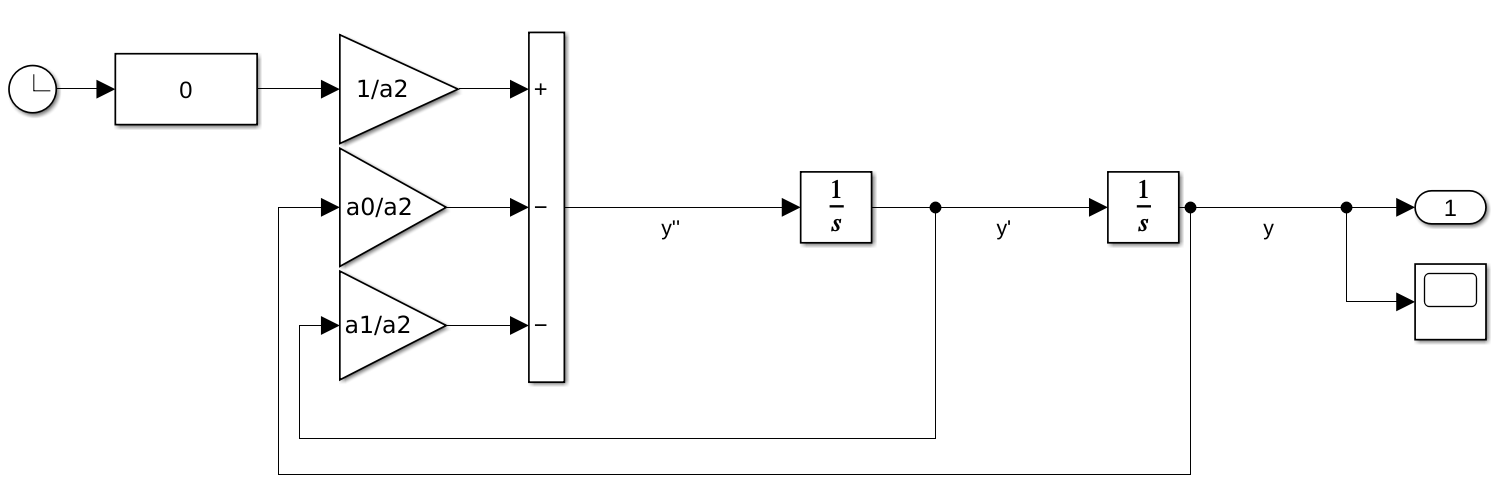
\includegraphics[width=1\textwidth]{figs/task_1_slx.png}
    \caption{Структурная схема для моделирования свободного движения}
    \label{fig:task_1_xls}
\end{figure}
\begin{figure}[H]
    \centering
    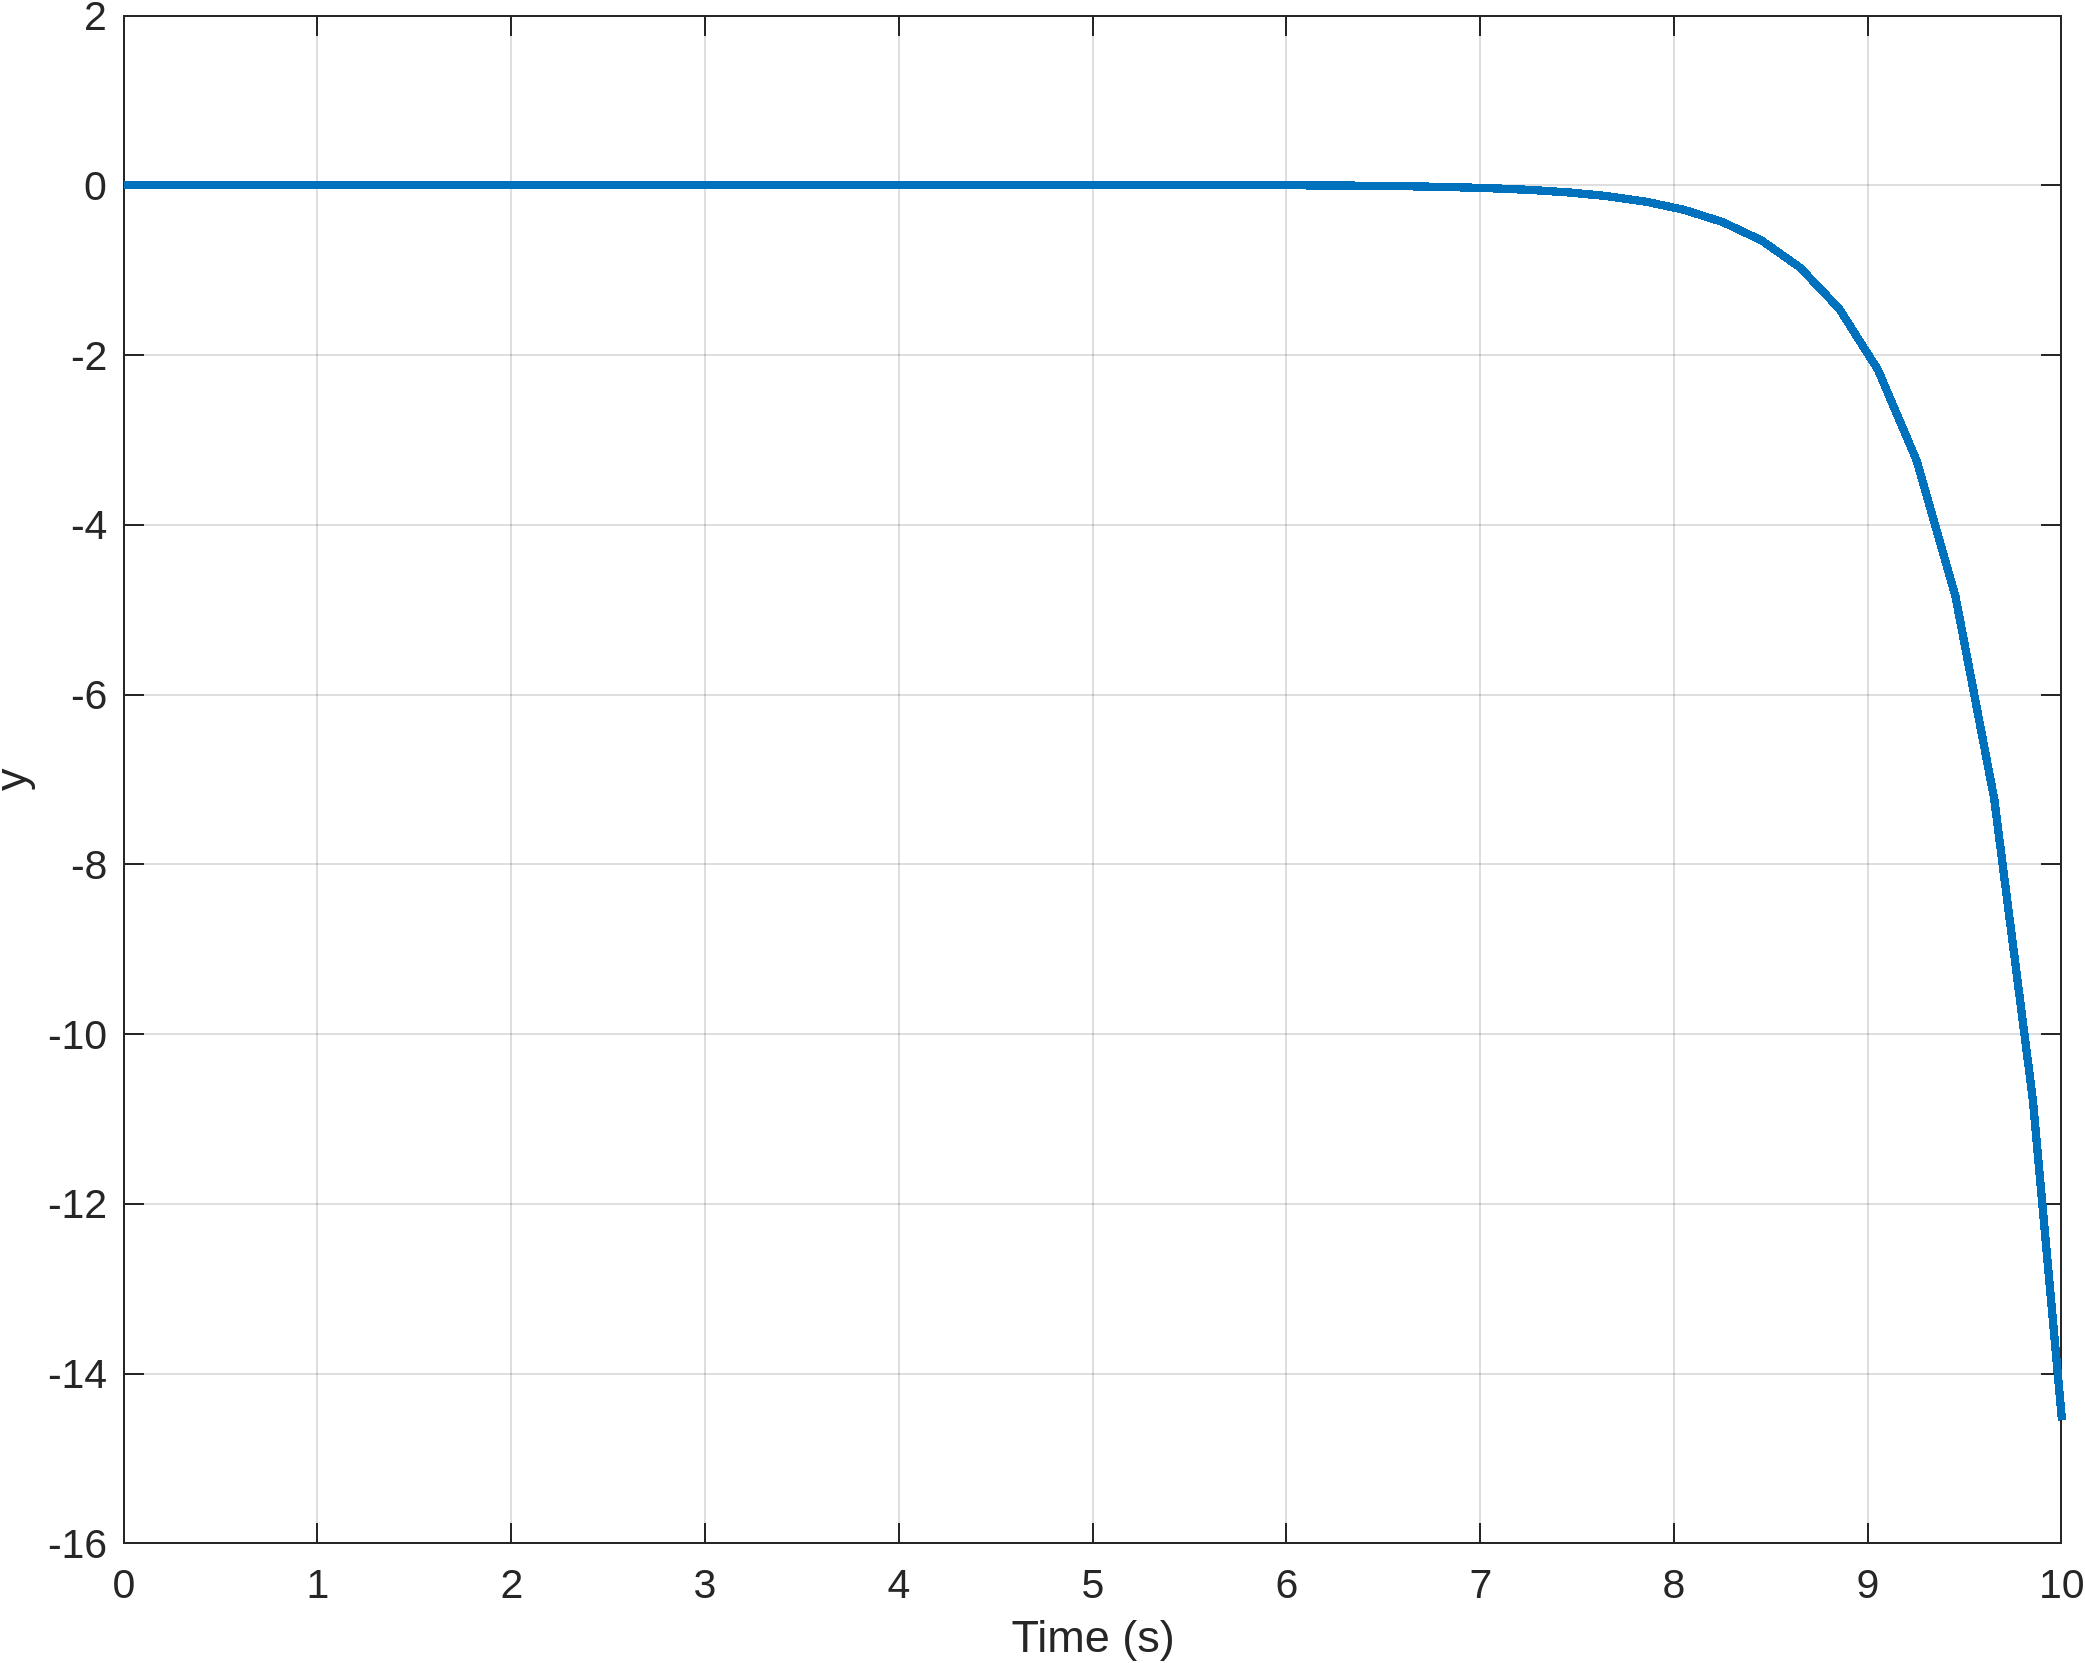
\includegraphics[width=0.8\textwidth]{figs/task_1_out.png}
    \caption{Свободное движение}
    \label{fig:task_1_out}
\end{figure}

Рассмотрим регулятор вида
\begin{equation*}
    u=k_0y+k_1\dot y
\end{equation*}
и построить структурную схему (см. рисунок \ref{fig:task_1_xls}). Можно аналитически
найти корни для асимптотической устойчивости, для этого рассмотрим характеристическое уравнение:
\[
    \lambda^2 + (-3 - k_1)\lambda + (2 - k_0) = 0.
\]
Для того чтобы вещественная часть корней была отрицательной, рассмотрим теорему
Виета:
\[
    \lambda_1 + \lambda_2 = 3 +k_1,
\]
\[
    \lambda_1 \cdot \lambda_2 = 2 -k_0,
\]
тогда получаем условия
\begin{equation*}
    \begin{array}{c}
        k_1<-3,\\
        k_0<2.
    \end{array}
\end{equation*}
Возьмем $k_0=1,\ k_1=-4$, чтобы система стала асимптотически устойчивой.
Результат моделирования для начальных условий из предыдущего моделирования можно увидеть
на рисунке \ref{fig:task_1_out_1}.

Как можно видеть, система стала устойчивой и сходится к нулю - единственной точке равновесия
линейных систем, в отличии от системы задания 1.
\begin{figure}[H]
    \centering
    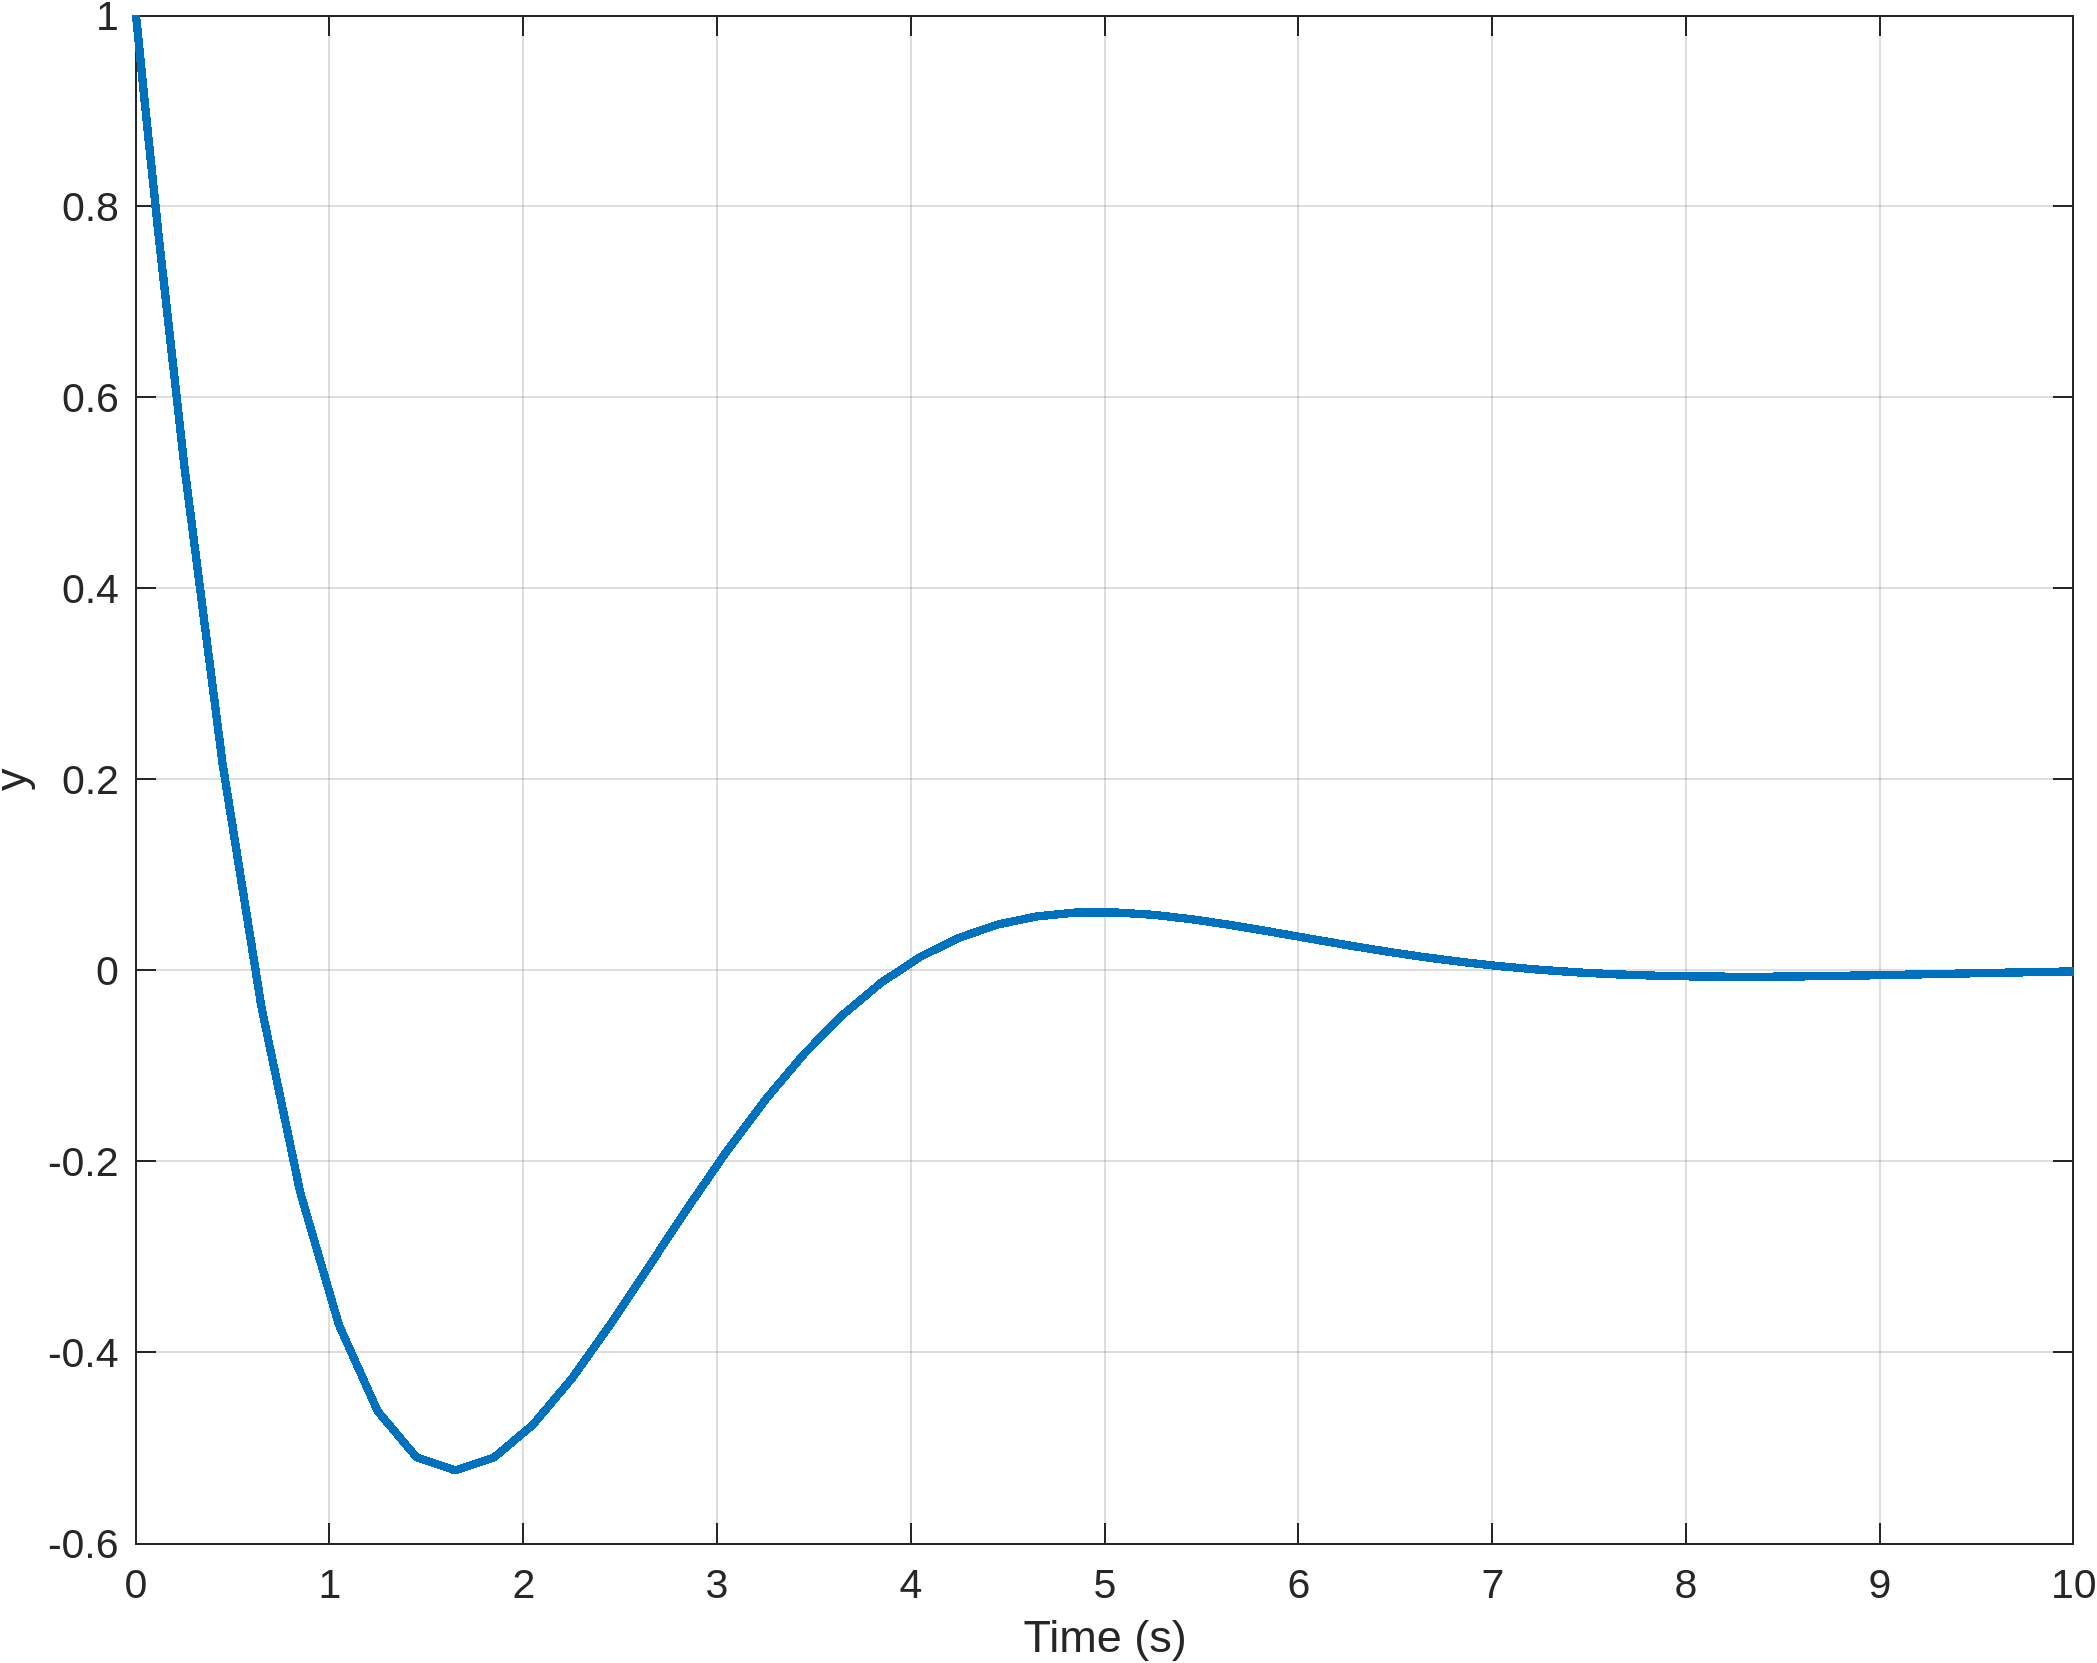
\includegraphics[width=0.8\textwidth]{figs/task_1_out_1.png}
    \caption{Свободное движение}
    \label{fig:task_1_out_1}
\end{figure}
\begin{figure}[H]
    \centering
    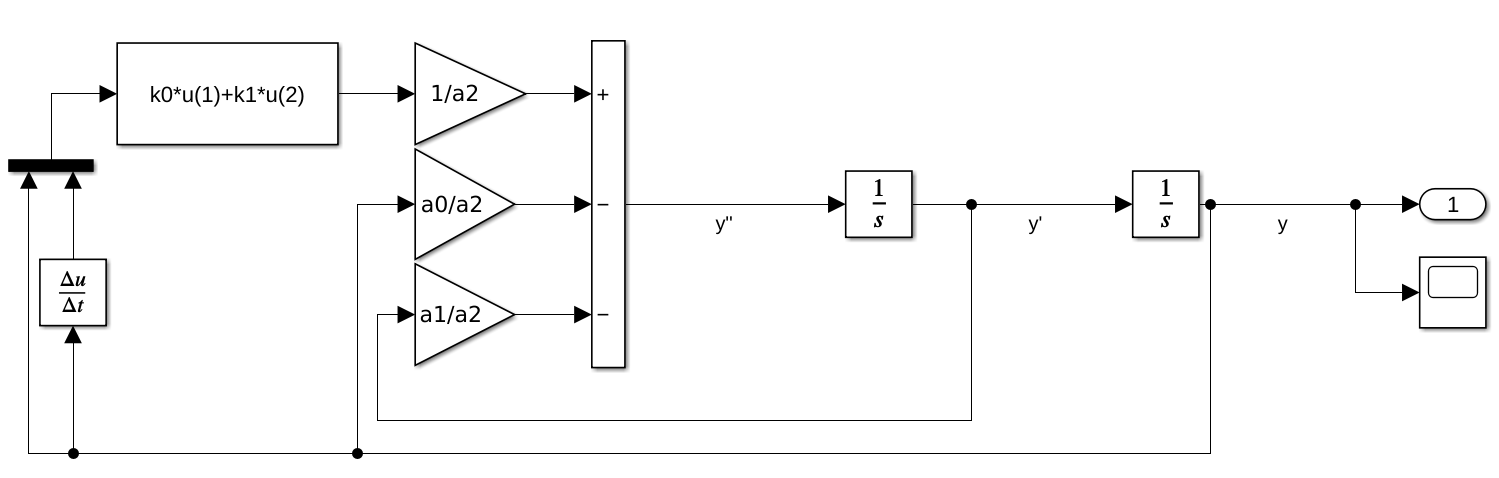
\includegraphics[width=1\textwidth]{figs/task_1_slx_1.png}
    \caption{Структурная схема для моделирования диффура с ПД регулятором}
    \label{fig:task_1_xls_1}
\end{figure}


\section{Задача стабилизации с реальным дифференцирующим звеном}

Модифицируем замкнутую систему из Задания 1, заменив аппроксимацию производной $\dot y(t)$
на передаточную функцию вида
\begin{equation*}
    W_{\text{р.дифф.}}(s)=\frac{s}{Ts+1},
\end{equation*}
используемую при этом структурную схему можно увидеть на рисунке \ref{fig:task_2_xls}.
\begin{figure}[H]
    \centering
    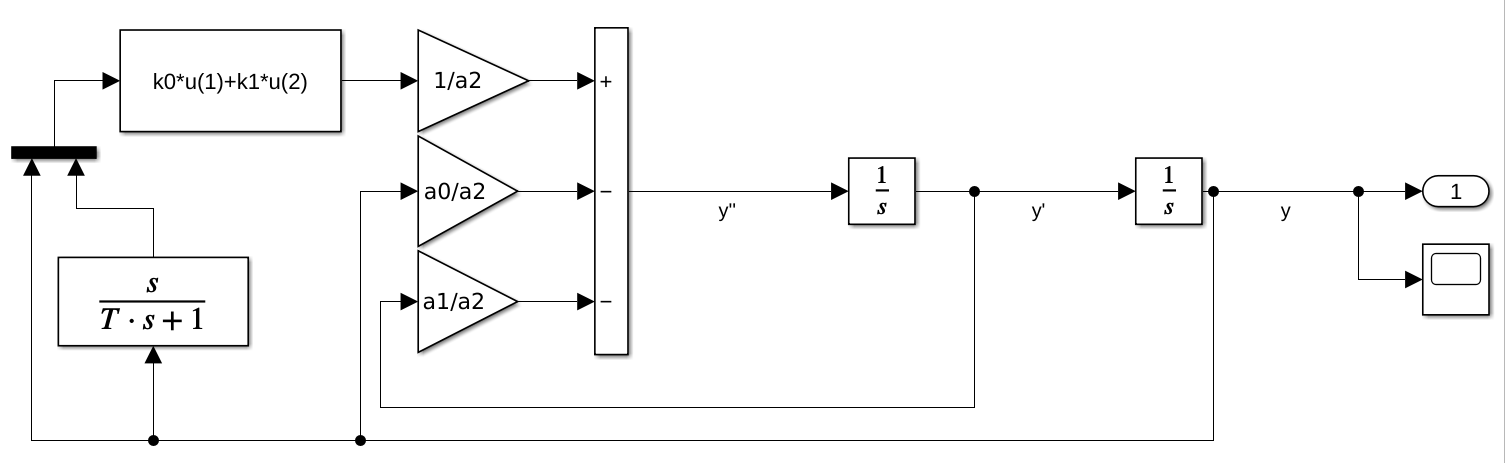
\includegraphics[width=1\textwidth]{figs/task_2_slx.png}
    \caption{Структурная схема для моделирования диффура с ручным приближением производной}
    \label{fig:task_2_xls}
\end{figure}
По результатам аналитических расчетов, которые можно посмотреть в конце
отчета, получилось что для асимптотической устойчивости
системы необходимо, чтобы $T$ была в интервале $(0;0.26)$, результаты 
моделирования для трех значений из этого интервала можно увидеть
на рисунке \ref{fig:task_2_out}. И чем меньше $T$, тем с меньшим
перерегулированием работает система, идеальное дифференцирующее звено сработало лучше.
\begin{figure}[H]
    \centering
    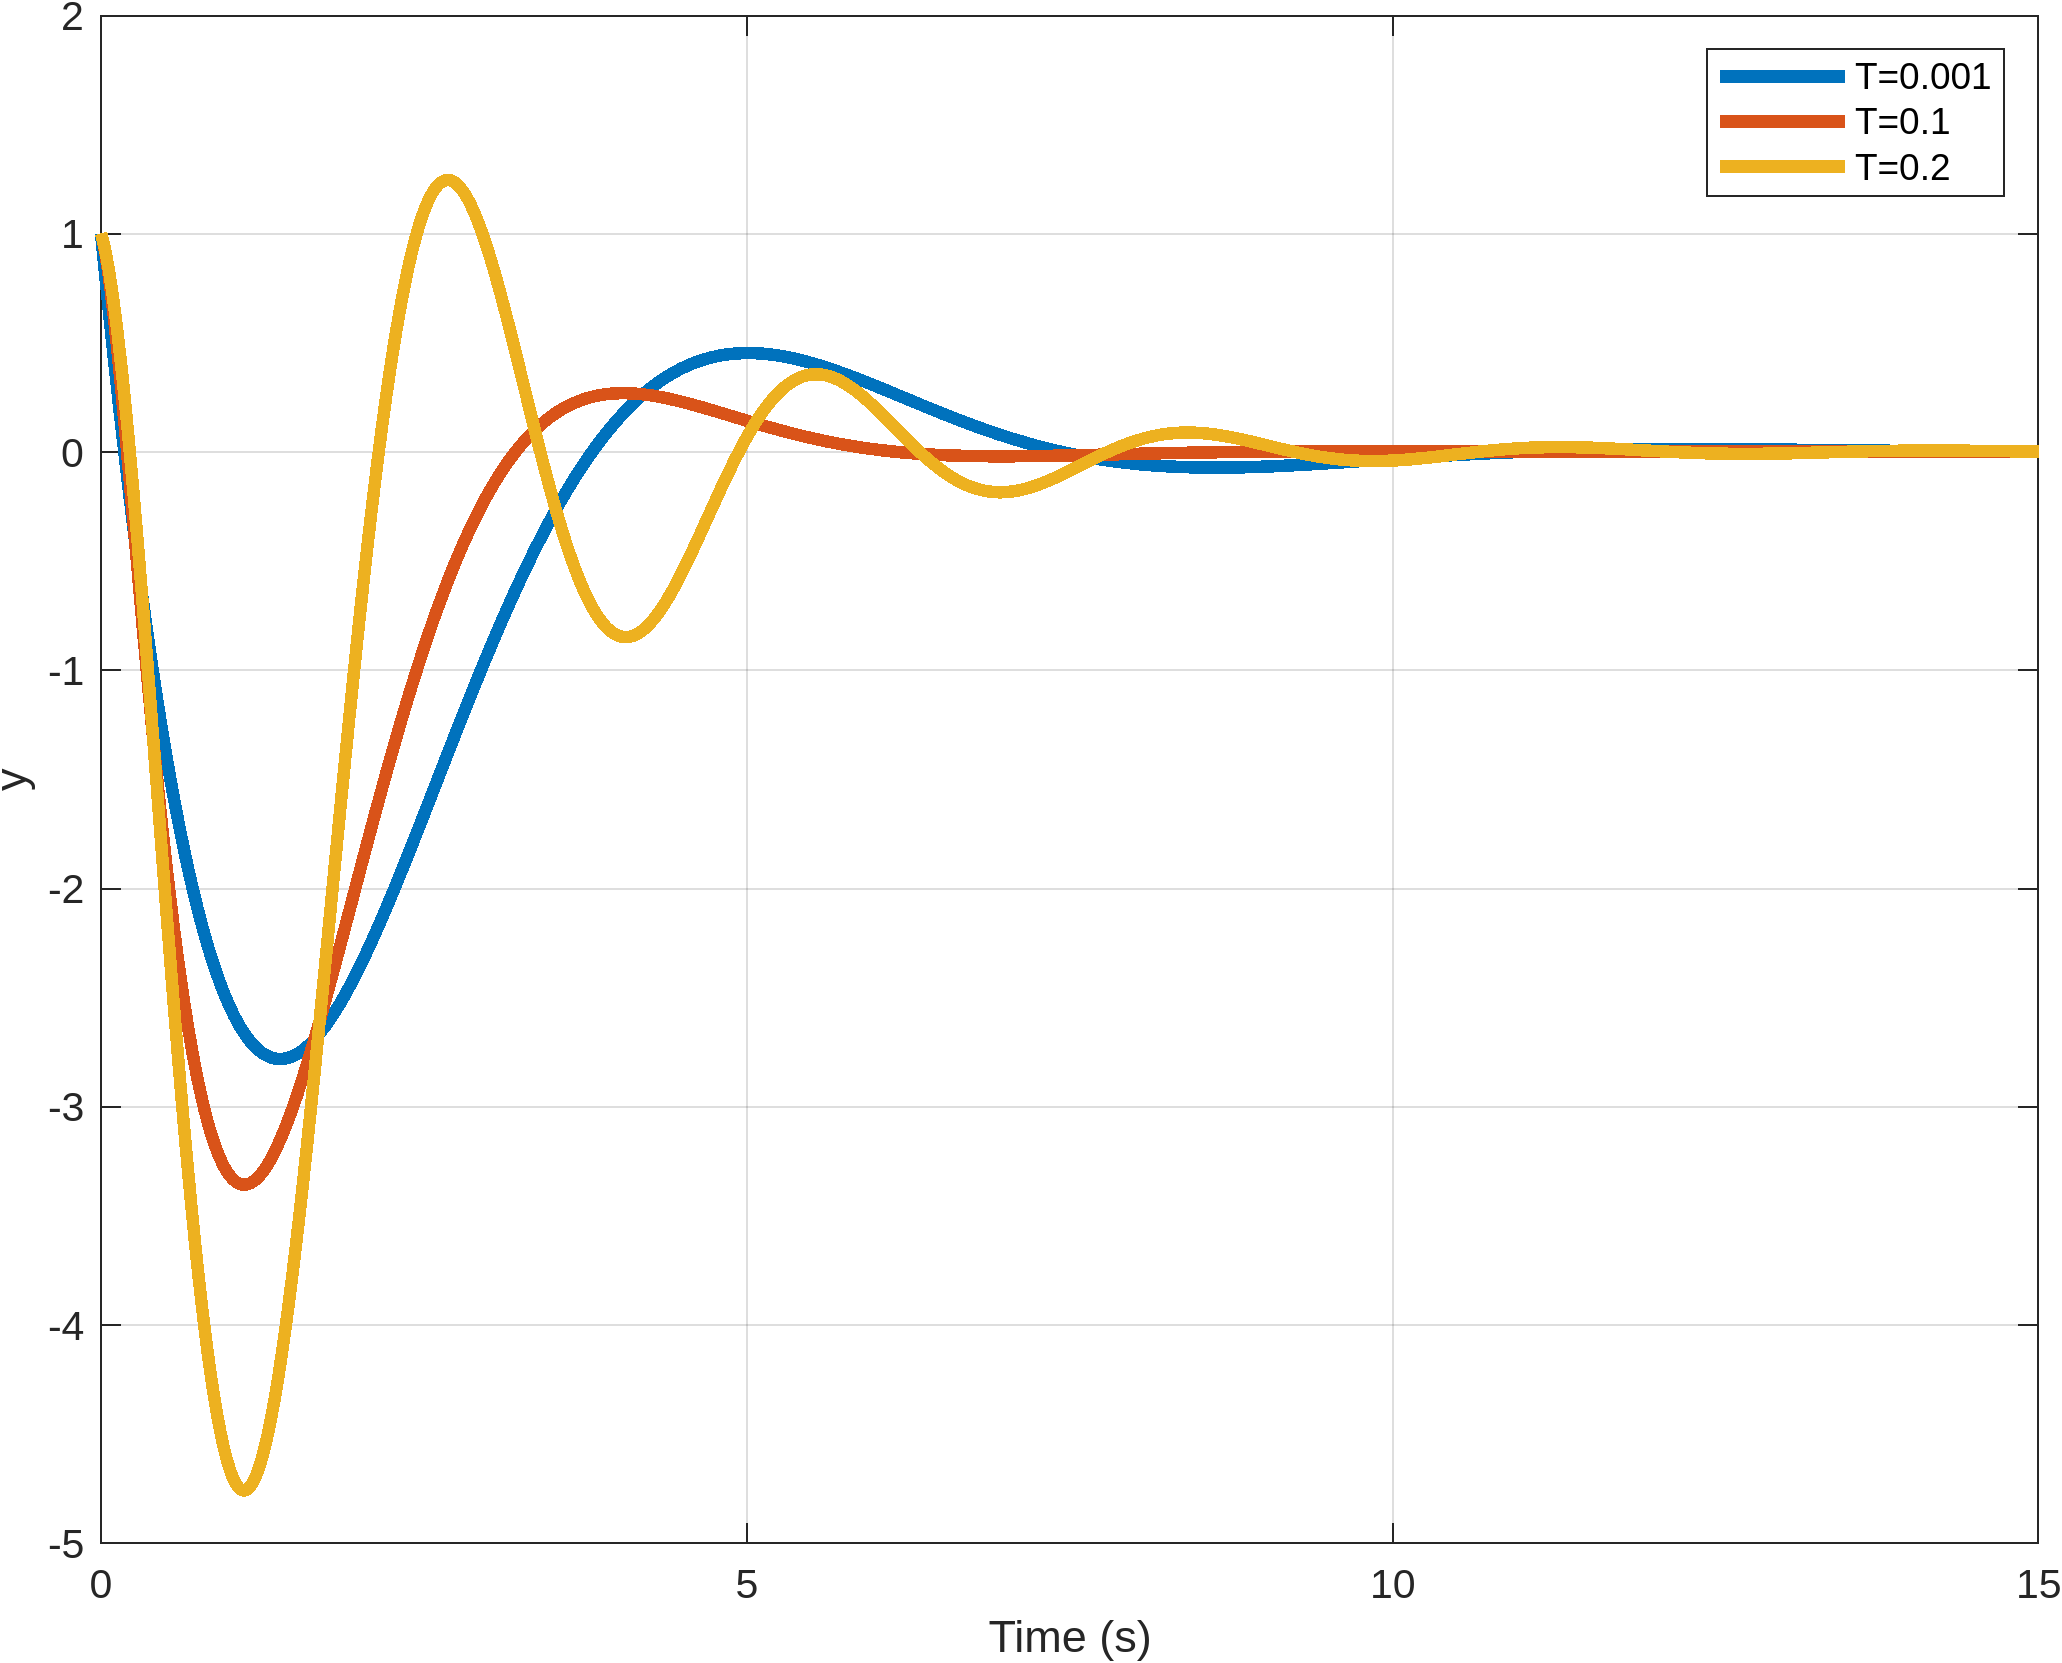
\includegraphics[width=0.9\textwidth]{figs/task_2_out.png}
    \caption{Графики выхода системы с управлением задания 2}
    \label{fig:task_2_out}
\end{figure}




\section{Задача слежения для системы с П регулятором}

Рассмотрим замкнутую систему, заданную структурной схемой на рисунке \ref{fig:task_3_xls}.
\begin{figure}[H]
    \centering
    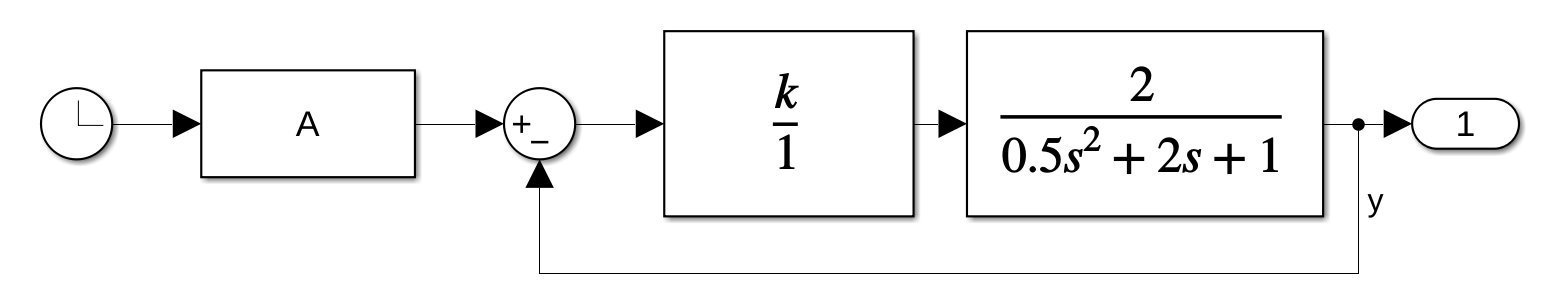
\includegraphics[width=1\textwidth]{figs/task_3_slx.png}
    \caption{Структурная схема для моделирования системы в общем виде}
    \label{fig:task_3_xls}
\end{figure}
В качестве регулятора используется П регулятор, а систему в ссответствии с вариантом
имеем
\begin{equation*}
    W(s)=\frac{2}{0.5s^2+2s+1}.
\end{equation*}
Найдем $k$ при которых система асимптотически устойчива, для этого найдем ПФ:
\begin{multline*}
    \underset{g\rightarrow e}{W} = \frac{1}{1+W(s)W_\text{рег}(s)}
    =\frac{1}{1+\frac{2k}{0.5s^2+2s+1}}=\frac{1}{\frac{0.5s^2+2s+1+2k}{0.5s^2+2s+1}}=\frac{0.5s^2+2s+1}{0.5s^2+2s+1+2k}.
\end{multline*}
По следствию из критерия Гурвица для асимптотической устойчивости системы нужно,
чтобы $k>-\frac{1}{2}$. Зададимся тремя $k$: $k_1=-0.25,\ k_2=5,\ k_3=10$.

Исследуем стационарный режим работы при $g(t)=A=1$. Чтобы аналитически вычислить
предельное значение ошибки для каждого значения $k$, найдем предел
\begin{multline*}
    \lim_{t\rightarrow\infty}e(t)=\lim_{s\rightarrow0}sE(s)=\lim_{s\rightarrow0}sG(s)\underset{g\rightarrow e}{W}(s)
    =\lim_{s\rightarrow0}\left(s\cdot\frac{A}{s}\cdot\frac{0.5s^2+2s+1}{0.5s^2+2s+1+2k}\right)
    =\frac{A}{1+2k}=\frac{1}{1+2k}.
\end{multline*}
Тогда найдем установившиеся значения для наших $k$ по формуле
\begin{equation*}
    y_\text{уст}=A-\frac{A}{1+2k},
\end{equation*}
которые можно увидеть в таблице \ref{tab:task_3_out}.
\begin{table}[H]
    \centering
    \caption{Установившиеся значения ошибок для системы с пропорциональным регулятором в стационарном режиме}
    \begin{tabular}{|c|c|}
        \hline
        $k_i$ & $y_\text{уст}$\\[2mm]
        -0.25 & -1.00 \\[2mm]
        5 & $\frac{10}{11}\approx0.91$ \\[2mm]
        10 & $\frac{20}{21}\approx0.95$ \\[2mm]
        \hline
    \end{tabular}
    \label{tab:task_3_out}
\end{table}

\begin{figure}[H]
    \centering
    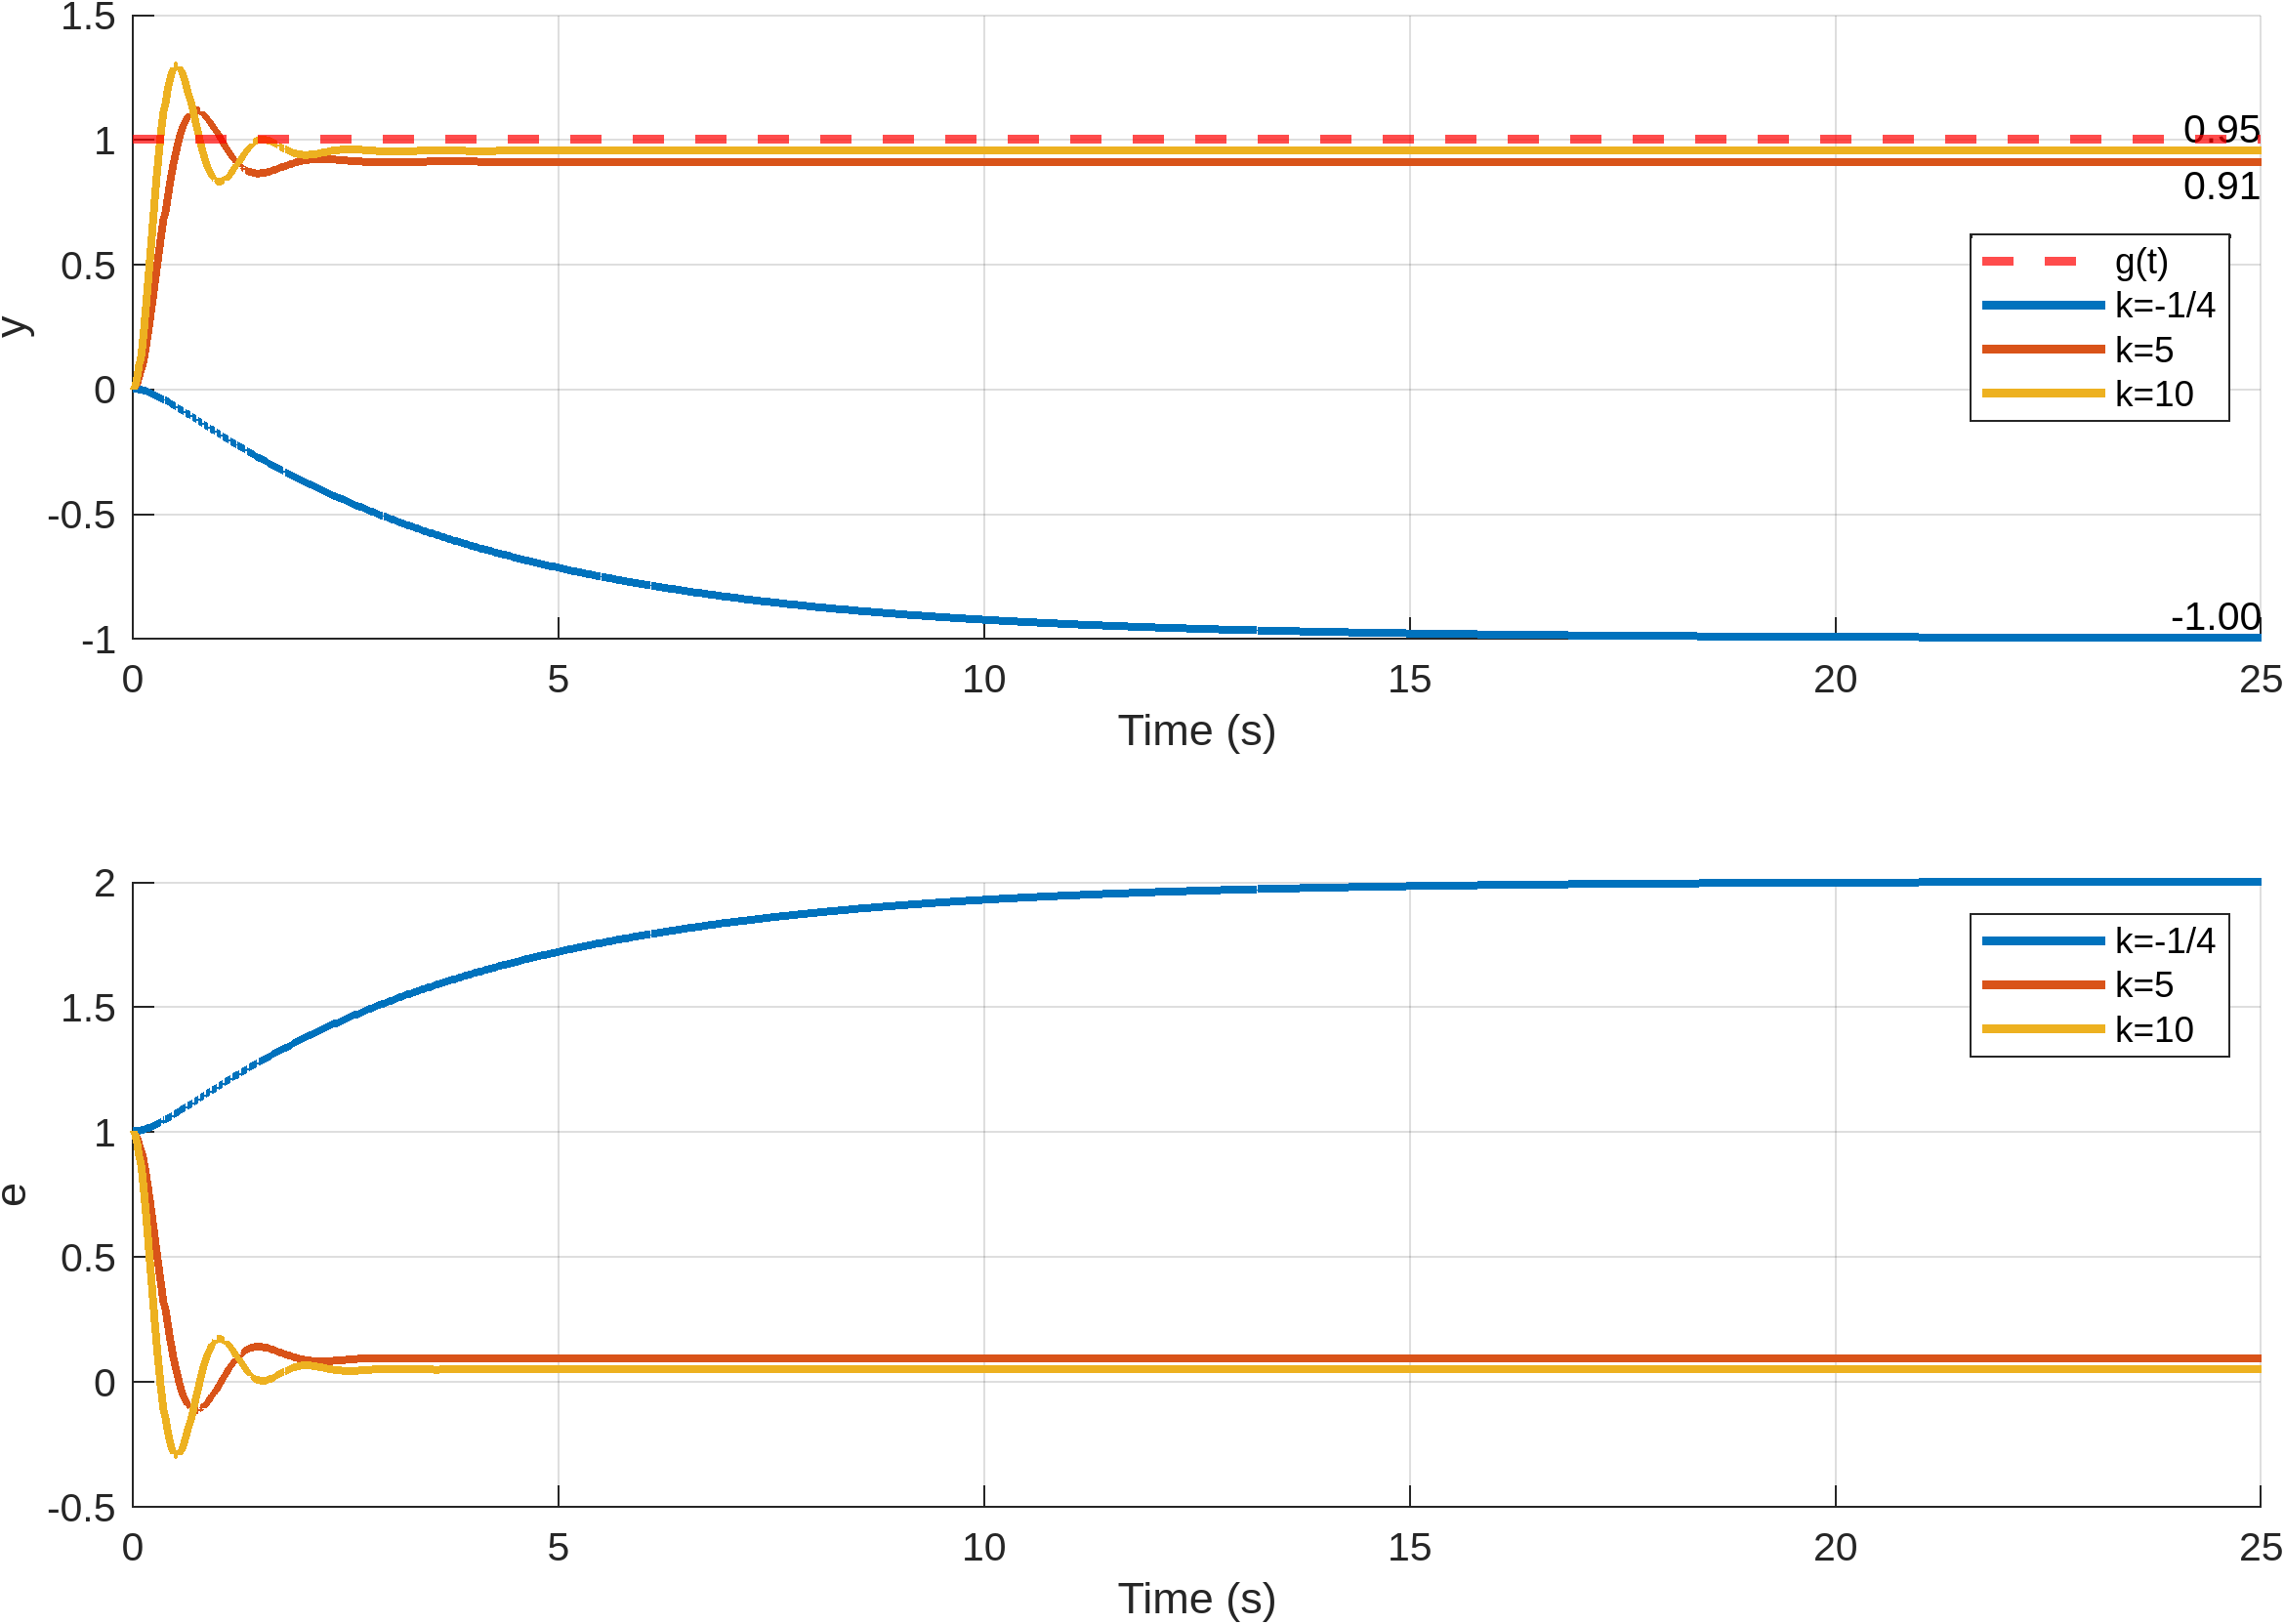
\includegraphics[width=1\textwidth]{figs/task_3_out.png}
    \caption{Графики выхода и ошибки системы с П регулятором в стационарном режиме работы}
    \label{fig:task_3_out}
\end{figure}
Посмотрим на рисунок \ref{fig:task_3_out} с симуляцией системы, в конце каждого графика
написано конечное значение, и, как видно, теория совпадает с симуляцией, имеем 
систему с астатизмом нулевого порядка и константный сигнал, поэтому разность
между сигналом $g$ и выходом константная разность после установления. Можно
видеть, что увеличение $k$ заставляет систему реагировать быстрее, система быстрее
достигает входного сигнала, но также увеличивается перерегулирование.

Исследуем режим движения с постоянной скоростью при $g(t) = Vt=2t$. 
\begin{figure}[H]
    \centering
    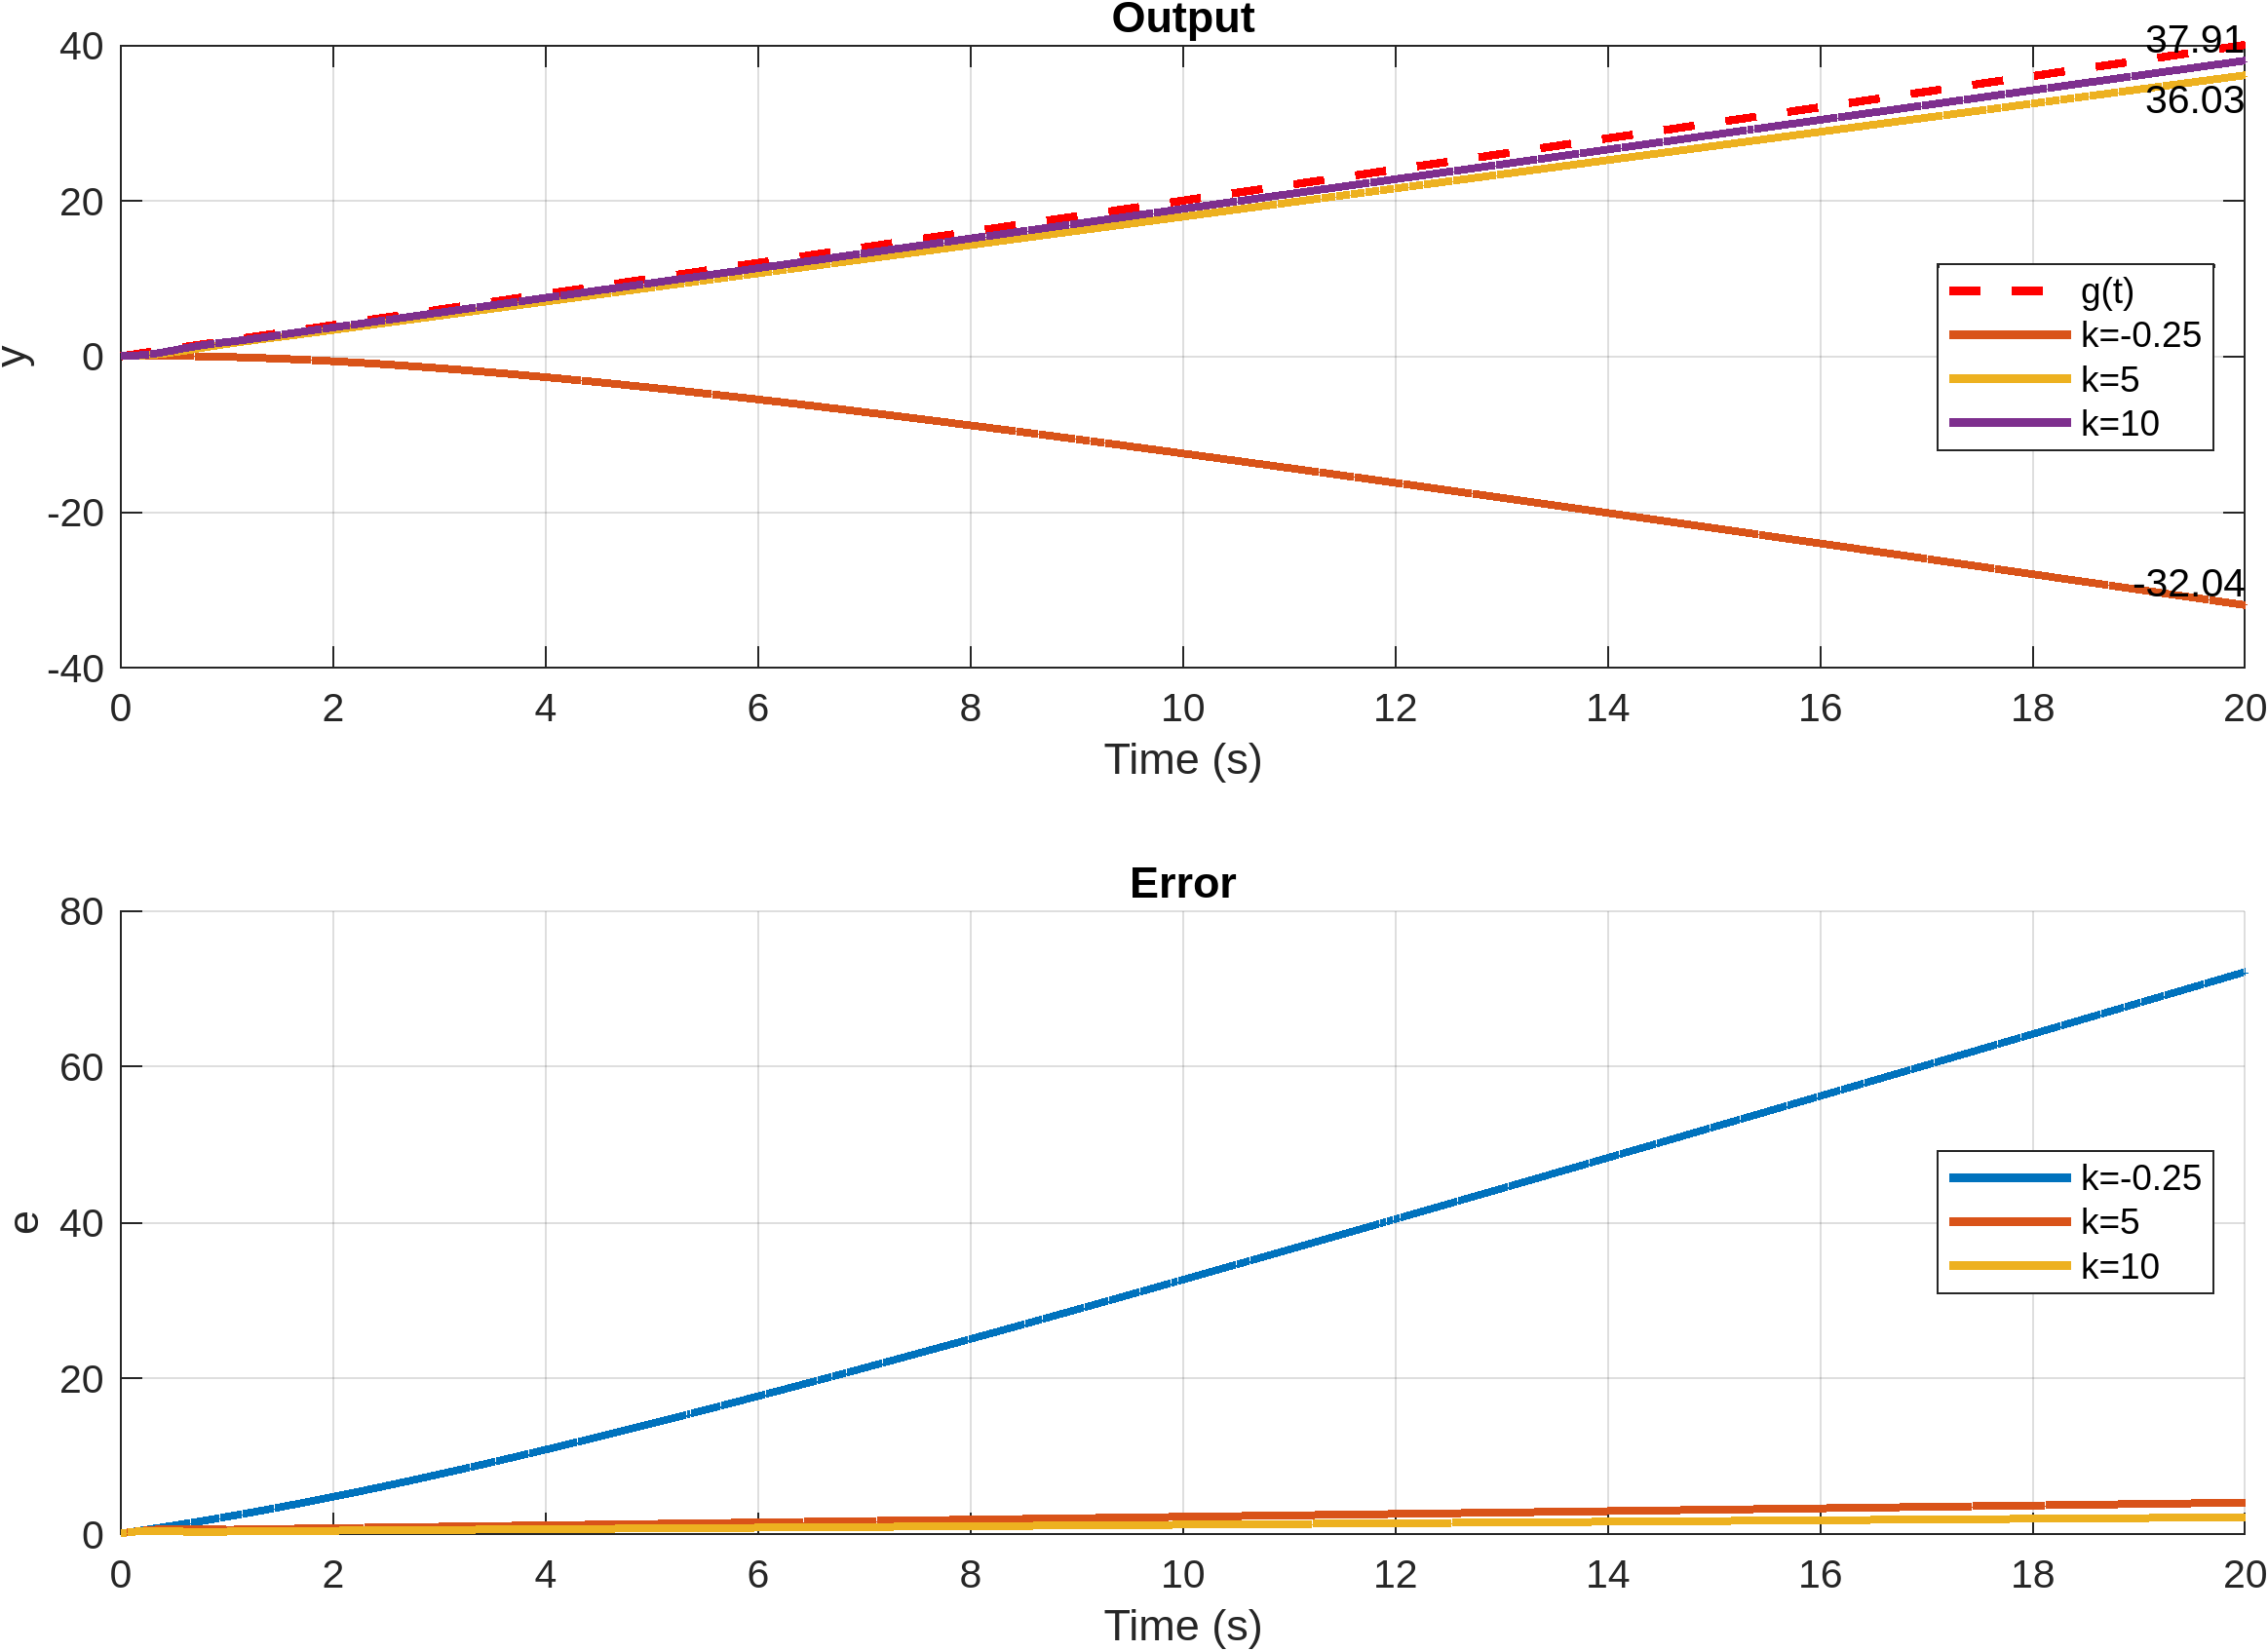
\includegraphics[width=1\textwidth]{figs/task_3_out_1.png}
    \caption{Графики выхода и ошибки системы с П регулятором в режиме движения с постоянной скоростью}
    \label{fig:task_3_out_1}
\end{figure}
Как можно видеть на рисунке \ref{fig:task_3_out_1} выход системы не успевает за сигналом,
и разность между ними увеличивается со временем, что и ожидается от системы с астатизмом
нулевого порядка и входного сигнала в виде многочлена первого порядка. Из рисунка
можно заметить, что чем больше $k$, тем ближе выход системы к входному сигналу.


\section{Задача слежения для системы с И регулятором}

Рассмотрим замкнутую систему, заданную структурной схемой на рисунке \ref{fig:task_3_xls},
но регулятор теперь будет таким
\begin{equation*}
    H(s)=\frac{k}{s}
\end{equation*}
--- интегральный регулятор. Исследуем систему, чтобы найти при каких $k$ она асимптотически
устойчива. ПФ по ошибке
\begin{equation*}
    \underset{g\rightarrow e}{W}(s)=\frac{1}{1+\frac{2k}{s(0.5s^2+2s+1)}}=\frac{1}{\frac{0.5s^3+2s^2+s+2k}{s(0.5s^2+2s+1)}}=\frac{s(0.5s^2+2s+1)}{0.5s^3+2s^2+s+2k}.
\end{equation*}
Тогда, используя следствие из критерия Гурвица, для асимптотической устойчивости системы
необходимо, чтобы $0<k<1$. Выберем $k$: $k_1=0.1,\ k_2=0.5,\ k_3=0.9$.
Как можно видеть по ПФ, система имеет первый порядок астатизма, откуда следует, что при слежении за
константным сигналом ($g(t)=A$) установившаяся ошибка должна быть равна нулю, подтвердим это расчетами:
\begin{multline*}
    \lim_{t\rightarrow\infty}e(t)
    =\lim_{s\rightarrow0}sE(s)
    =\lim_{s\rightarrow0}sG(s)\underset{g\rightarrow e}{W}(s)
    =\lim_{s\rightarrow0}\left(s\cdot A\cdot\frac{s(0.5s^2+2s+1)}{0.5s^3+2s^2+s+2k}\right)
    =0,
\end{multline*}
вывод был верным, для движения с постоянной 
скорость ($g(t)=Vt$) установившаяся ошибка будет константой, подтвердим это расчетами:
\begin{multline*}
    \lim_{t\rightarrow\infty}e(t)
    =\lim_{s\rightarrow0}sE(s)
    =\lim_{s\rightarrow0}sG(s)\underset{g\rightarrow e}{W}(s)
    =\lim_{s\rightarrow0}\left(s\cdot\frac{V}{s^2}\cdot\frac{s(0.5s^2+2s+1)}{0.5s^3+2s^2+s+2k}\right)
    =\frac{V}{2k}=\frac{1}{k},
\end{multline*}
вывод был верным, расчитанные установившиеся значения можно увидеть в таблице \ref{tab:task_4_out},
если следить за входным сигналом с 
постоянным ускорением ($g(t)=\frac{at^2}{2}$), то ошибка будет постоянно увеличиваться, подтвердим это расчетами:
\begin{multline*}
    \lim_{t\rightarrow\infty}e(t)
    =\lim_{s\rightarrow0}sE(s)
    =\lim_{s\rightarrow0}sG(s)\underset{g\rightarrow e}{W}(s)
    =\lim_{s\rightarrow0}\left(s\cdot\frac{a}{s^3}\cdot\frac{s(0.5s^2+2s+1)}{0.5s^3+2s^2+s+2k}\right)
    =\infty.
\end{multline*}

\begin{table}[H]
    \centering
    \caption{Установившиеся значения ошибок для системы с интегральным регулятором в режиме движения с постоянной скоростью (см. рис \ref{fig:task_4_out_linear})}
    \begin{tabular}{|c|c|}
        \hline
        $k_i$ & $e_\text{уст}$\\[2mm]
        0.1 & 10.00 \\[2mm]
        0.5 & 2.00 \\[2mm]
        0.9 & 1.11 \\[2mm]
        \hline
    \end{tabular}
    \label{tab:task_4_out}
\end{table}
Результаты моделирования можно видеть на рисунках \ref{fig:task_4_out_constant}, 
\ref{fig:task_4_out_linear} и \ref{fig:task_4_out_quadratic}. Все сходится с выводами выше.

\begin{figure}[H]
    \centering
    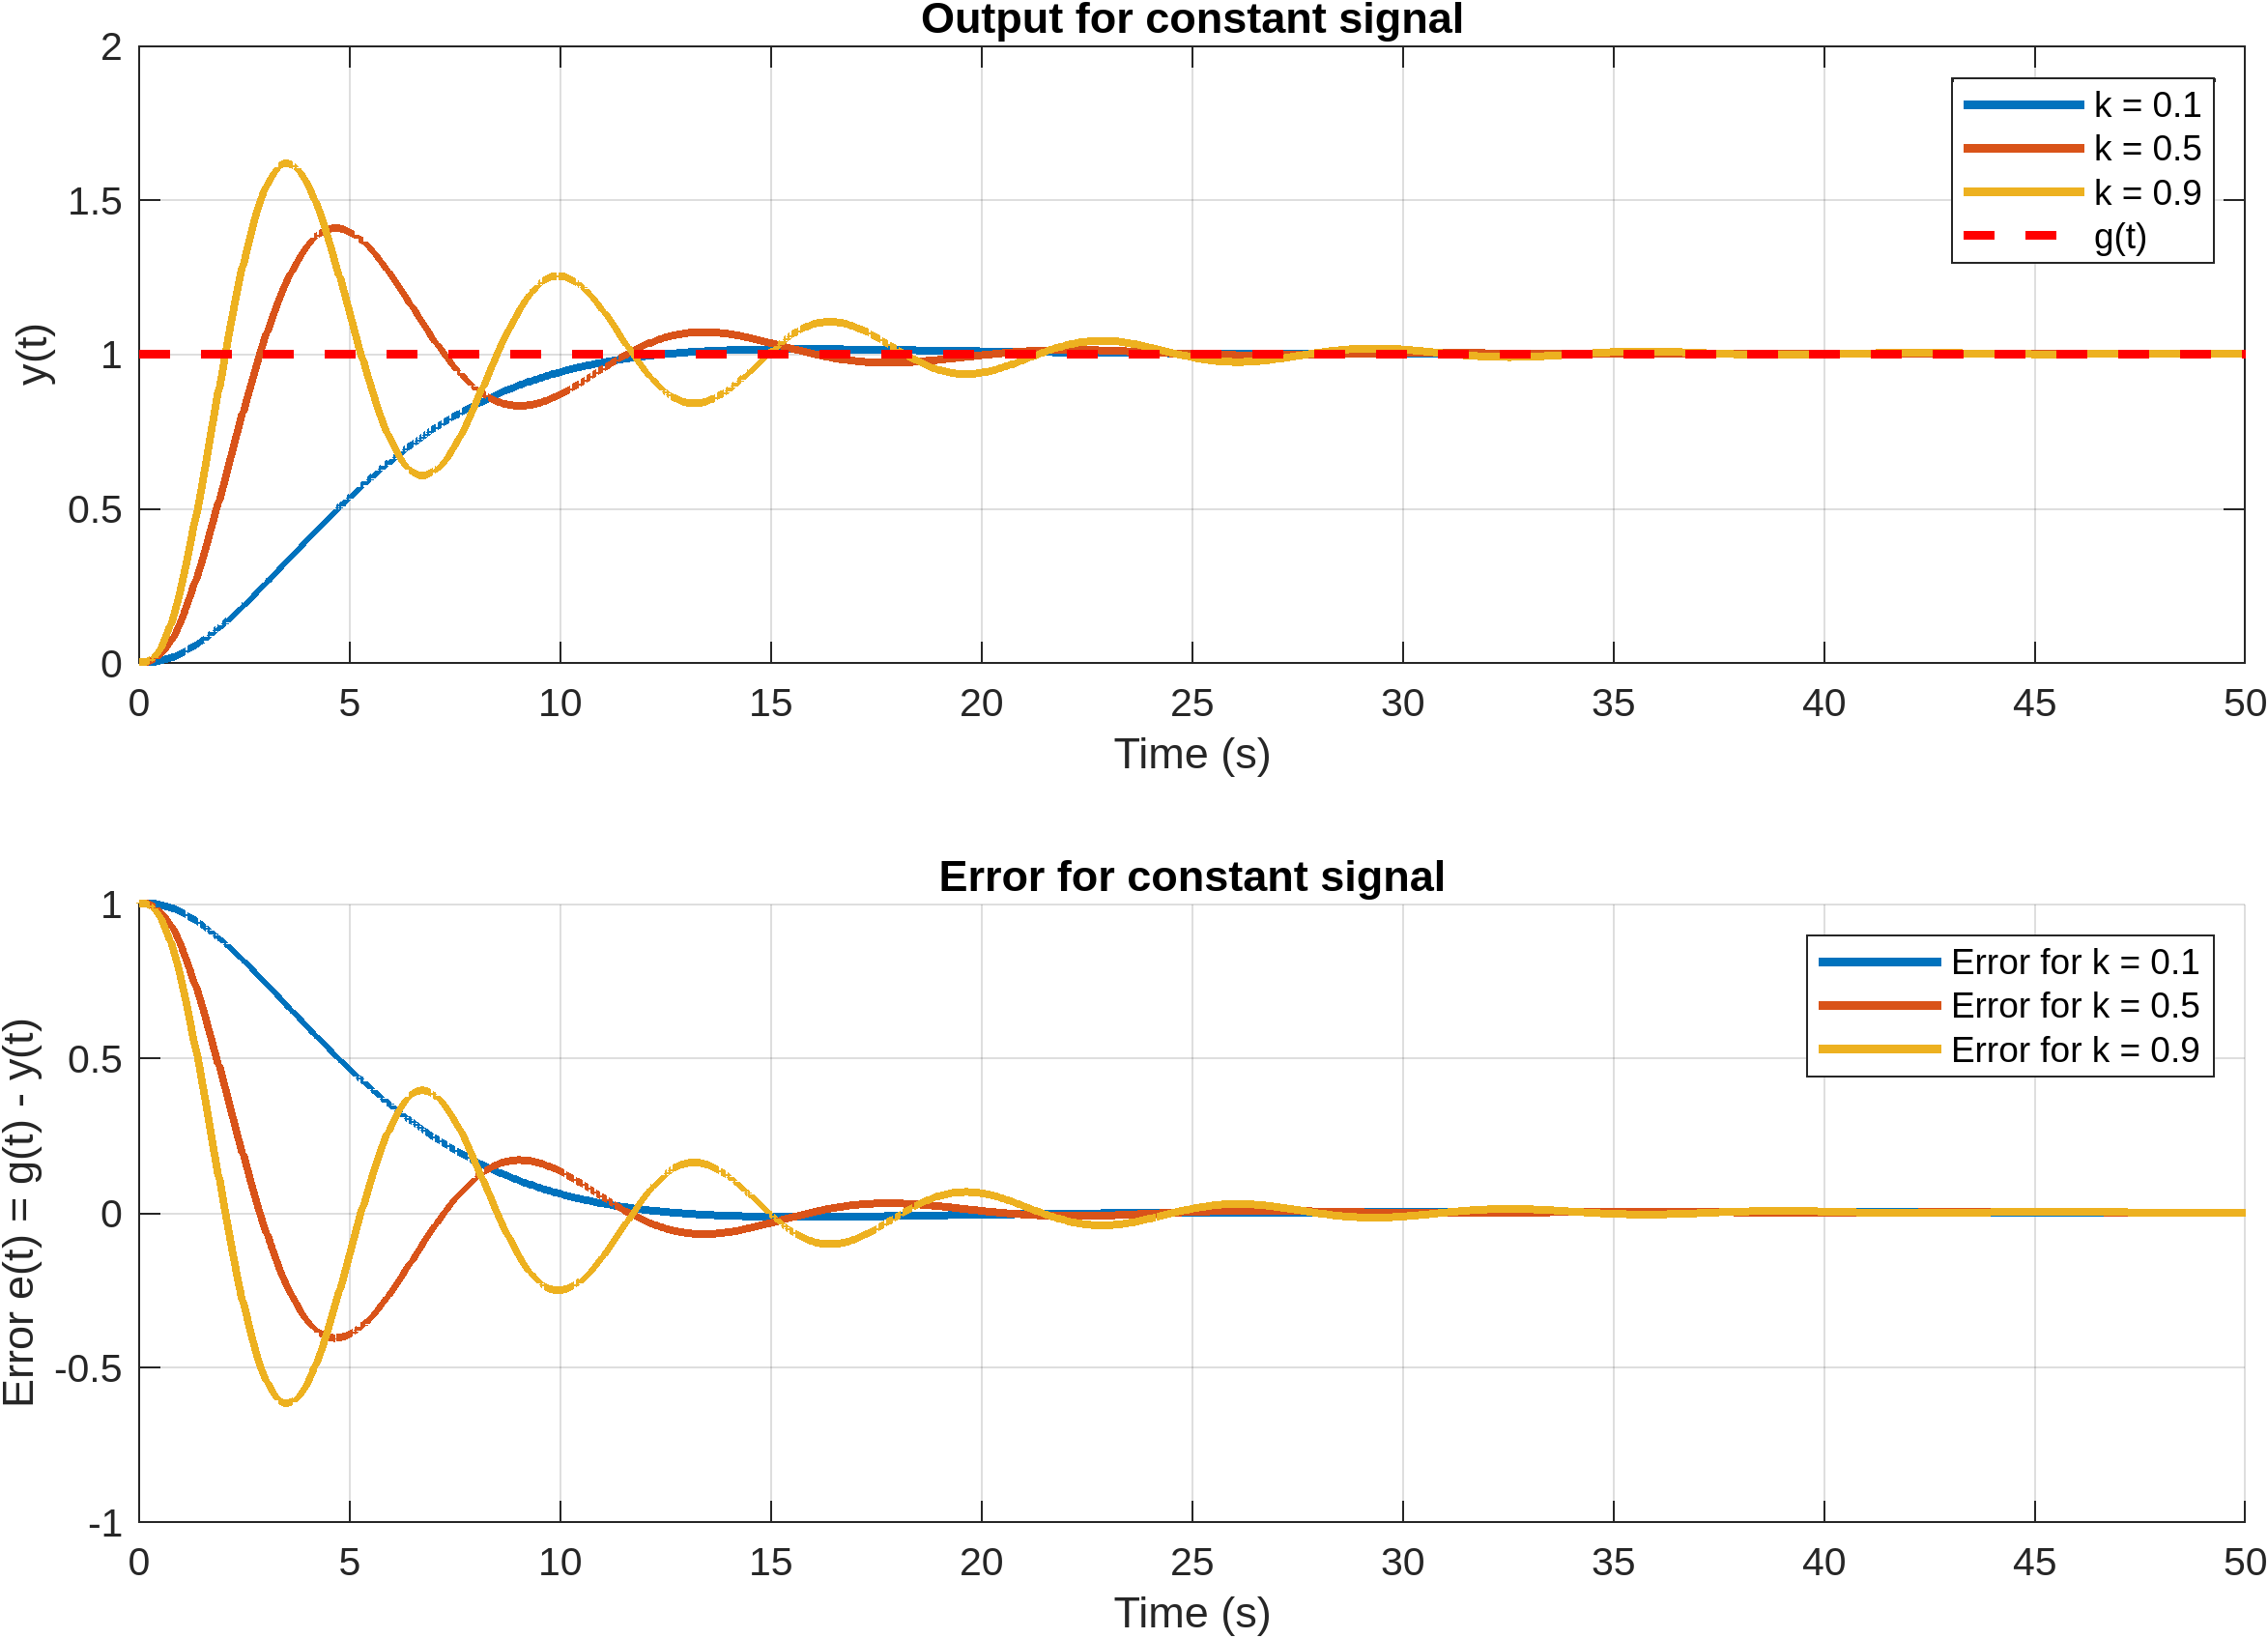
\includegraphics[width=0.9\textwidth]{figs/task_4_out_constant.png}
    \caption{Графики выхода и ошибки системы с интегральным регулятором в стационарном режиме работы}
    \label{fig:task_4_out_constant}
\end{figure}
\begin{figure}[H]
    \centering
    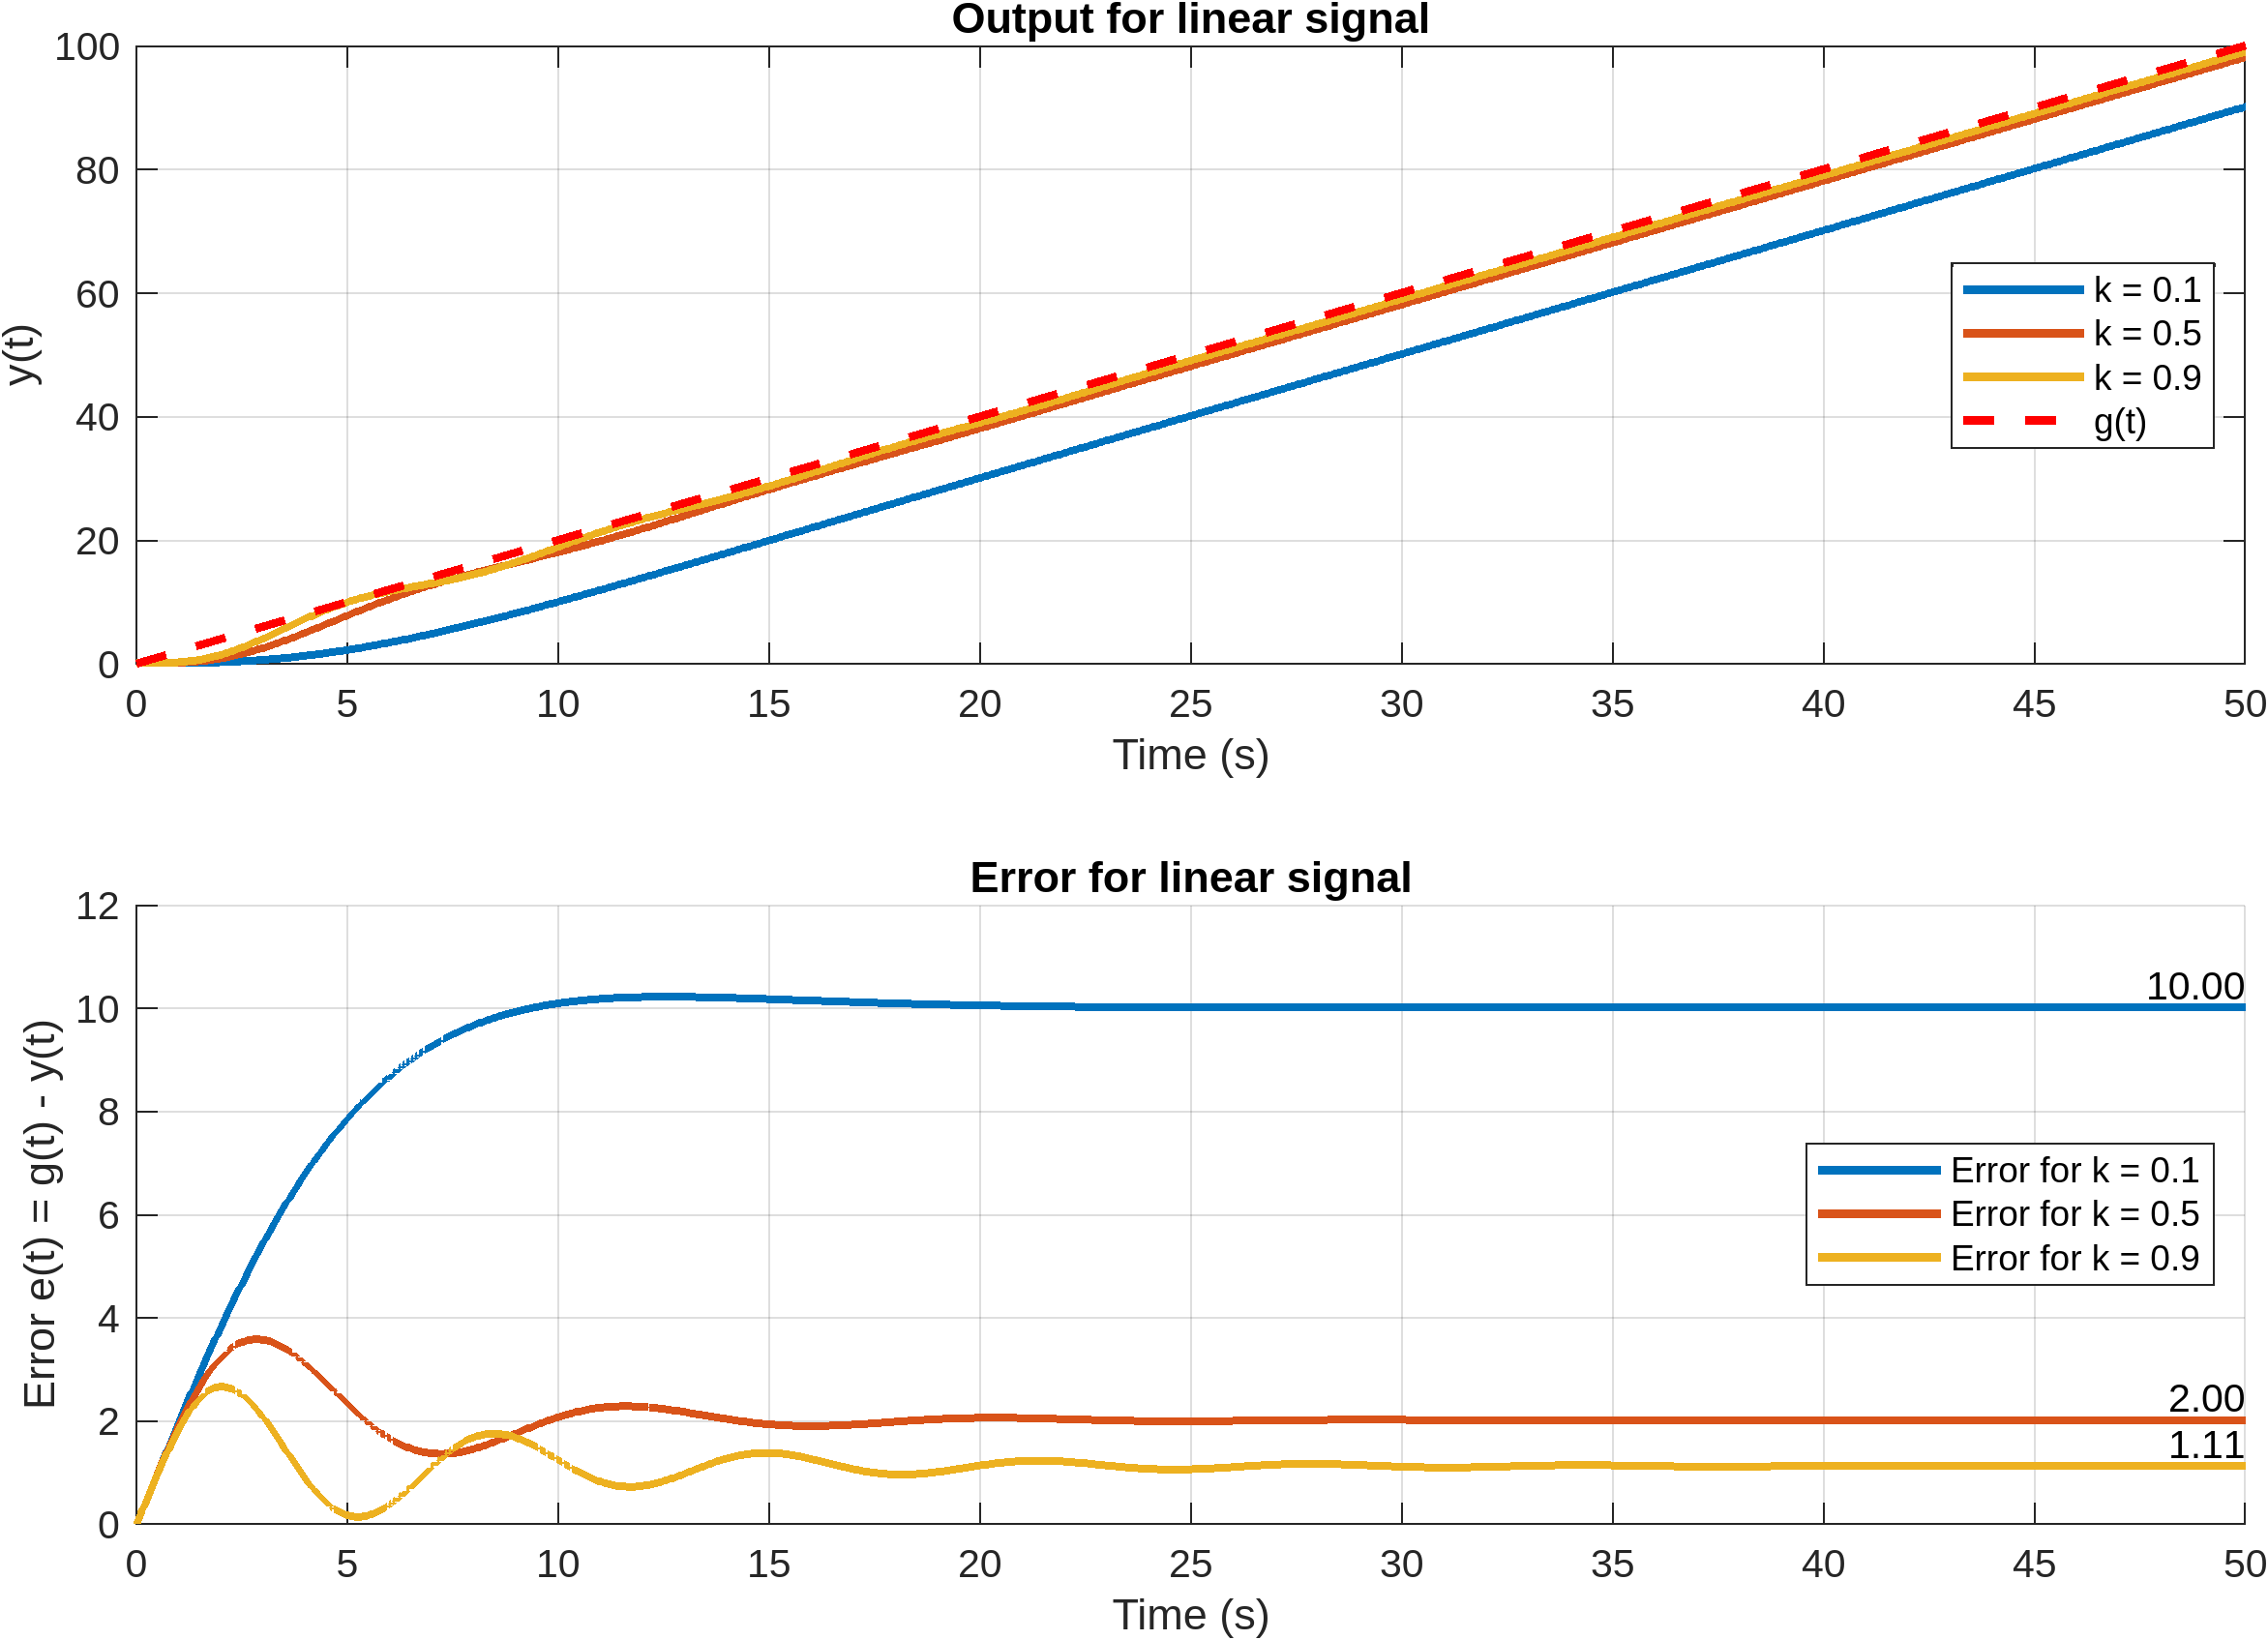
\includegraphics[width=0.85\textwidth]{figs/task_4_out_linear.png}
    \caption{Графики выхода и ошибки системы с интегральным регулятором в режиме движения с постоянной скоростью}
    \label{fig:task_4_out_linear}
\end{figure}
\begin{figure}[H]
    \centering
    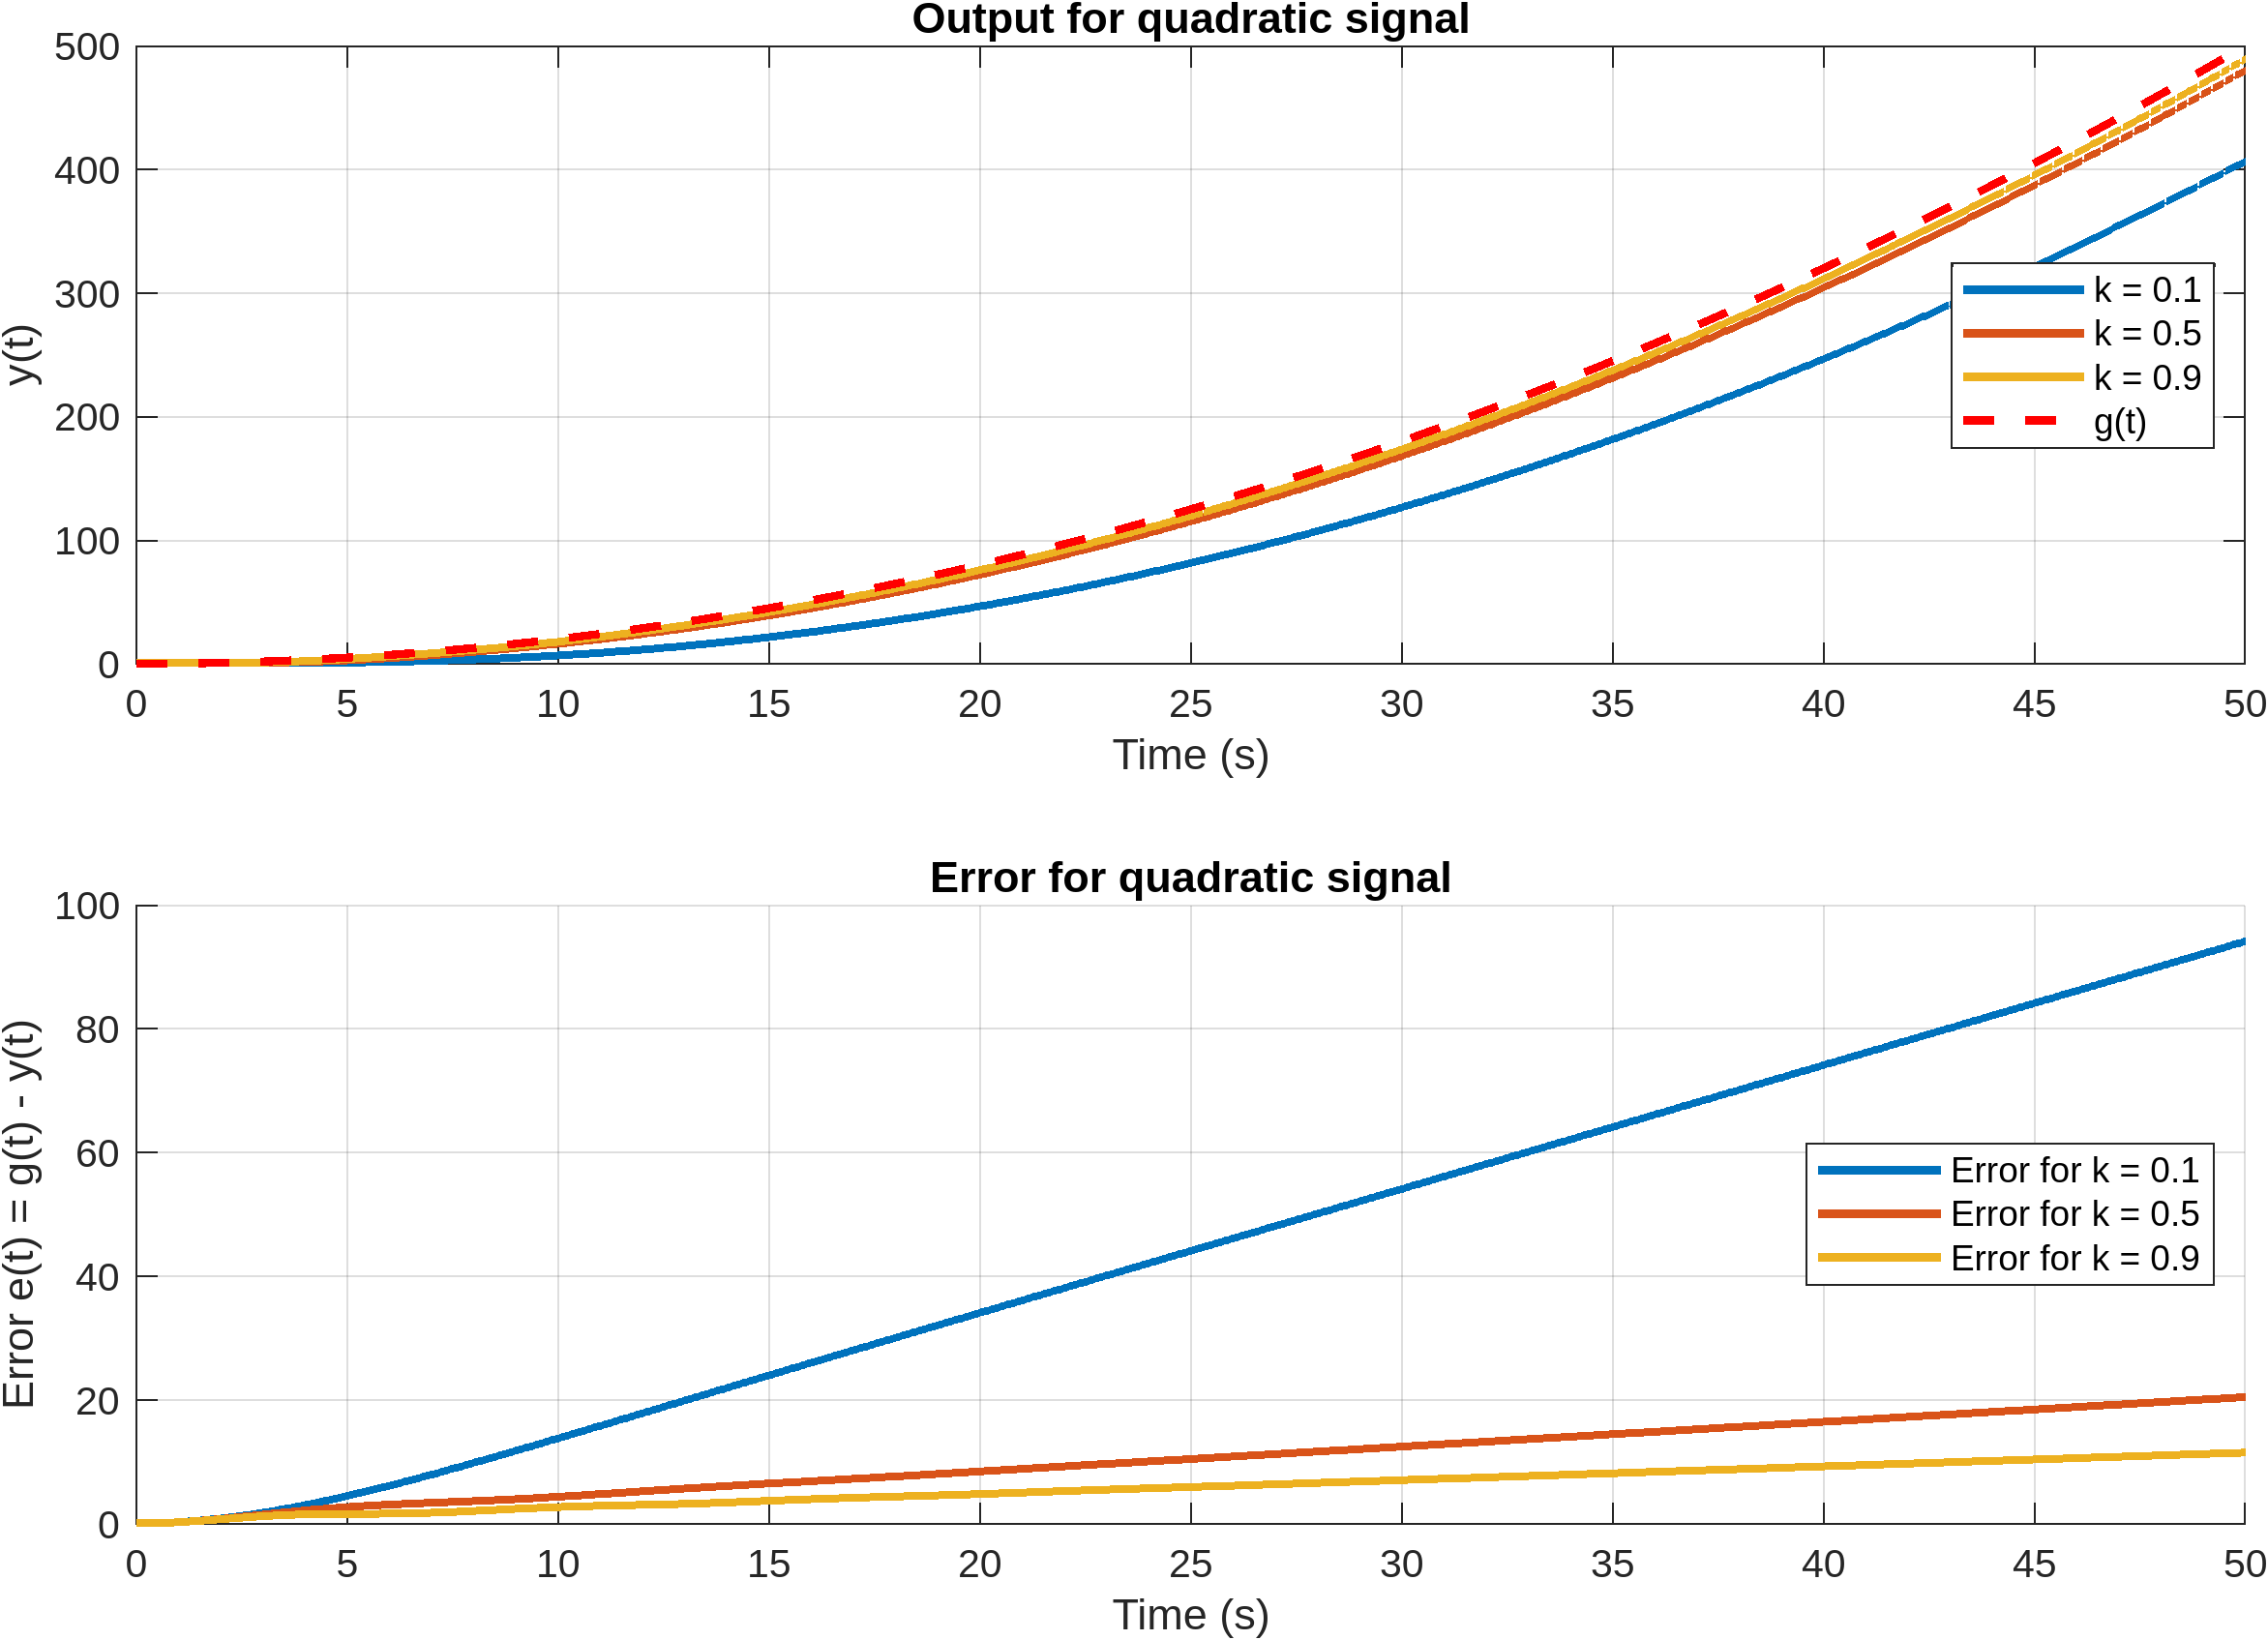
\includegraphics[width=0.9\textwidth]{figs/task_4_out_quadratic.png}
    \caption{Графики выхода и ошибки системы с интегральным регулятором в режиме движения с постоянным ускорением}
    \label{fig:task_4_out_quadratic}
\end{figure}



\section{Задача слежения для системы с ПИ регулятором}

Рассмотрим замкнутую систему, заданную структурной схемой на рисунке \ref{fig:task_3_xls},
но изменим регулятор
\begin{equation*}
    H(s)=\frac{{k_i}}{s}+k_p=\frac{k_ps+k_i}{s},
\end{equation*}
\begin{multline*}
    \underset{g\rightarrow e}{W}(s)
    =\frac{1}{1+\frac{2(k_ps+k_i)}{s(0.5s^2+2s+1)}}
    =\frac{1}{\frac{0.5s^3+2s^2+s+2k_ps+2k_i}{s(0.5s^2+2s+1)}}
    =\frac{s(0.5s^2+2s+1)}{0.5s^3+2s^2+(1+2k_p)s+2k_i}.
\end{multline*}
Тогда, используя следствие из критерия Гурвица, для асимптотической устойчивости системы
необходимо, чтобы 
\begin{equation*}
    \begin{cases}
        k_i>0,\\
        k_p>-\frac{1}{2},\\
        2k_p+1>k_i.
    \end{cases}
\end{equation*} 
Выберем $k_p$: $k_{p1}=5,\ k_{p2}=10,\ k_{p3}=20$;
$k_i$: $k_{i1}=0.1,\ k_{i2}=2,\ k_{i3}=6$; тогда все пары $(k_p,k_i)$ будут
асимптотически устойчивы.

Аналитически найдем установившуюся ошибку для слежения за сигналом с постоянной скоростью:
\begin{multline*}
    \lim_{t\rightarrow\infty}e(t)
    =\lim_{s\rightarrow0}sE(s)=\lim_{s\rightarrow0}sG(s)\underset{g\rightarrow e}{W}(s)
    =\lim_{s\rightarrow0}\left(s\cdot\frac{V}{s^2}\cdot\frac{s(0.5s^2+2s+1)}{0.5s^3+2s^2+(1+2k_p)s+2k_i}\right)
    =\frac{V}{2k_i}=\frac{1}{k_i}.
\end{multline*}

Проведем моделирование для слежения за сигналом с постоянной скоростью и гармоническим
сигналом, результаты можно видеть на рисунках \ref{fig:task_5_out_linear}, \ref{fig:task_5_out_1_linear} и \ref{fig:task_5_out_harmonic}.
В таблицу \ref{tab:task_5_out} занесены установшиеся значения после 1000 секунд
моделирования для линейного сигнала. Они сходятся с аналитическими значениями.

\begin{table}[H]
    \centering
    \caption{Установившиеся значения $y$ и аналитические значения для линейного входного сигнала}
    \begin{tabular}{|c|c|c|c|}
        \hline
        $k_p$ & $k_i$ & Экспериментальное $y_{\text{уст}}$ & Аналитическое $y_{\text{уст}}$\\ \hline
        5 & 0.1 & 9.9999 & 10.0000 \\
        5 & 2.0 & 0.5000 & 0.5000 \\
        5 & 6.0 & 0.1667 & 0.1667 \\
        10 & 0.1 & 9.9993 & 10.0000 \\
        10 & 2.0 & 0.5000 & 0.5000 \\
        10 & 6.0 & 0.1667 & 0.1667 \\
        20 & 0.1 & 9.9247 & 10.0000 \\
        20 & 2.0 & 0.5000 & 0.5000 \\
        20 & 6.0 & 0.1667 & 0.1667 \\ \hline
    \end{tabular}
    \label{tab:task_5_out}
\end{table}

Симуляцию при линейном входе можно видеть на рисунках \ref{fig:task_5_out_linear_ki0.1}, \ref{fig:task_5_out_linear_ki2.0} и \ref{fig:task_5_out_linear_ki6.0},
при гармоническом входе - на рисунках \ref{fig:task_5_out_harmonic_ki0.1}, \ref{fig:task_5_out_harmonic_ki2.0} и \ref{fig:task_5_out_harmonic_ki6.0},
так же, поскольку на графиках при линейном входе выходы сливаются, на рисунках \ref{fig:task_5_output_ki_0.1}, \ref{fig:task_5_output_ki_2.0} и \ref{fig:task_5_output_ki_6.0}
выходы рассмотрены при малых $t$.

Эспериментальное установившееся значения при линейном входе были записаны в таблицу \ref{tab:task_5_out}, наибольшую установившуюся ошибку
имеют три набора пар (см. Рис. \ref{fig:task_5_out_linear_ki0.1}) $k_{p1}=5,\ k_{i1}=0.1,\ k_{p2}=10,\ k_{i2}=0.1,\ k_{p3}=20,\ k_{i3}=0.1$,
им потребовалось больше всего времени на установление.
их объединяет малый $k_i$. При слежении за гармоническим сигналом регулятор справился очень плохо
при любых рассмотренных коэффициентах.

% Линейный сигнал
\begin{figure}[H]
    \centering
    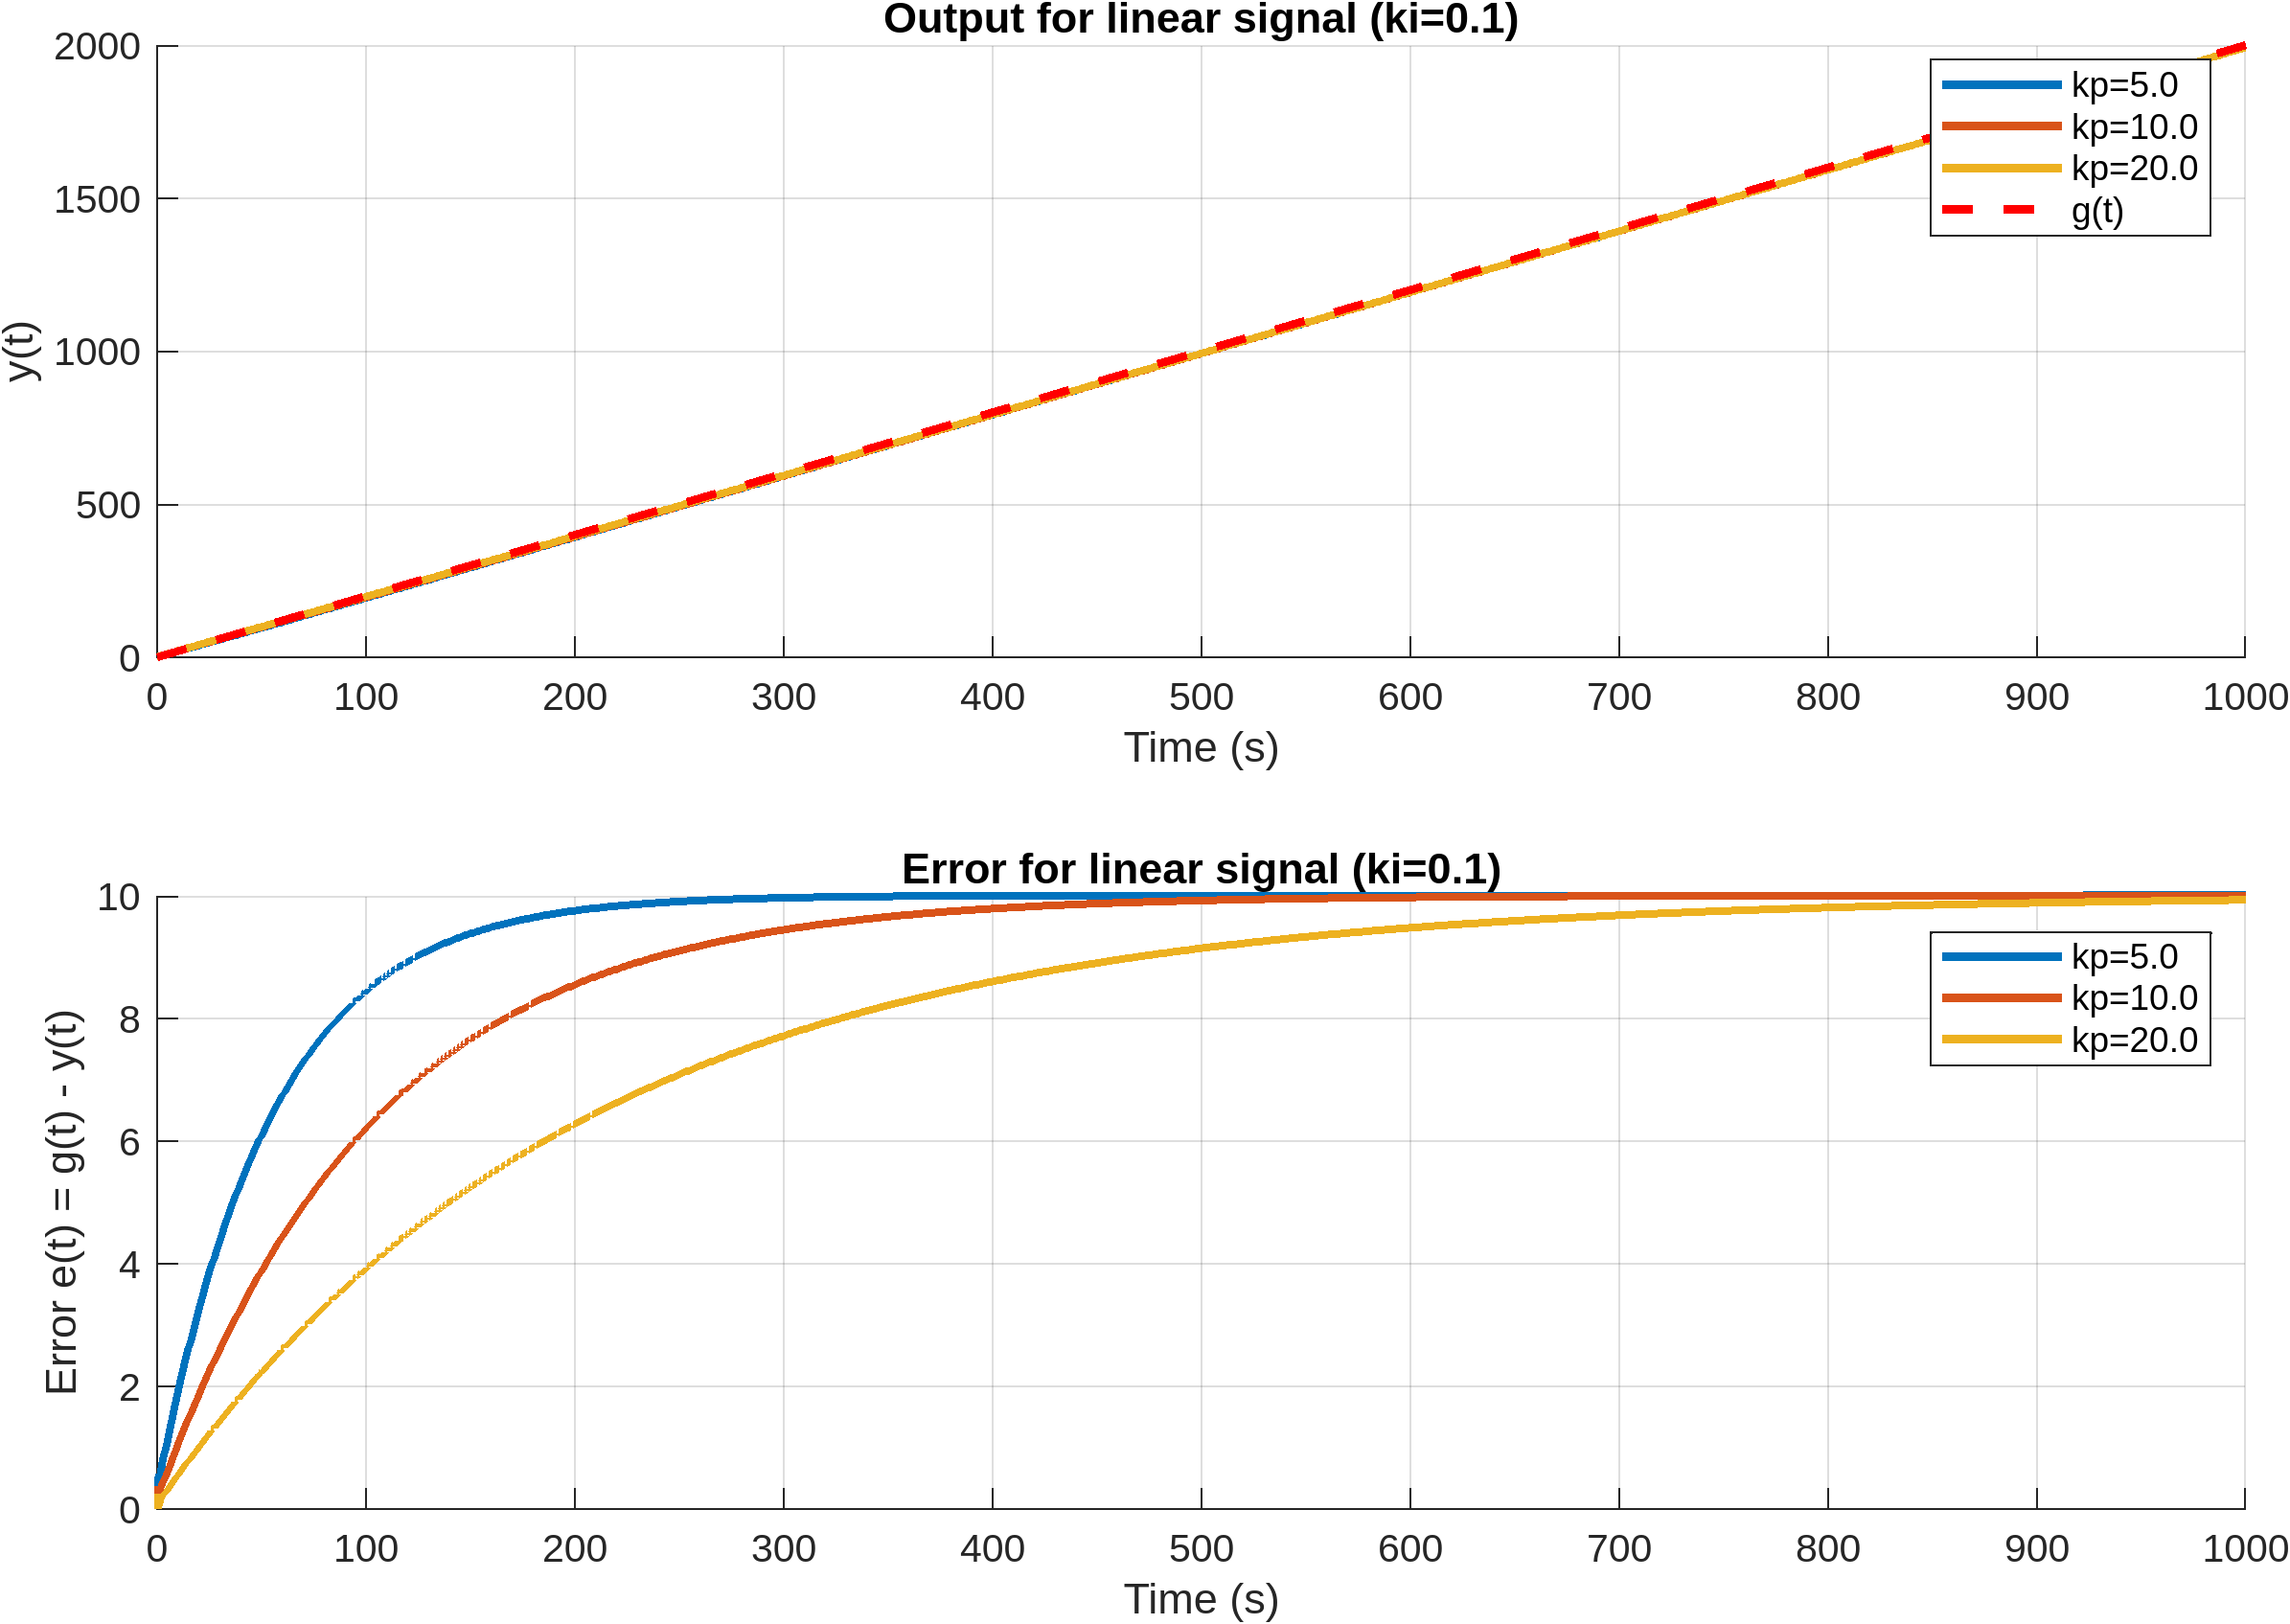
\includegraphics[width=0.85\textwidth]{figs/task_5_out_linear_ki0.1.png}
    \caption{Графики выхода системы с ПИ регулятором при линейном входном сигнале (\( k_i = 0.1 \)).}
    \label{fig:task_5_out_linear_ki0.1}
\end{figure}

\begin{figure}[H]
    \centering
    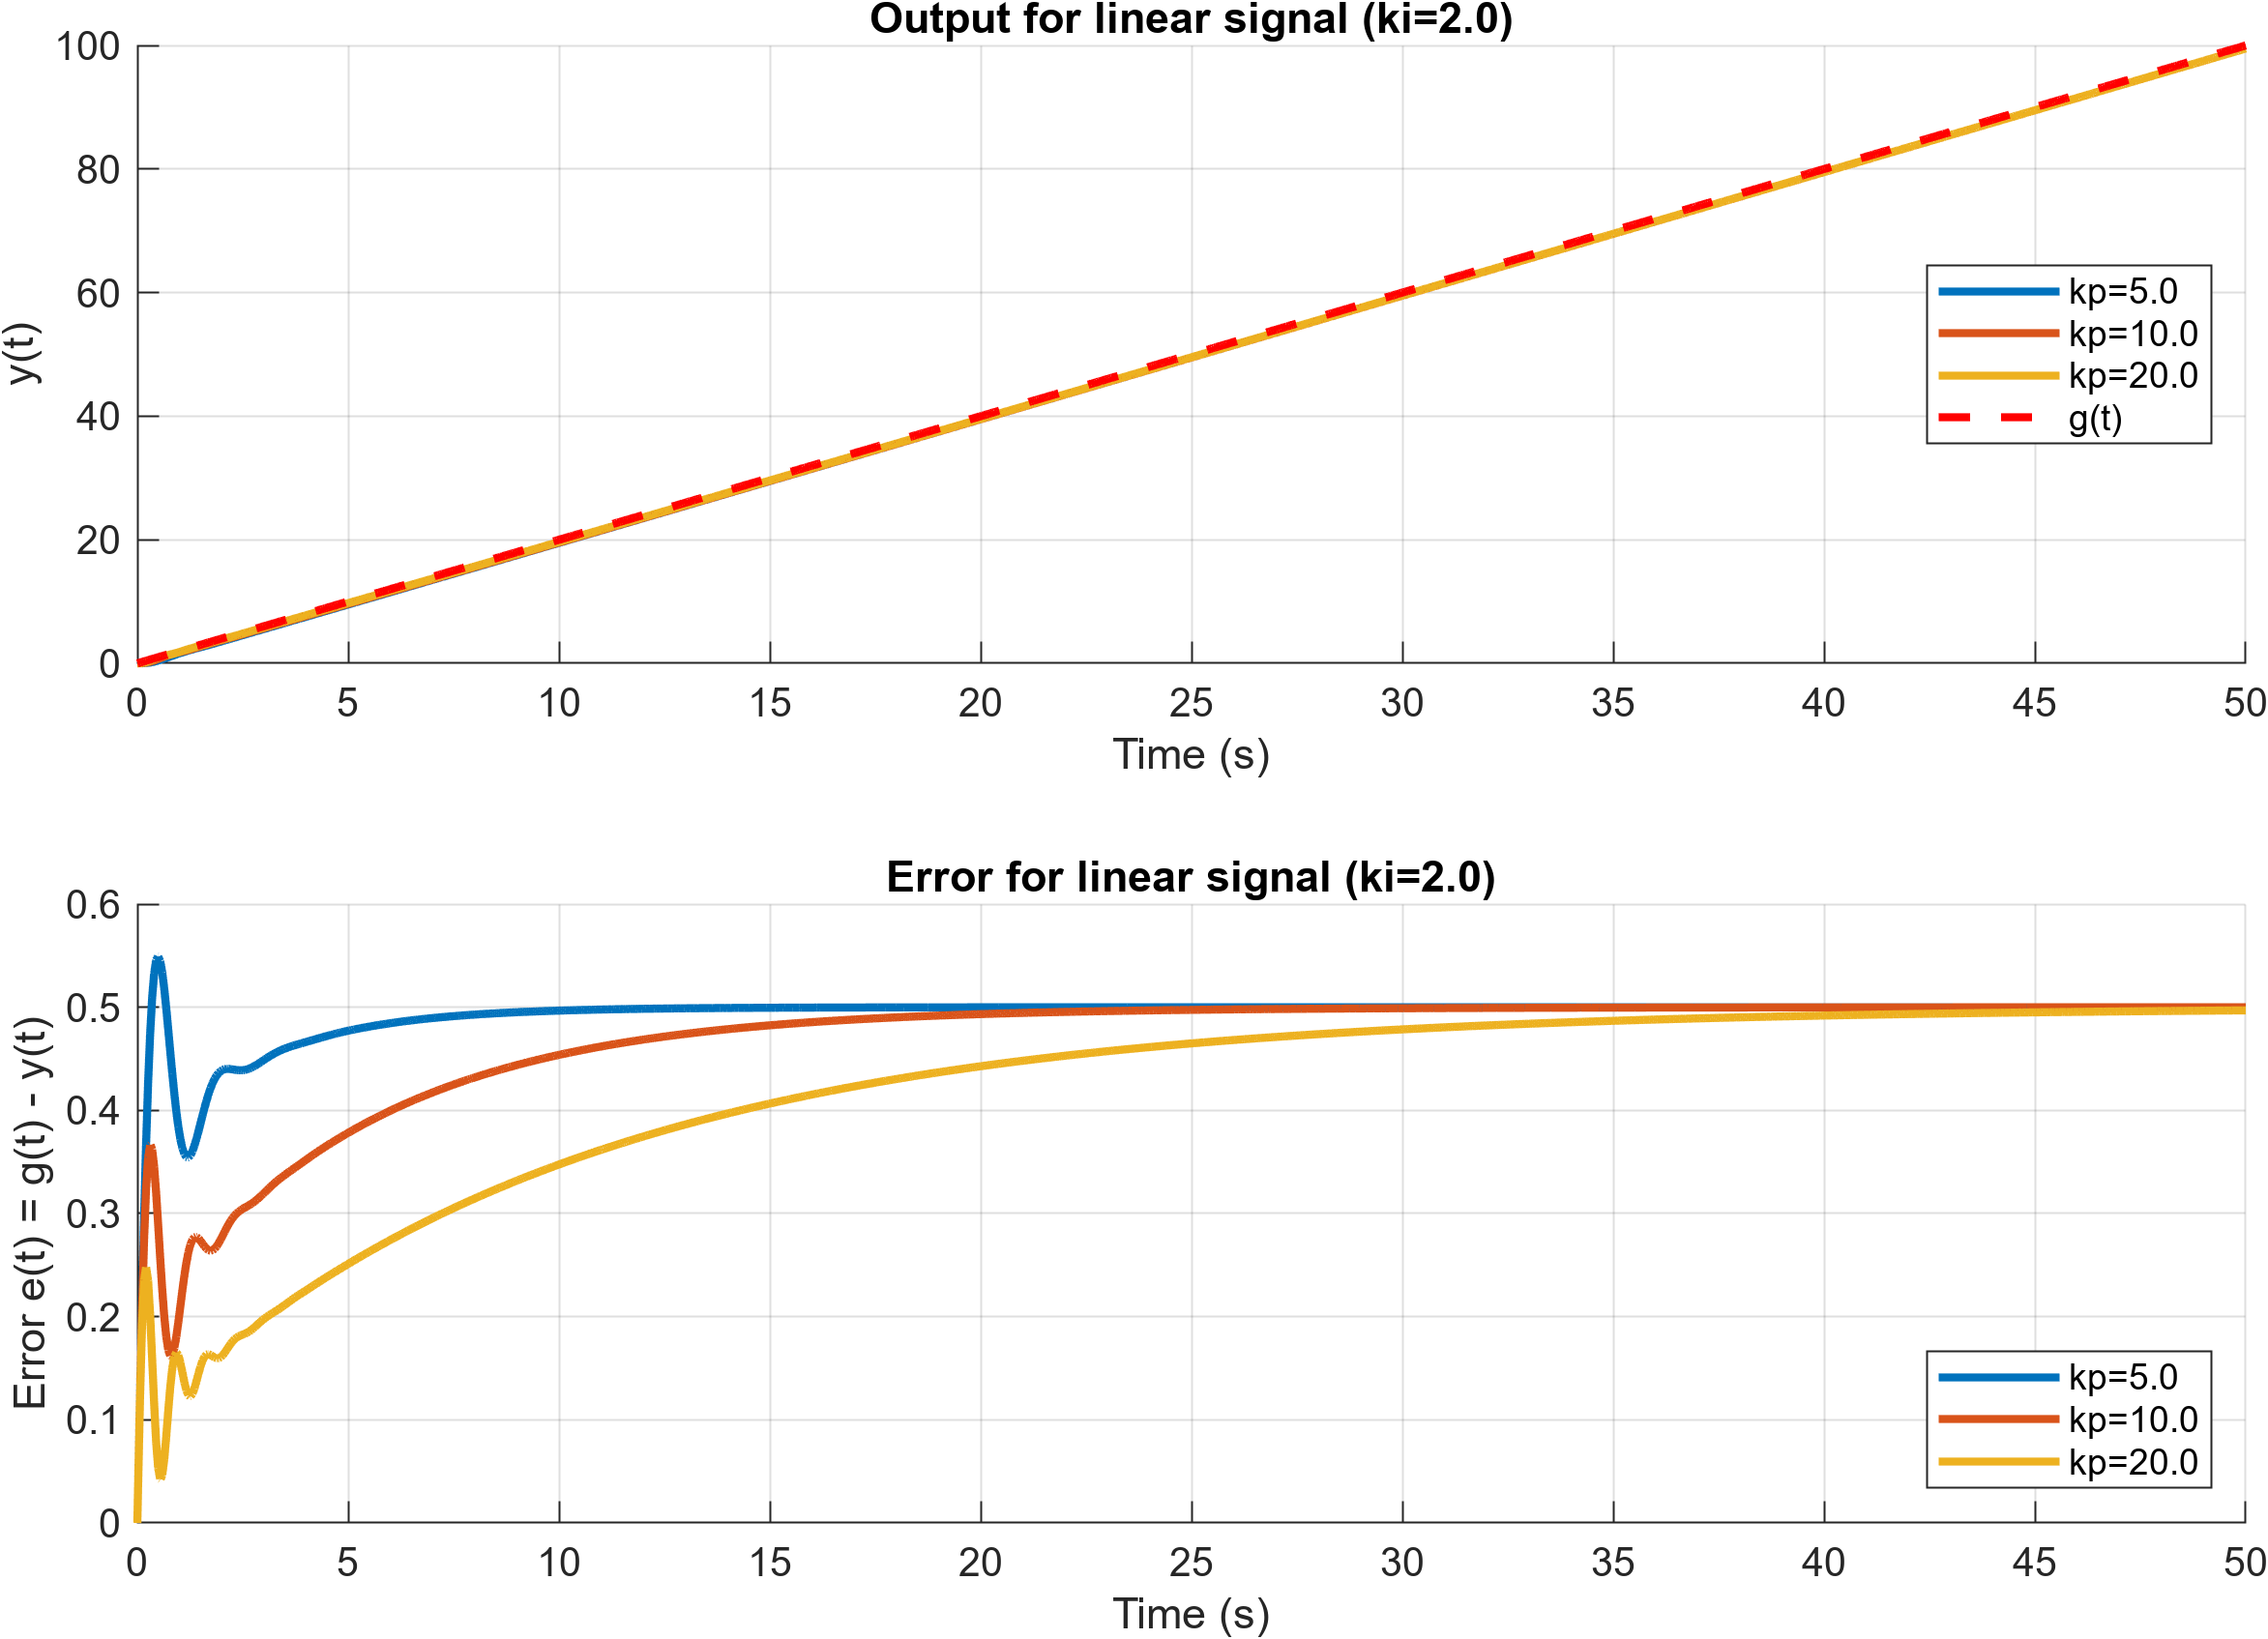
\includegraphics[width=0.85\textwidth]{figs/task_5_out_linear_ki2.0.png}
    \caption{Графики выхода системы с ПИ регулятором при линейном входном сигнале (\( k_i = 2.0 \)).}
    \label{fig:task_5_out_linear_ki2.0}
\end{figure}

\begin{figure}[H]
    \centering
    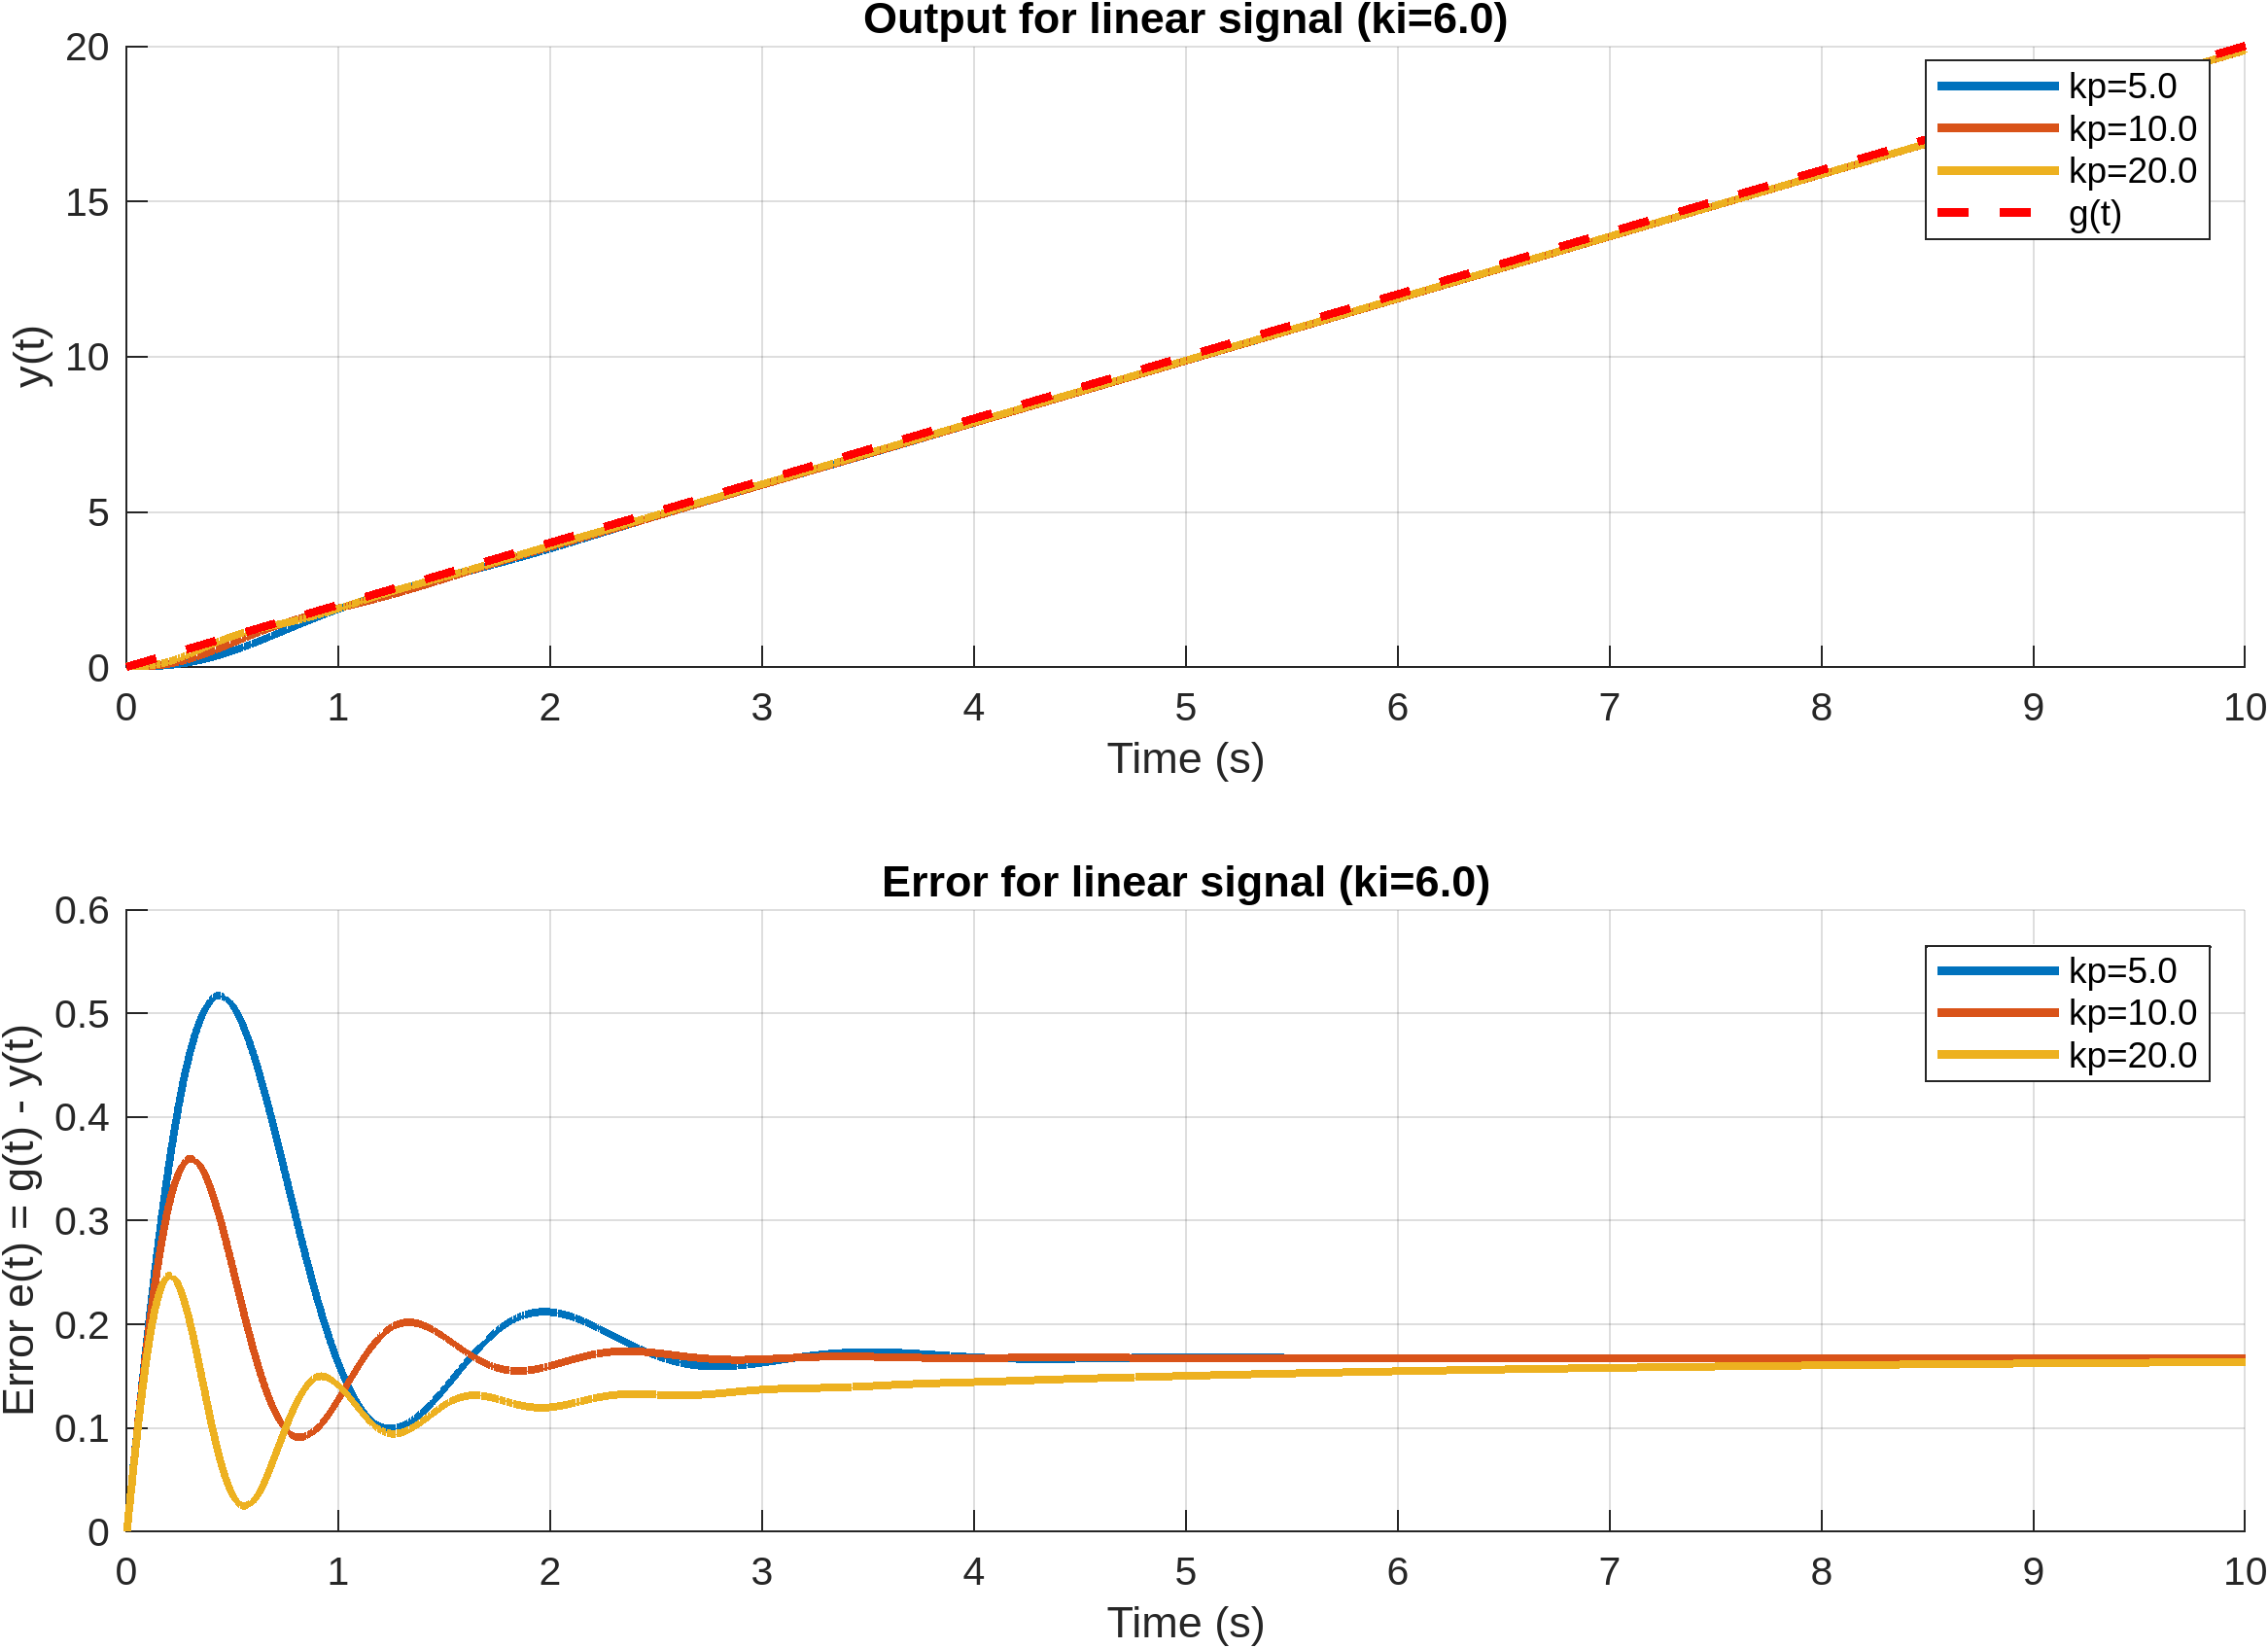
\includegraphics[width=0.85\textwidth]{figs/task_5_out_linear_ki6.0.png}
    \caption{Графики выхода системы с ПИ регулятором при линейном входном сигнале (\( k_i = 6.0 \)).}
    \label{fig:task_5_out_linear_ki6.0}
\end{figure}

% Гармонический сигнал
\begin{figure}[H]
    \centering
    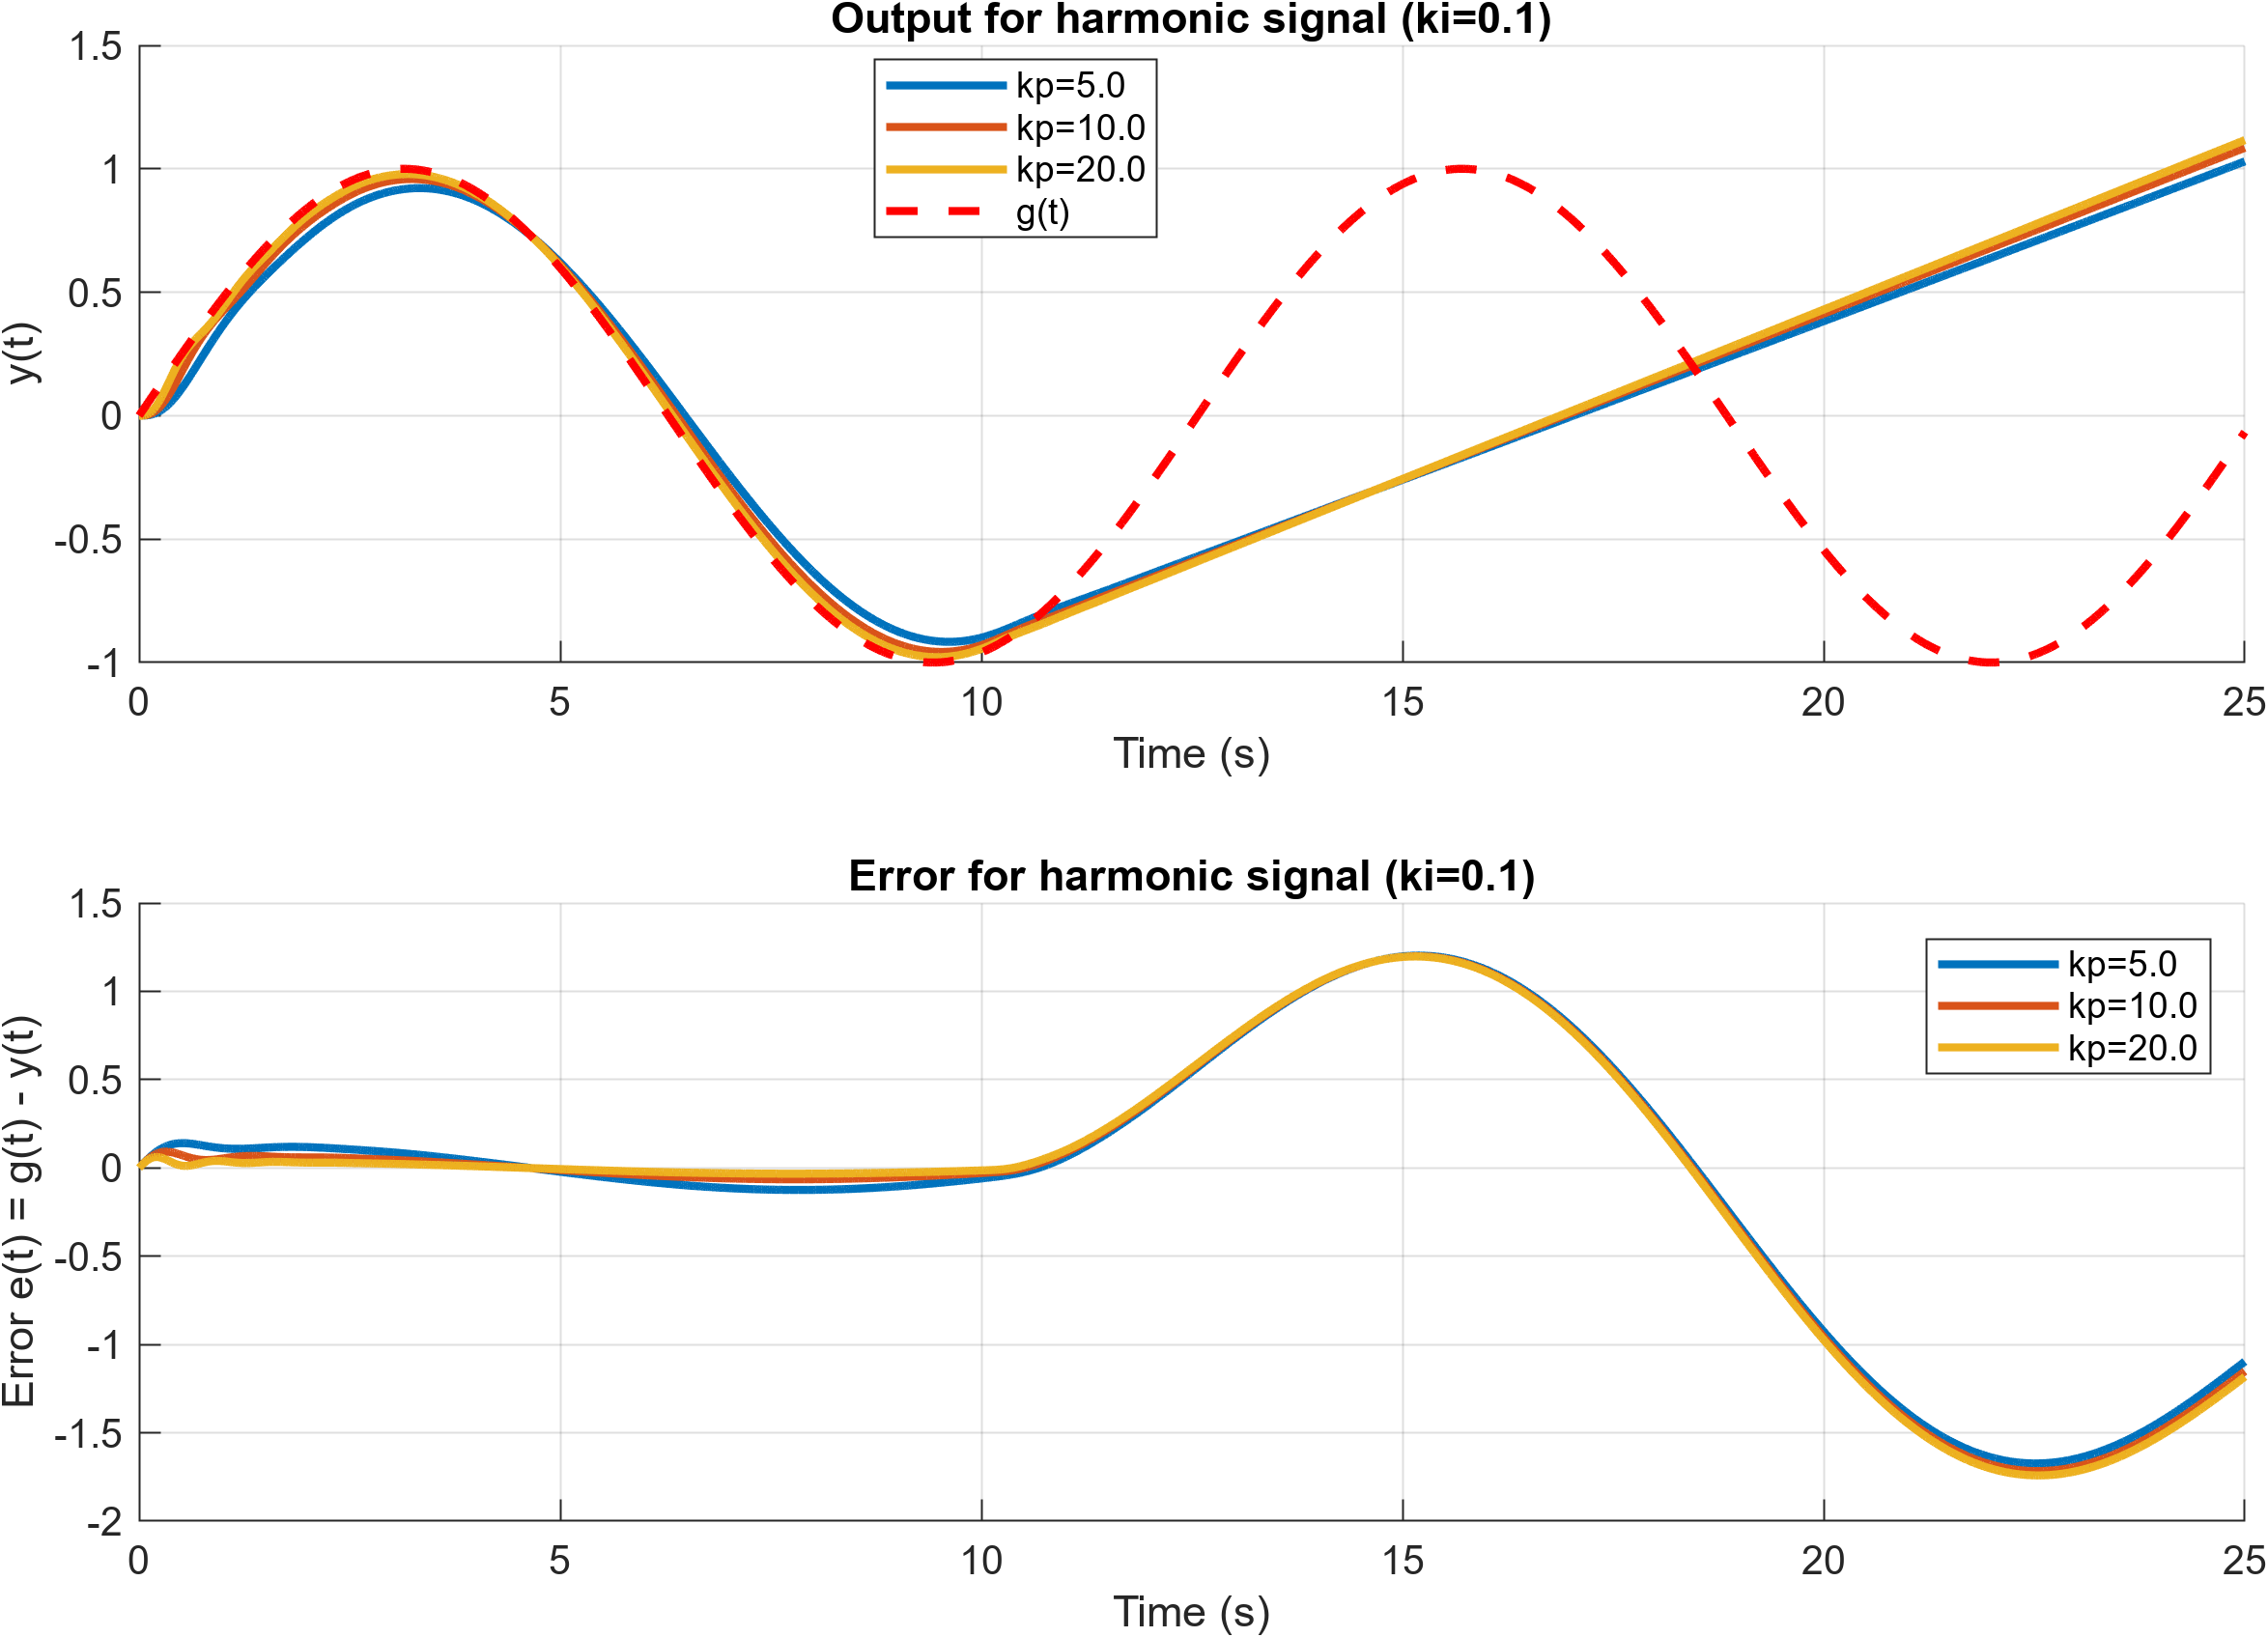
\includegraphics[width=0.85\textwidth]{figs/task_5_out_harmonic_ki0.1.png}
    \caption{Графики выхода системы с ПИ регулятором при гармоническом входном сигнале (\( k_i = 0.1 \)).}
    \label{fig:task_5_out_harmonic_ki0.1}
\end{figure}

\begin{figure}[H]
    \centering
    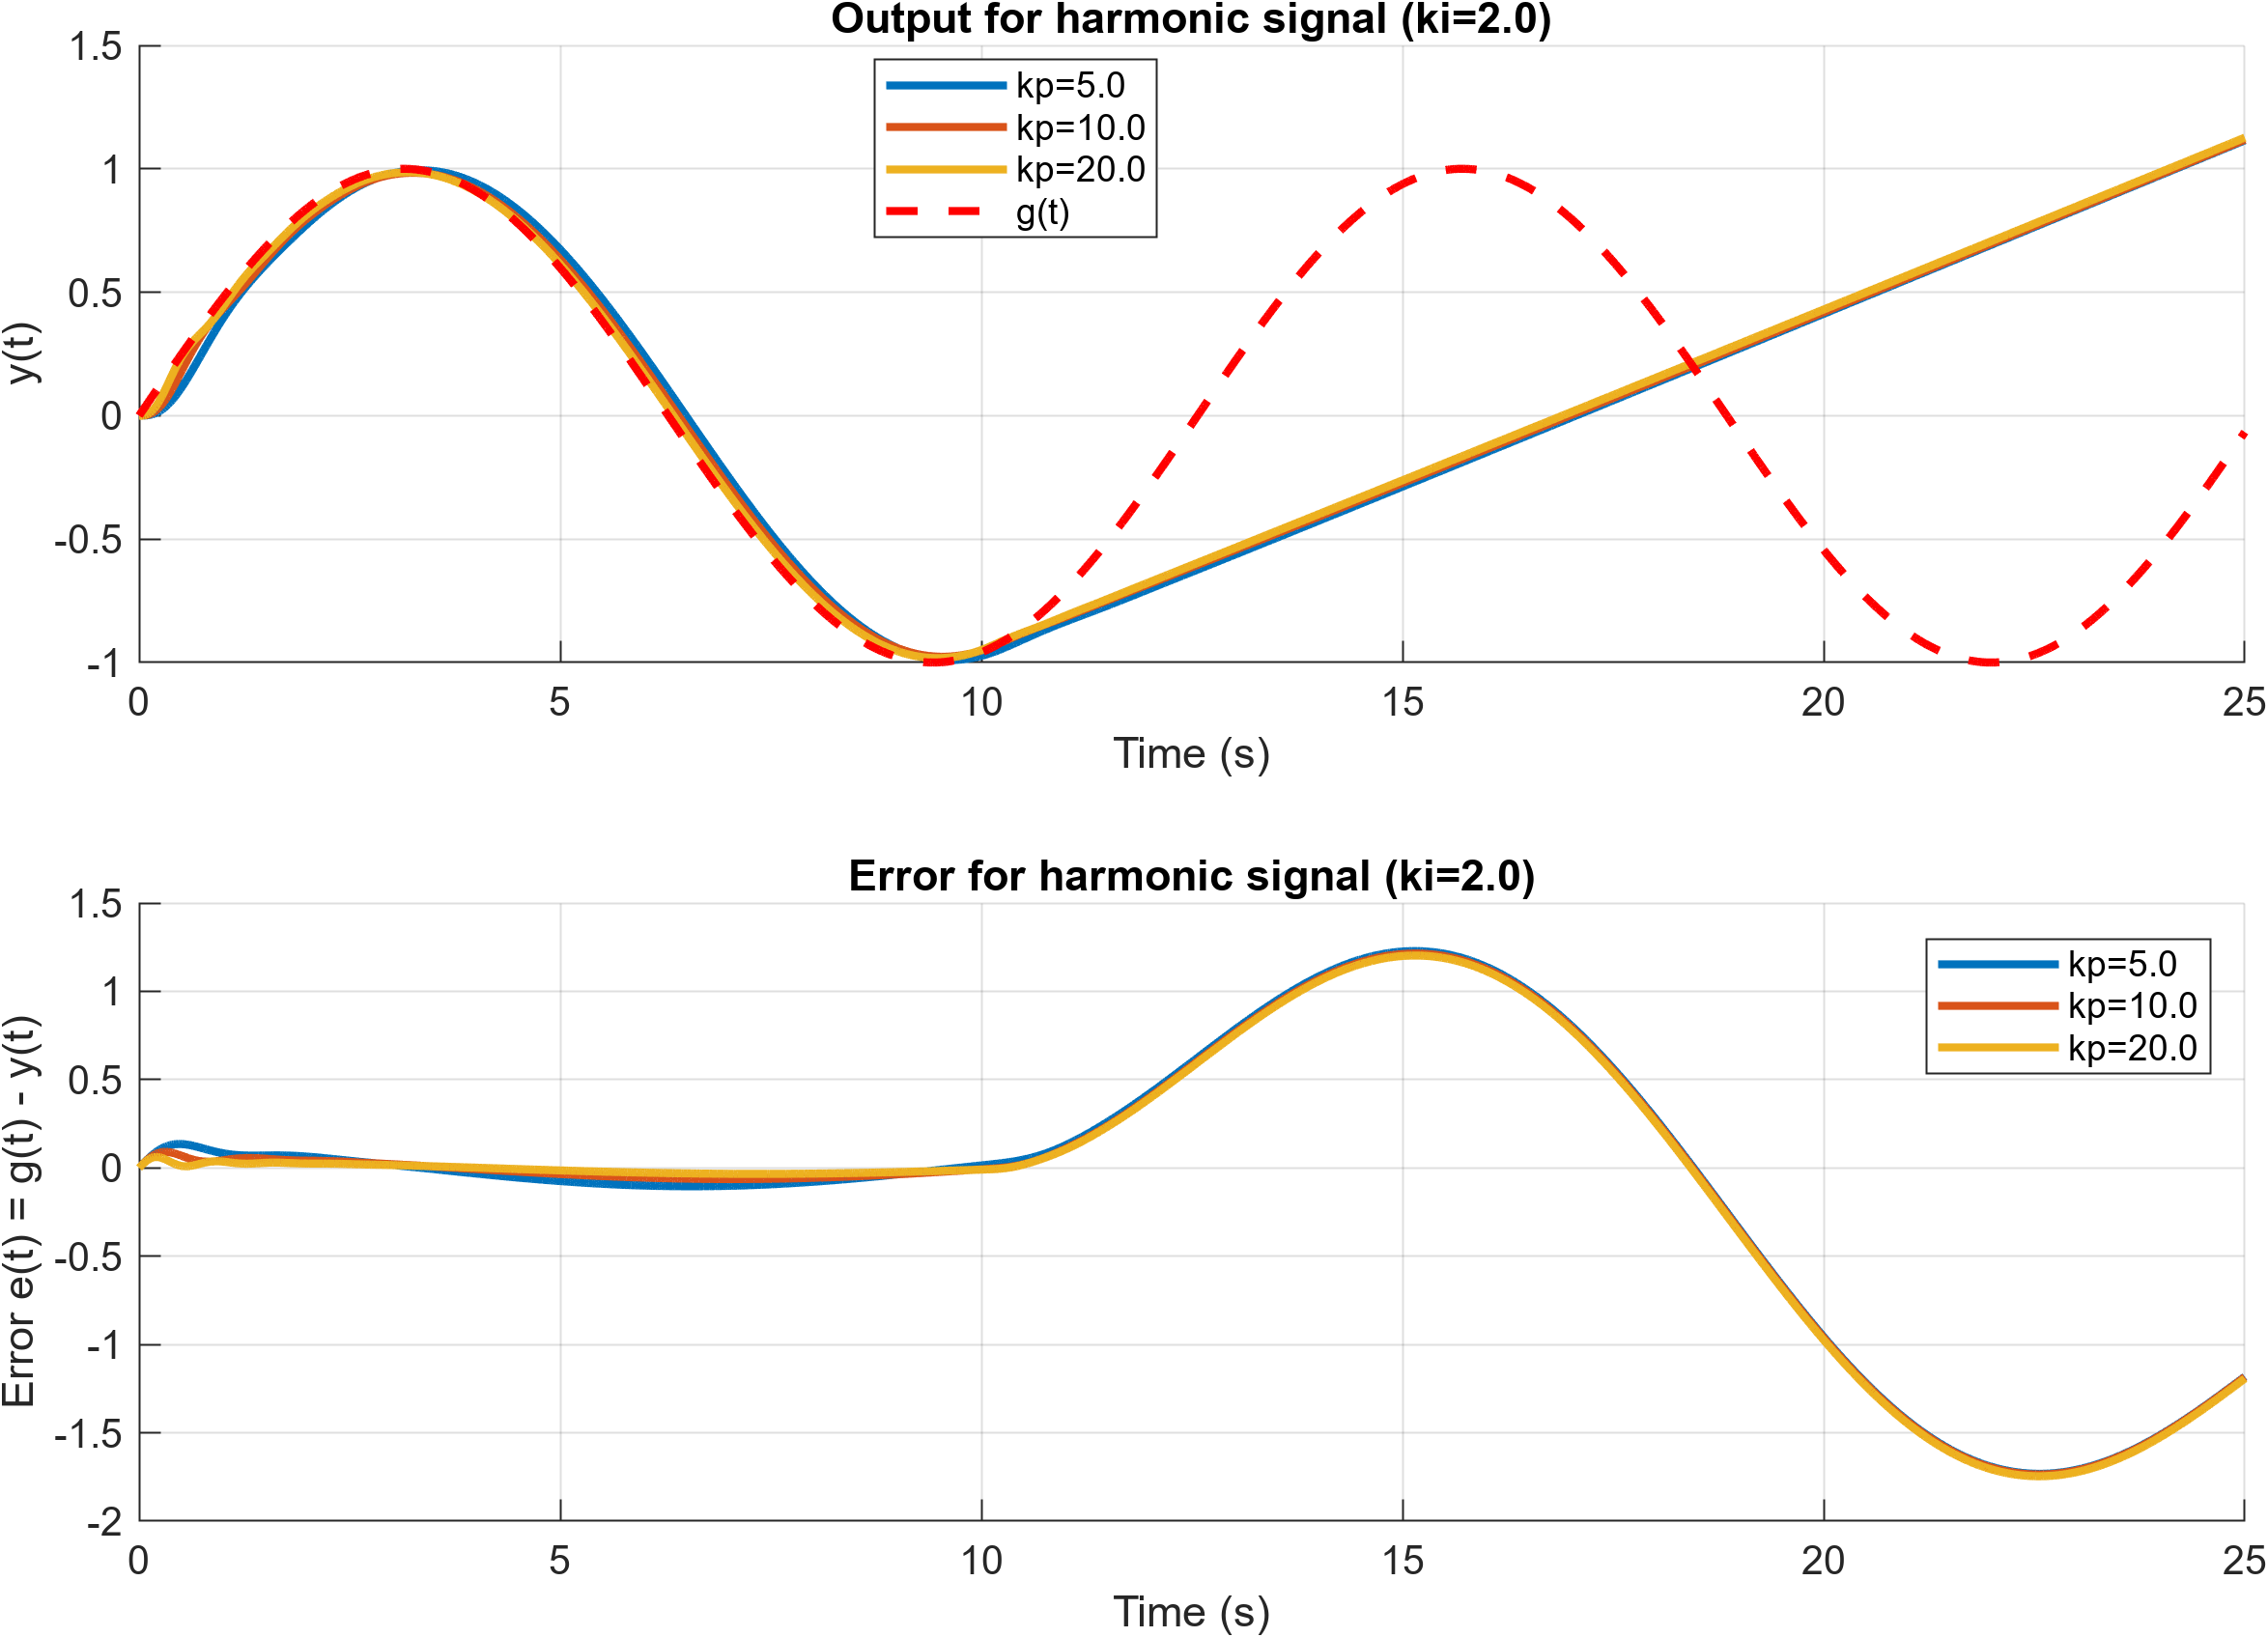
\includegraphics[width=0.85\textwidth]{figs/task_5_out_harmonic_ki2.0.png}
    \caption{Графики выхода системы с ПИ регулятором при гармоническом входном сигнале (\( k_i = 2.0 \)).}
    \label{fig:task_5_out_harmonic_ki2.0}
\end{figure}

\begin{figure}[H]
    \centering
    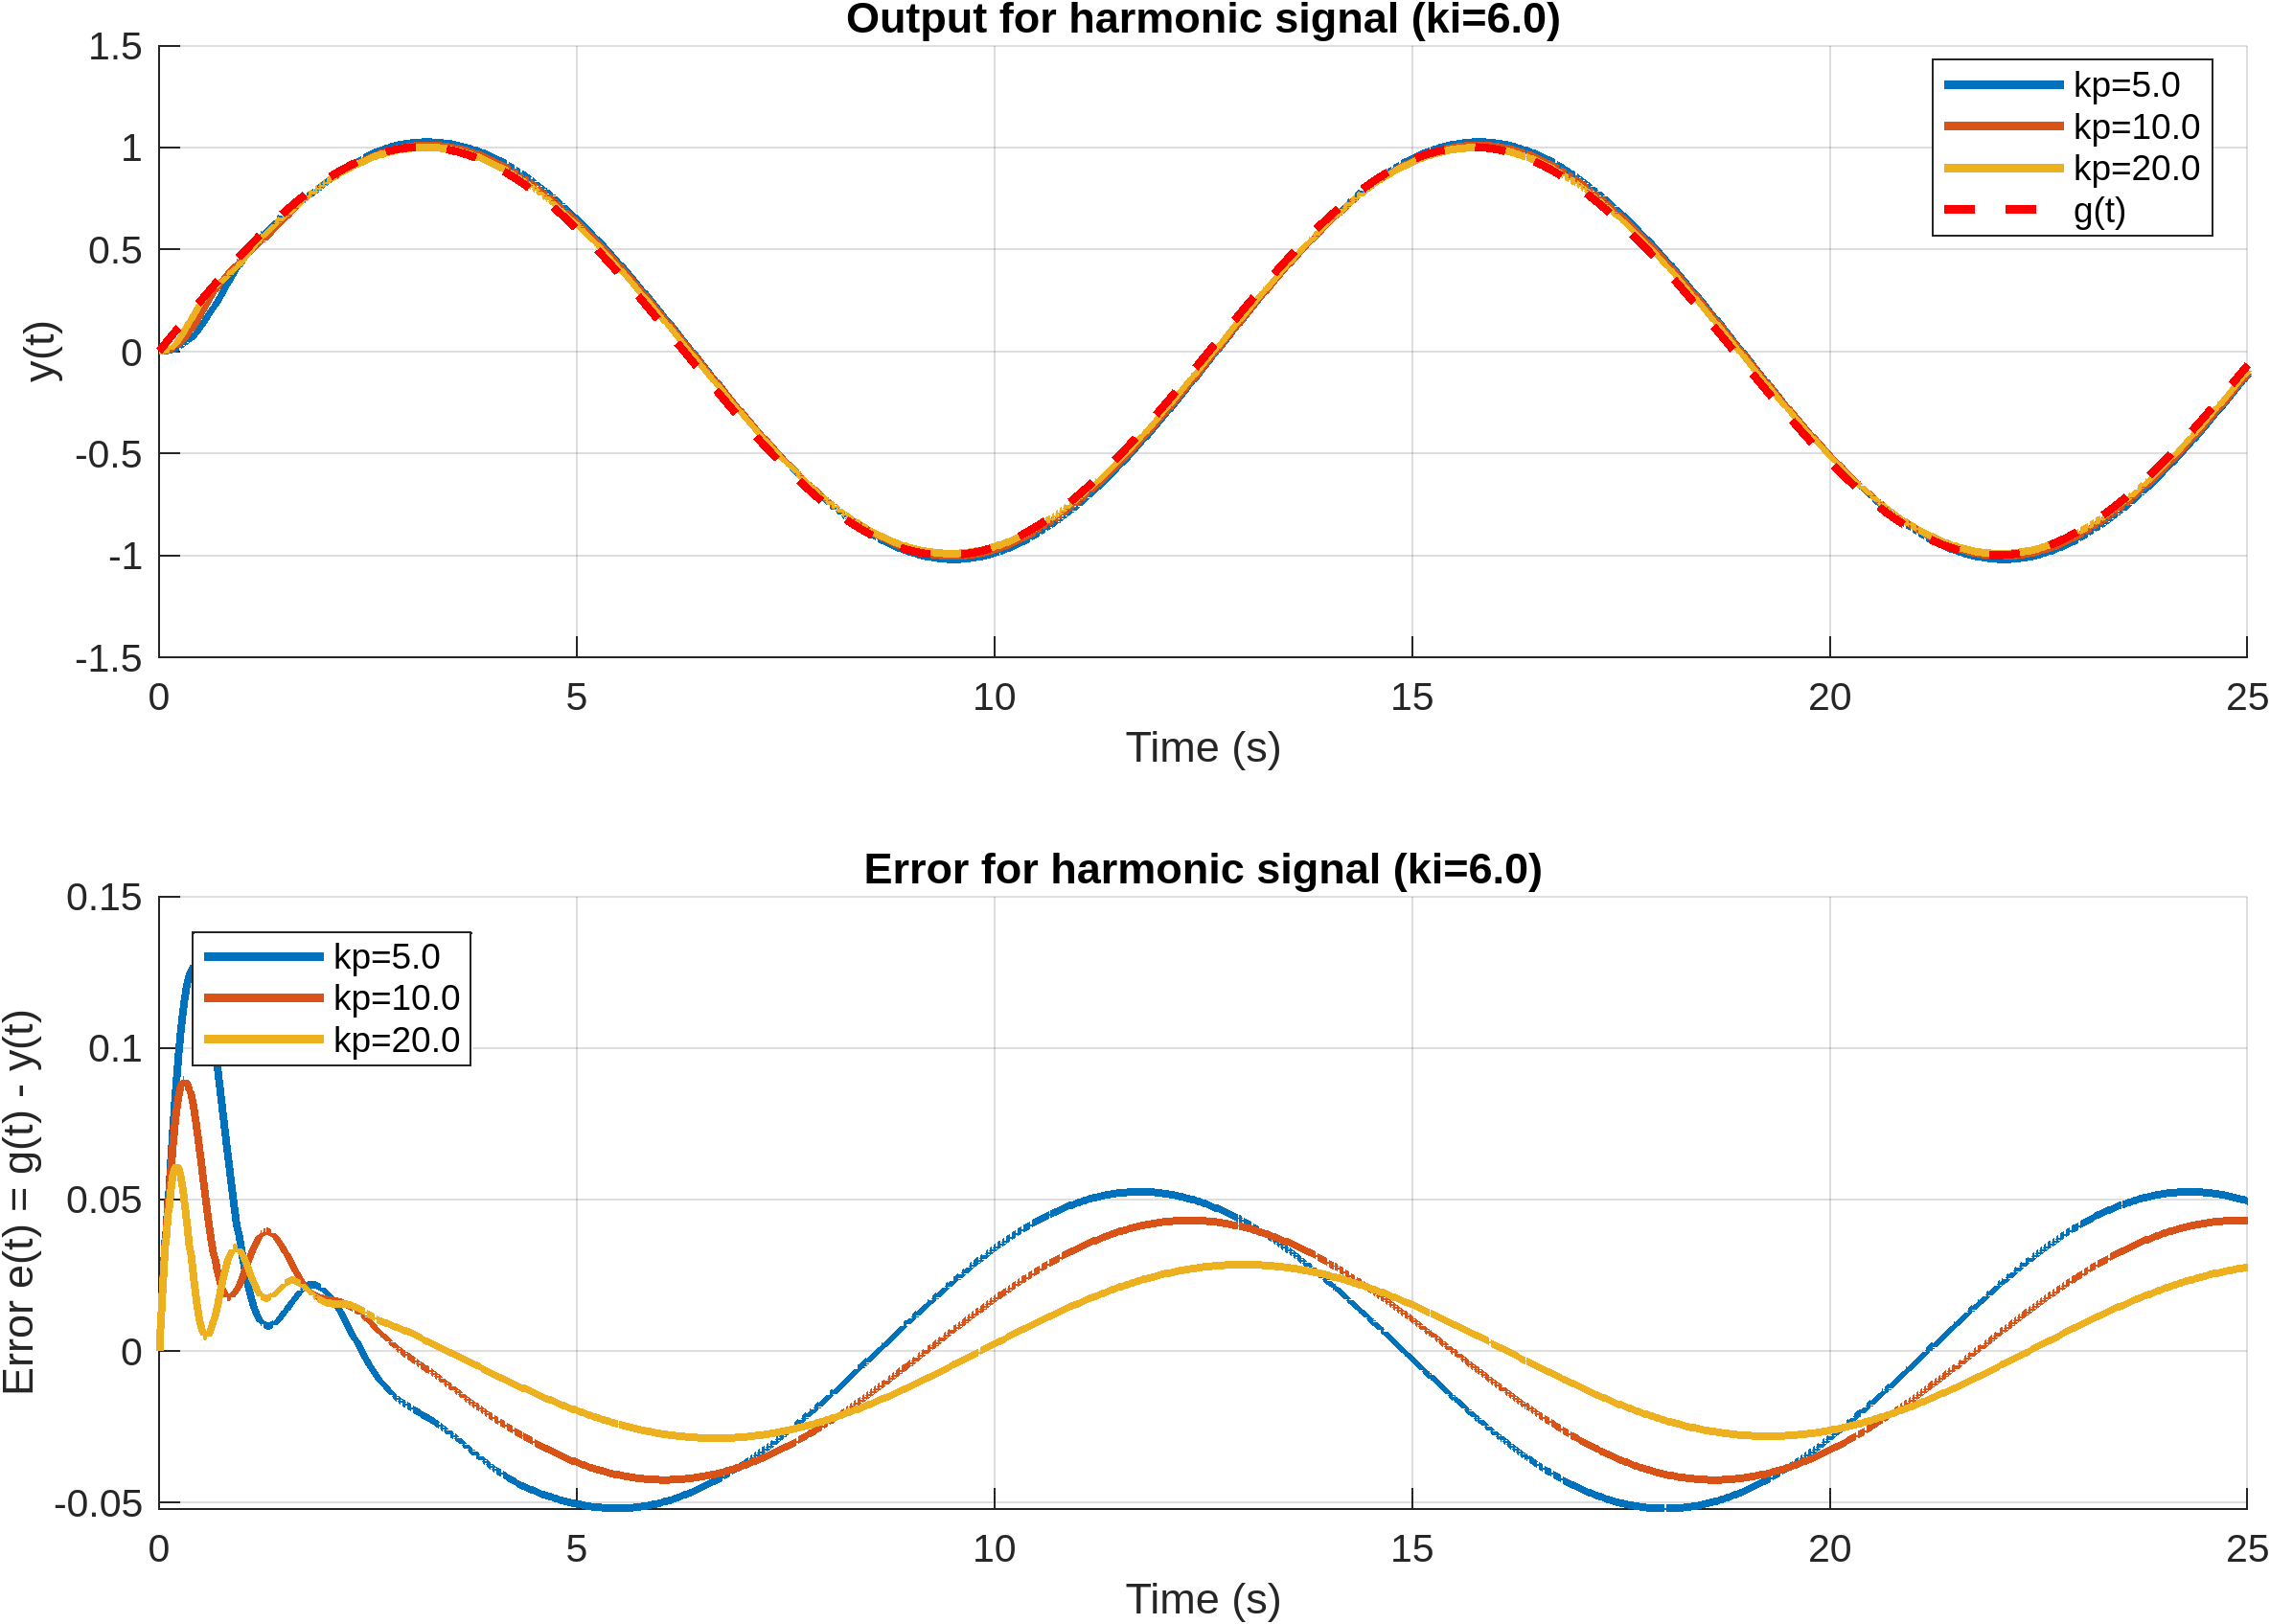
\includegraphics[width=0.85\textwidth]{figs/task_5_out_harmonic_ki6.0.png}
    \caption{Графики выхода системы с ПИ регулятором при гармоническом входном сигнале (\( k_i = 6.0 \)).}
    \label{fig:task_5_out_harmonic_ki6.0}
\end{figure}

% Линейный маленький t
\begin{figure}[H]
    \centering
    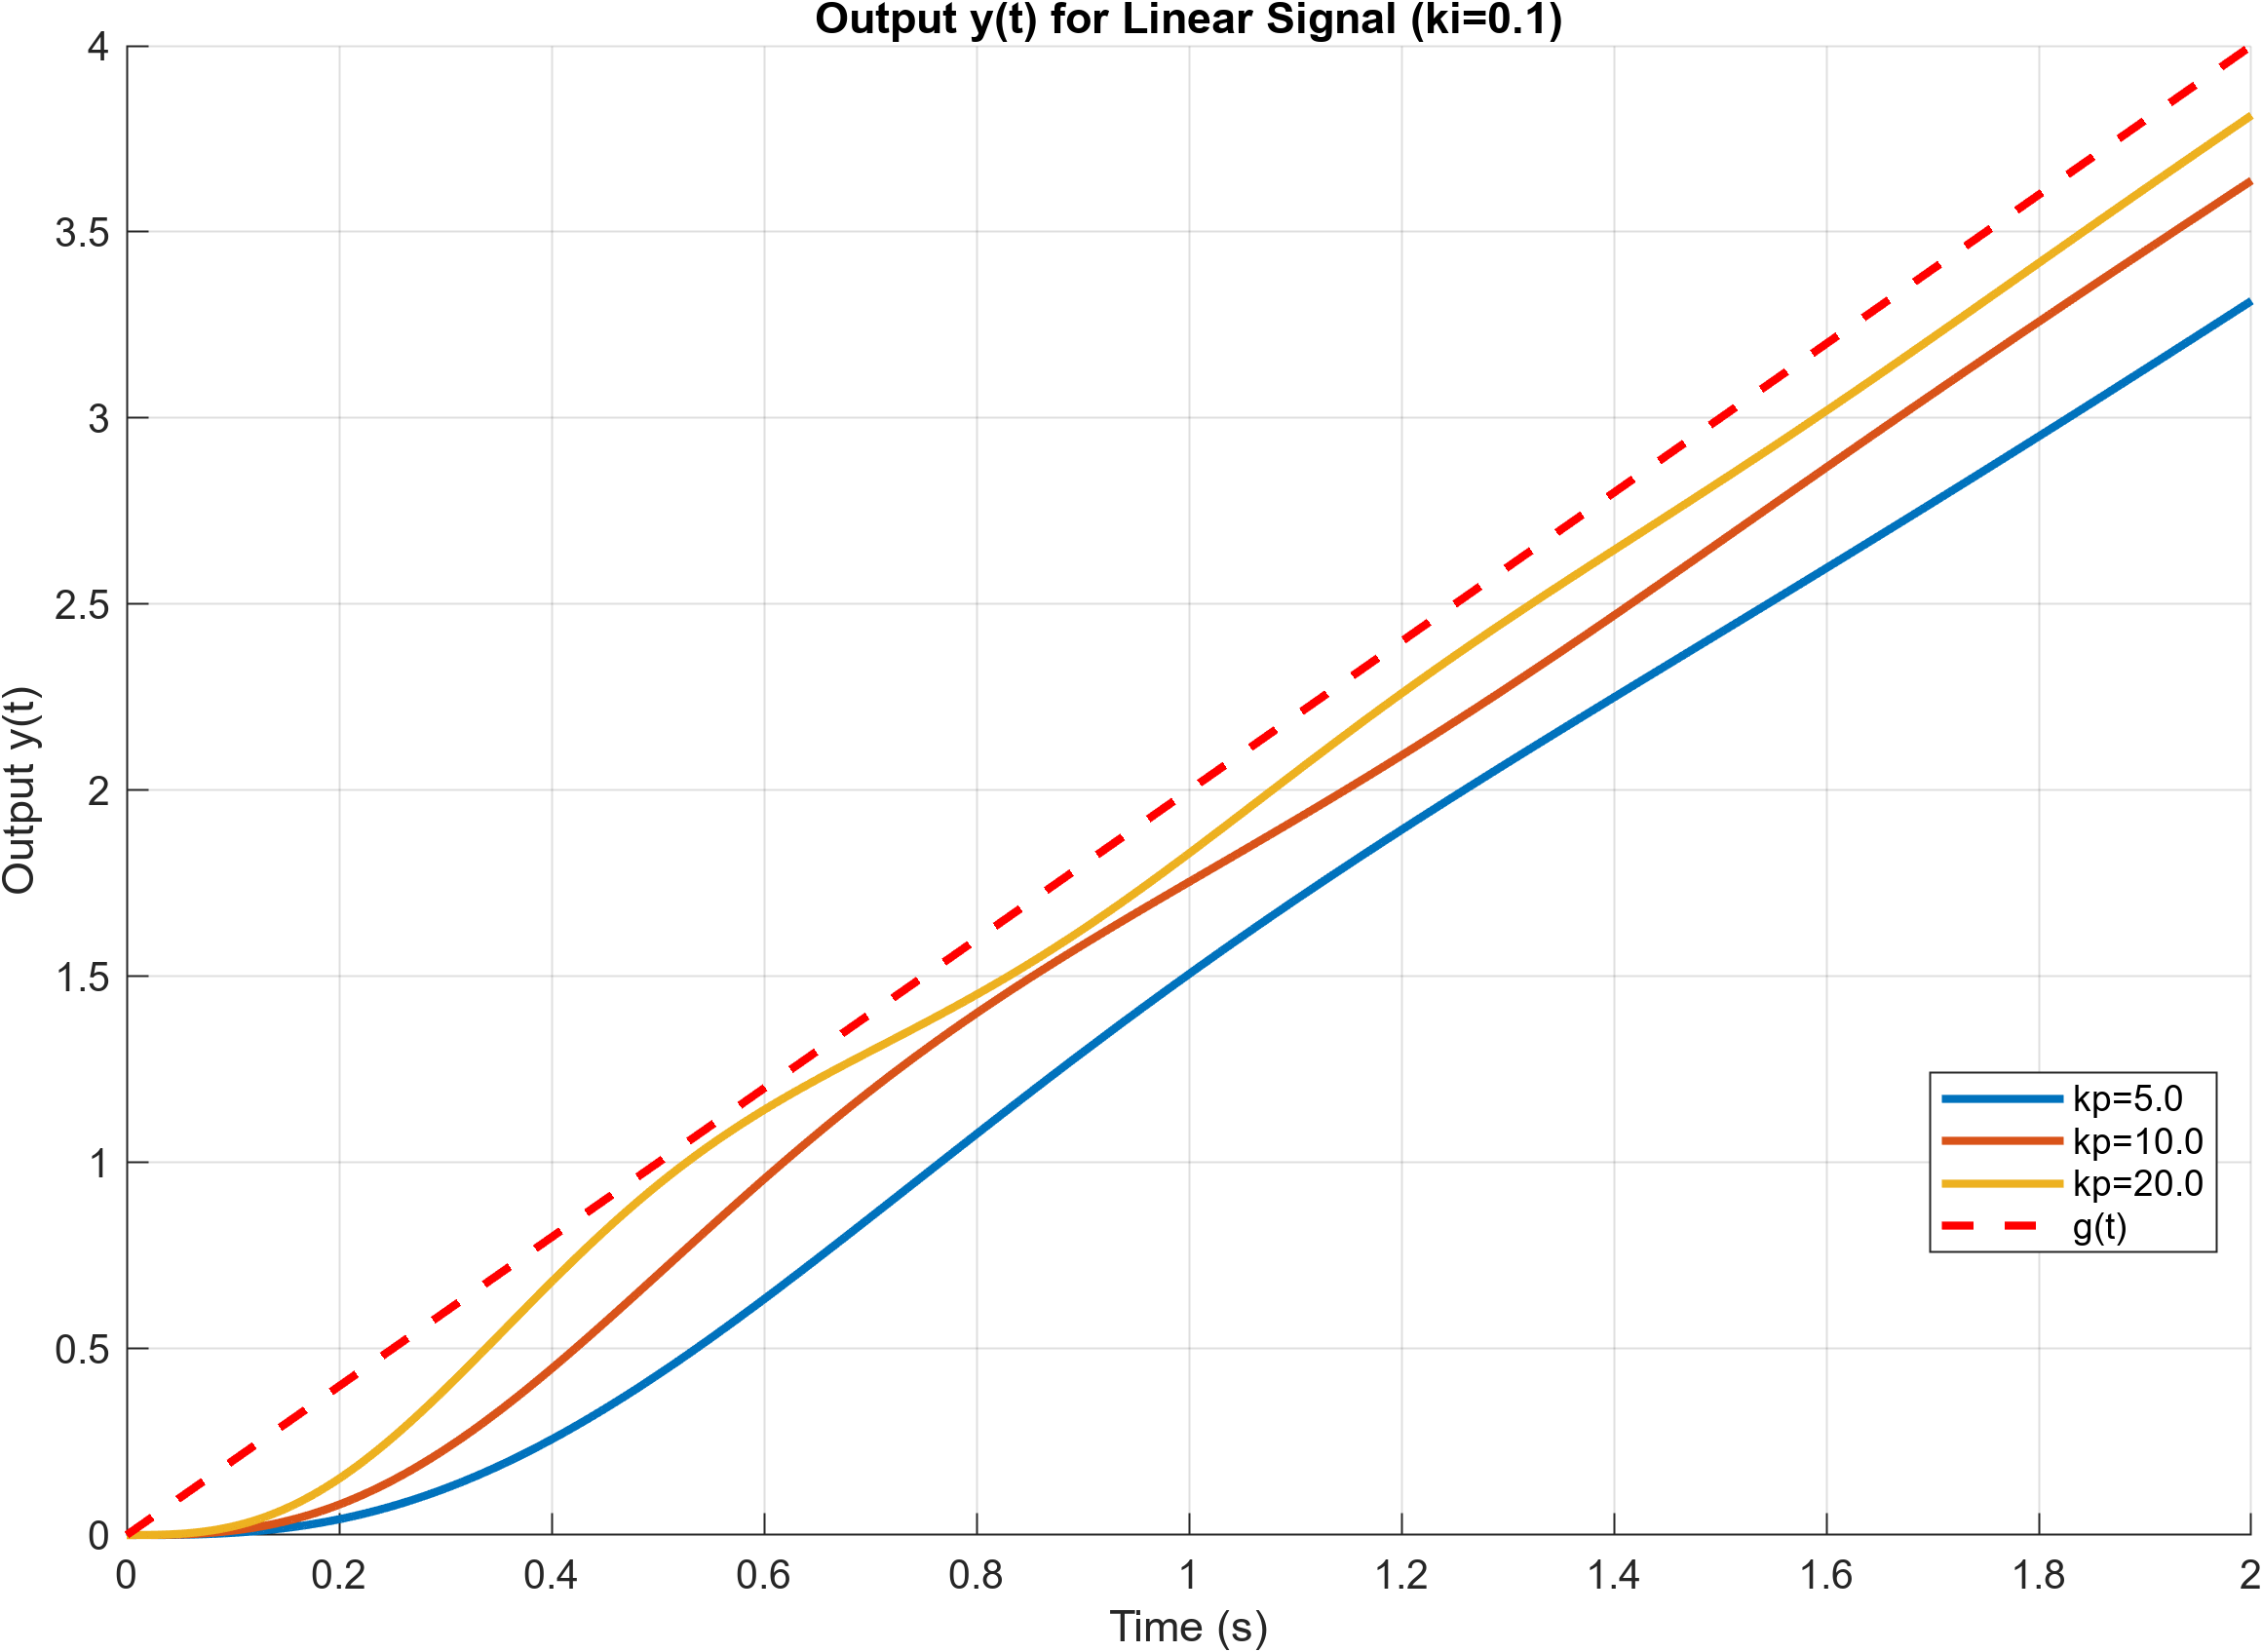
\includegraphics[width=0.85\textwidth]{figs/task_5_output_linear_small_t_ki_0.1.png}
    \caption{Графики выхода системы с ПИ регулятором при линейном входном сигнале (\( k_i = 0.1 \)) на малых $t$.}
    \label{fig:task_5_output_ki_0.1}
\end{figure}

\begin{figure}[H]
    \centering
    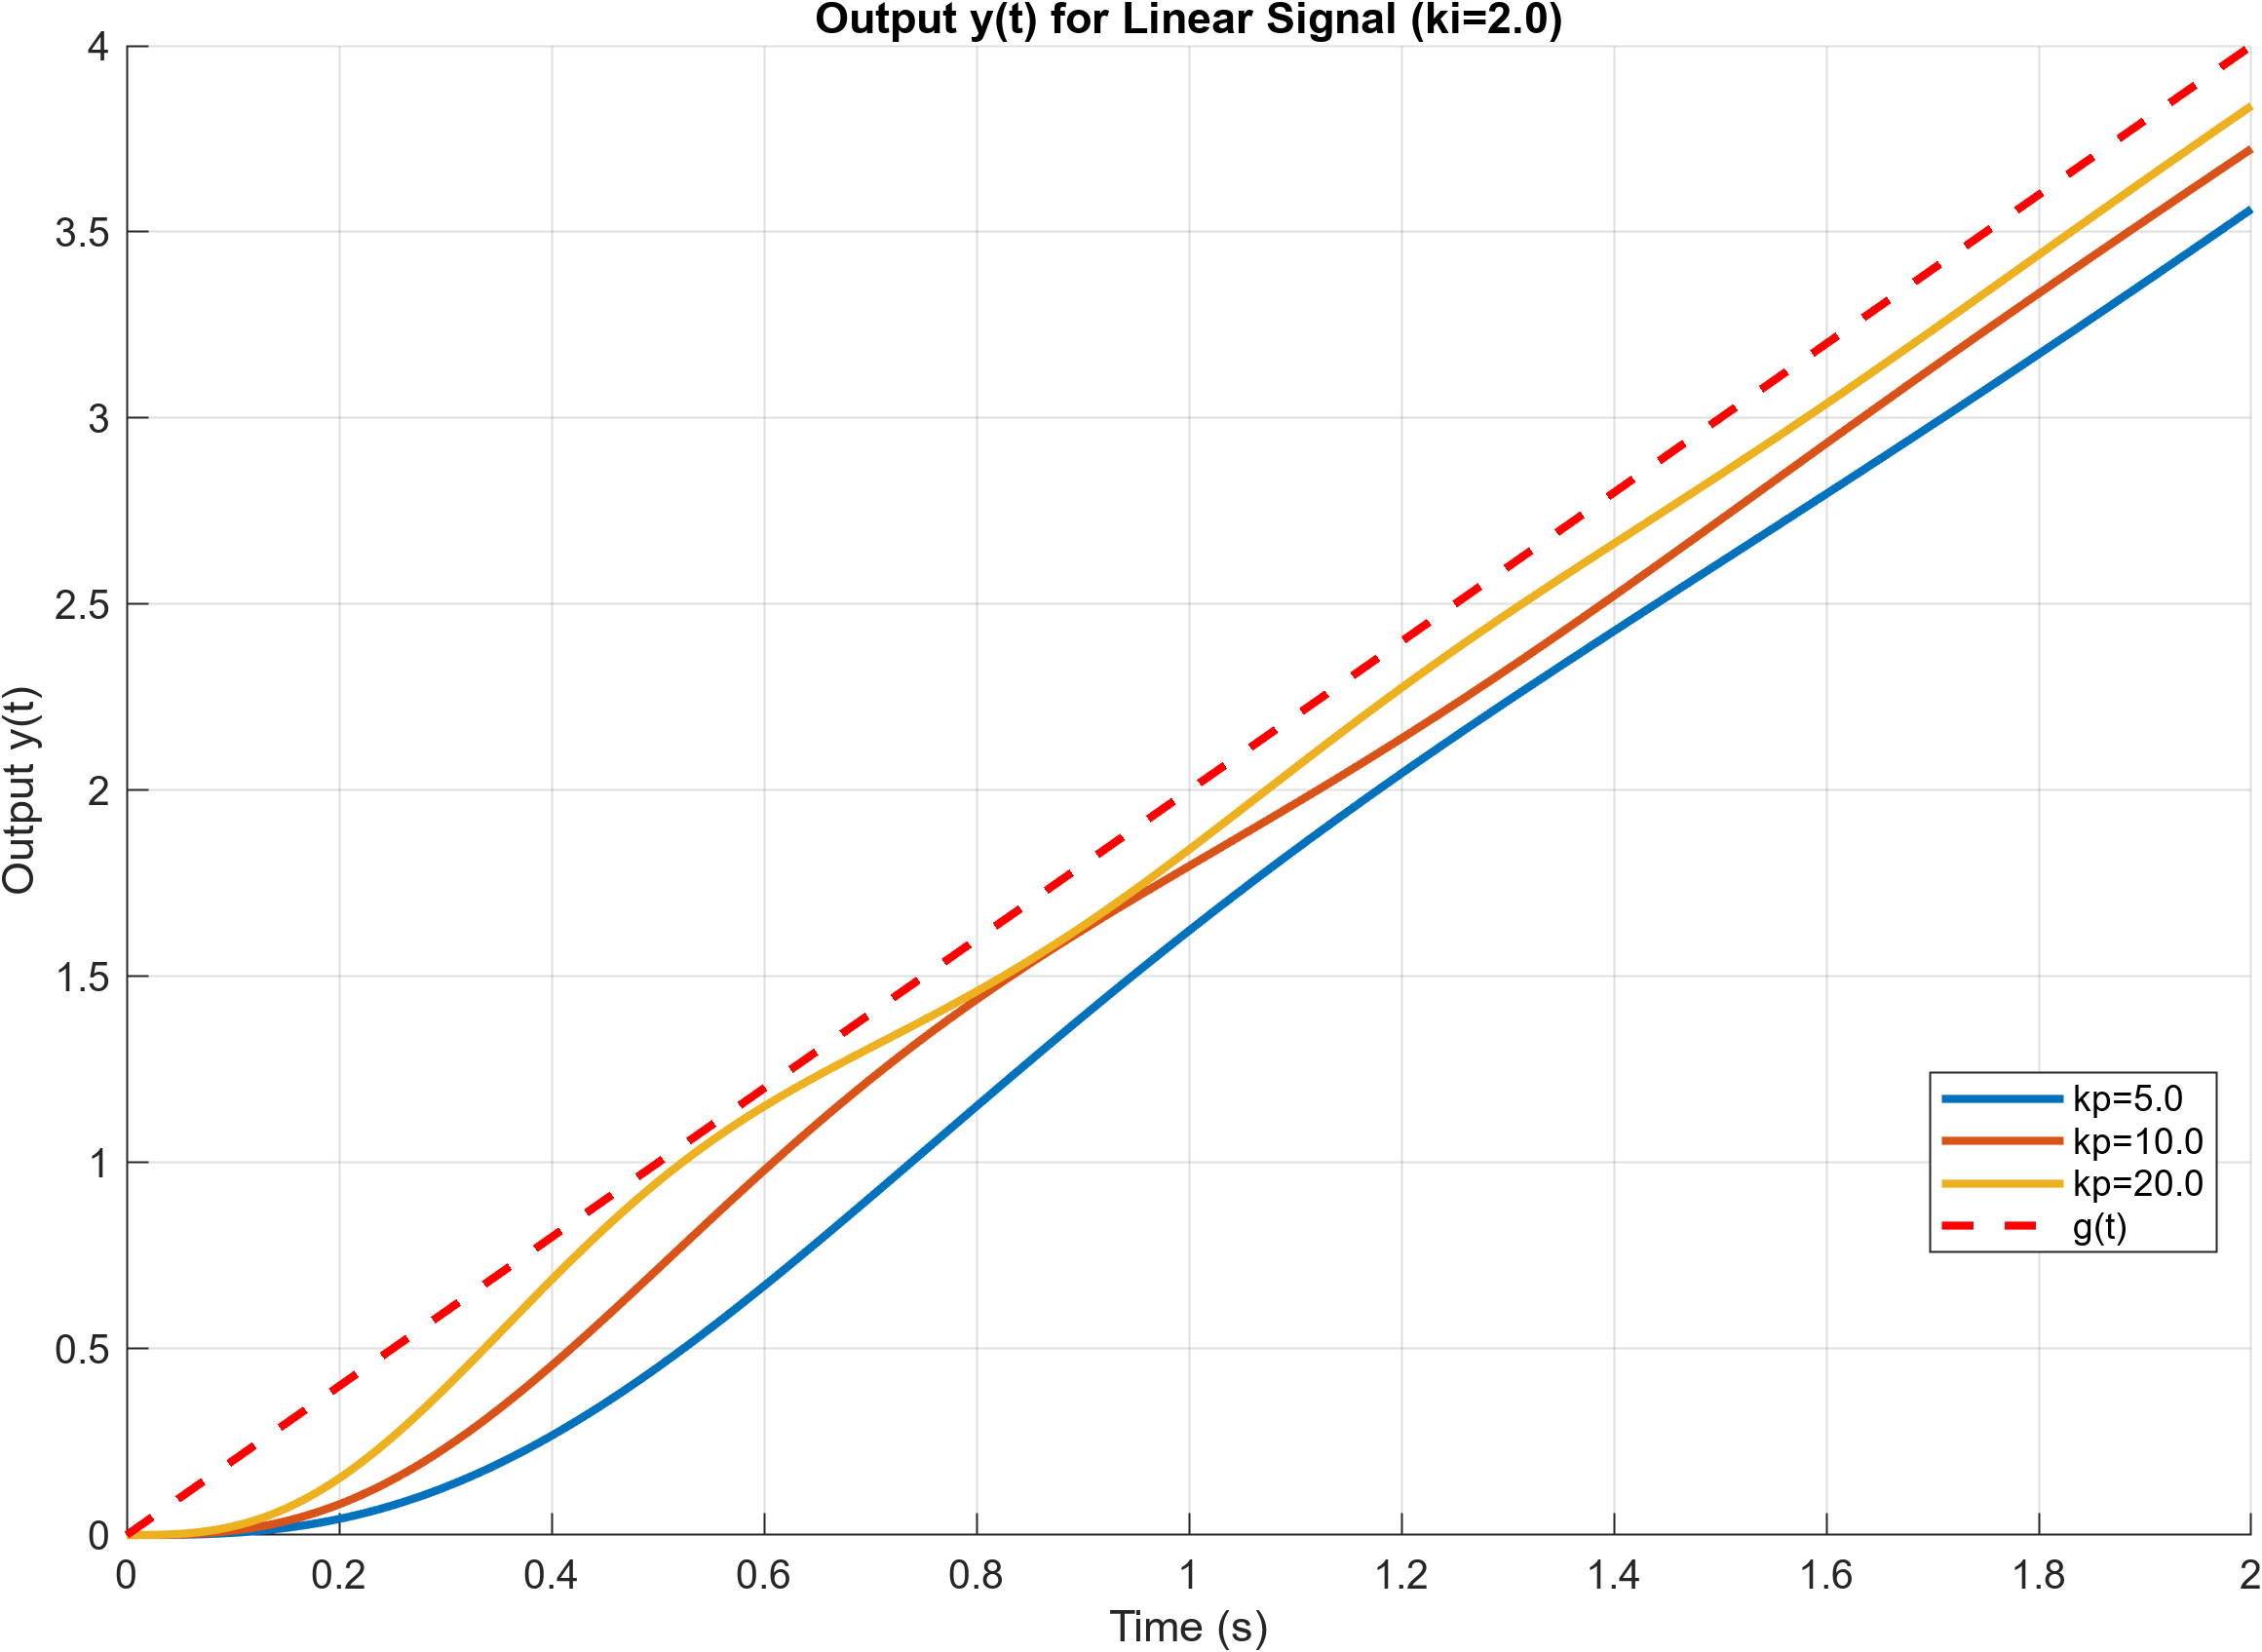
\includegraphics[width=0.85\textwidth]{figs/task_5_output_linear_small_t_ki_2.0.png}
    \caption{Графики выхода системы с ПИ регулятором при линейном входном сигнале (\( k_i = 2.0 \)) на малых $t$.}
    \label{fig:task_5_output_ki_2.0}
\end{figure}

\begin{figure}[H]
    \centering
    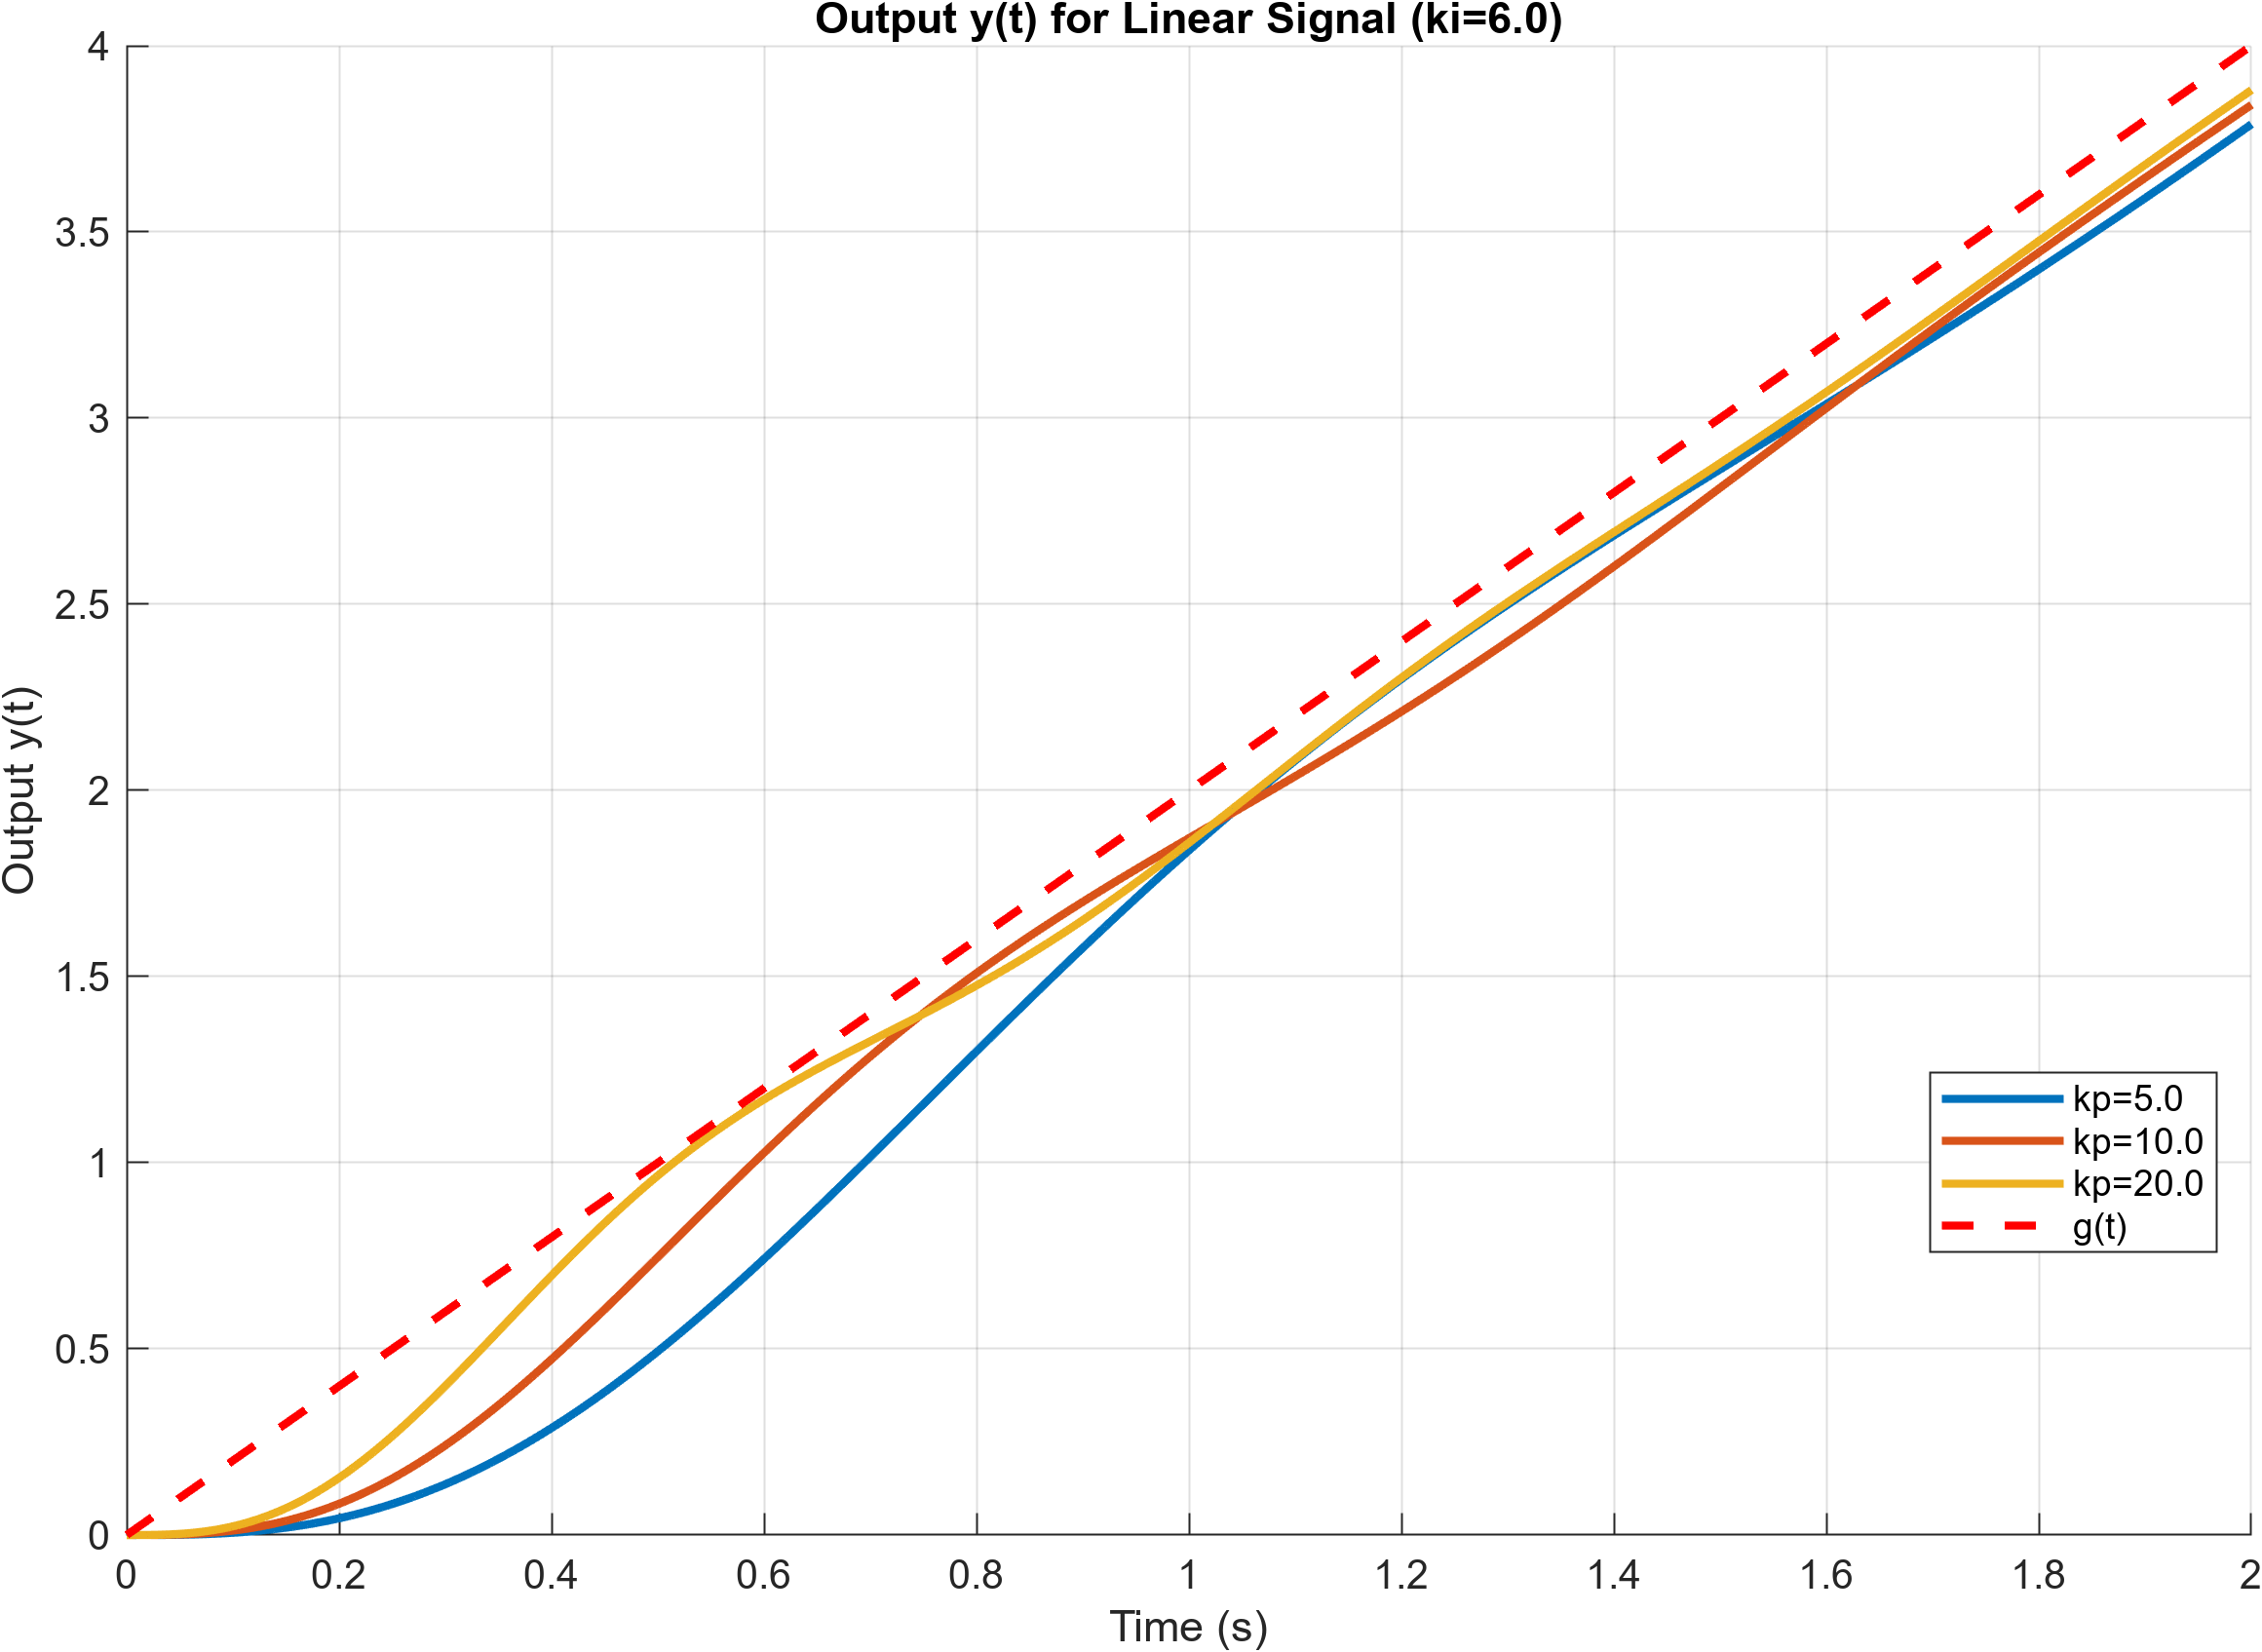
\includegraphics[width=0.85\textwidth]{figs/task_5_output_linear_small_t_ki_6.0.png}
    \caption{Графики выхода системы с ПИ регулятором при линейном входном сигнале (\( k_i = 6.0 \)) на малых $t$.}
    \label{fig:task_5_output_ki_6.0}
\end{figure}




\section{Задача слежения за гармоническим сигналом}

Рассмотрим замкнутую систему, заданную структурной схемой на рисунке \ref{fig:task_3_xls},
но с регулятором
\begin{equation}
    H(s)=\frac{\sum_{k=0}^m(b_ks^k)}{\sum_{k=0}^m(a_ks^k)},
    \label{eq:task_6}
\end{equation}

Для задающего гармонического сигнала $g(t) = sin(0.2t)$ синтезируем
физически реализуемый регулятор вида \ref{eq:task_6}, способный обеспечить предельное значение 
ошибки $e_\text{уст} = 0$. В результате математических махинаций, которые описаны в самом
конце отчета, был получен регулятор
\begin{equation*}
    W_\text{рег}=\frac{s^2}{s^2+0.04}.
\end{equation*}
Для демонстрации работоспособности регулятора было проведено моделирование, которое
можно увидеть на рисунке \ref{fig:task_6_out}. Регулятор работоспособен и справляется
лучше любого регулятора, рассмотренного выше, с задачей слежения за гармоническим
сигналом.

\begin{figure}[H]
    \centering
    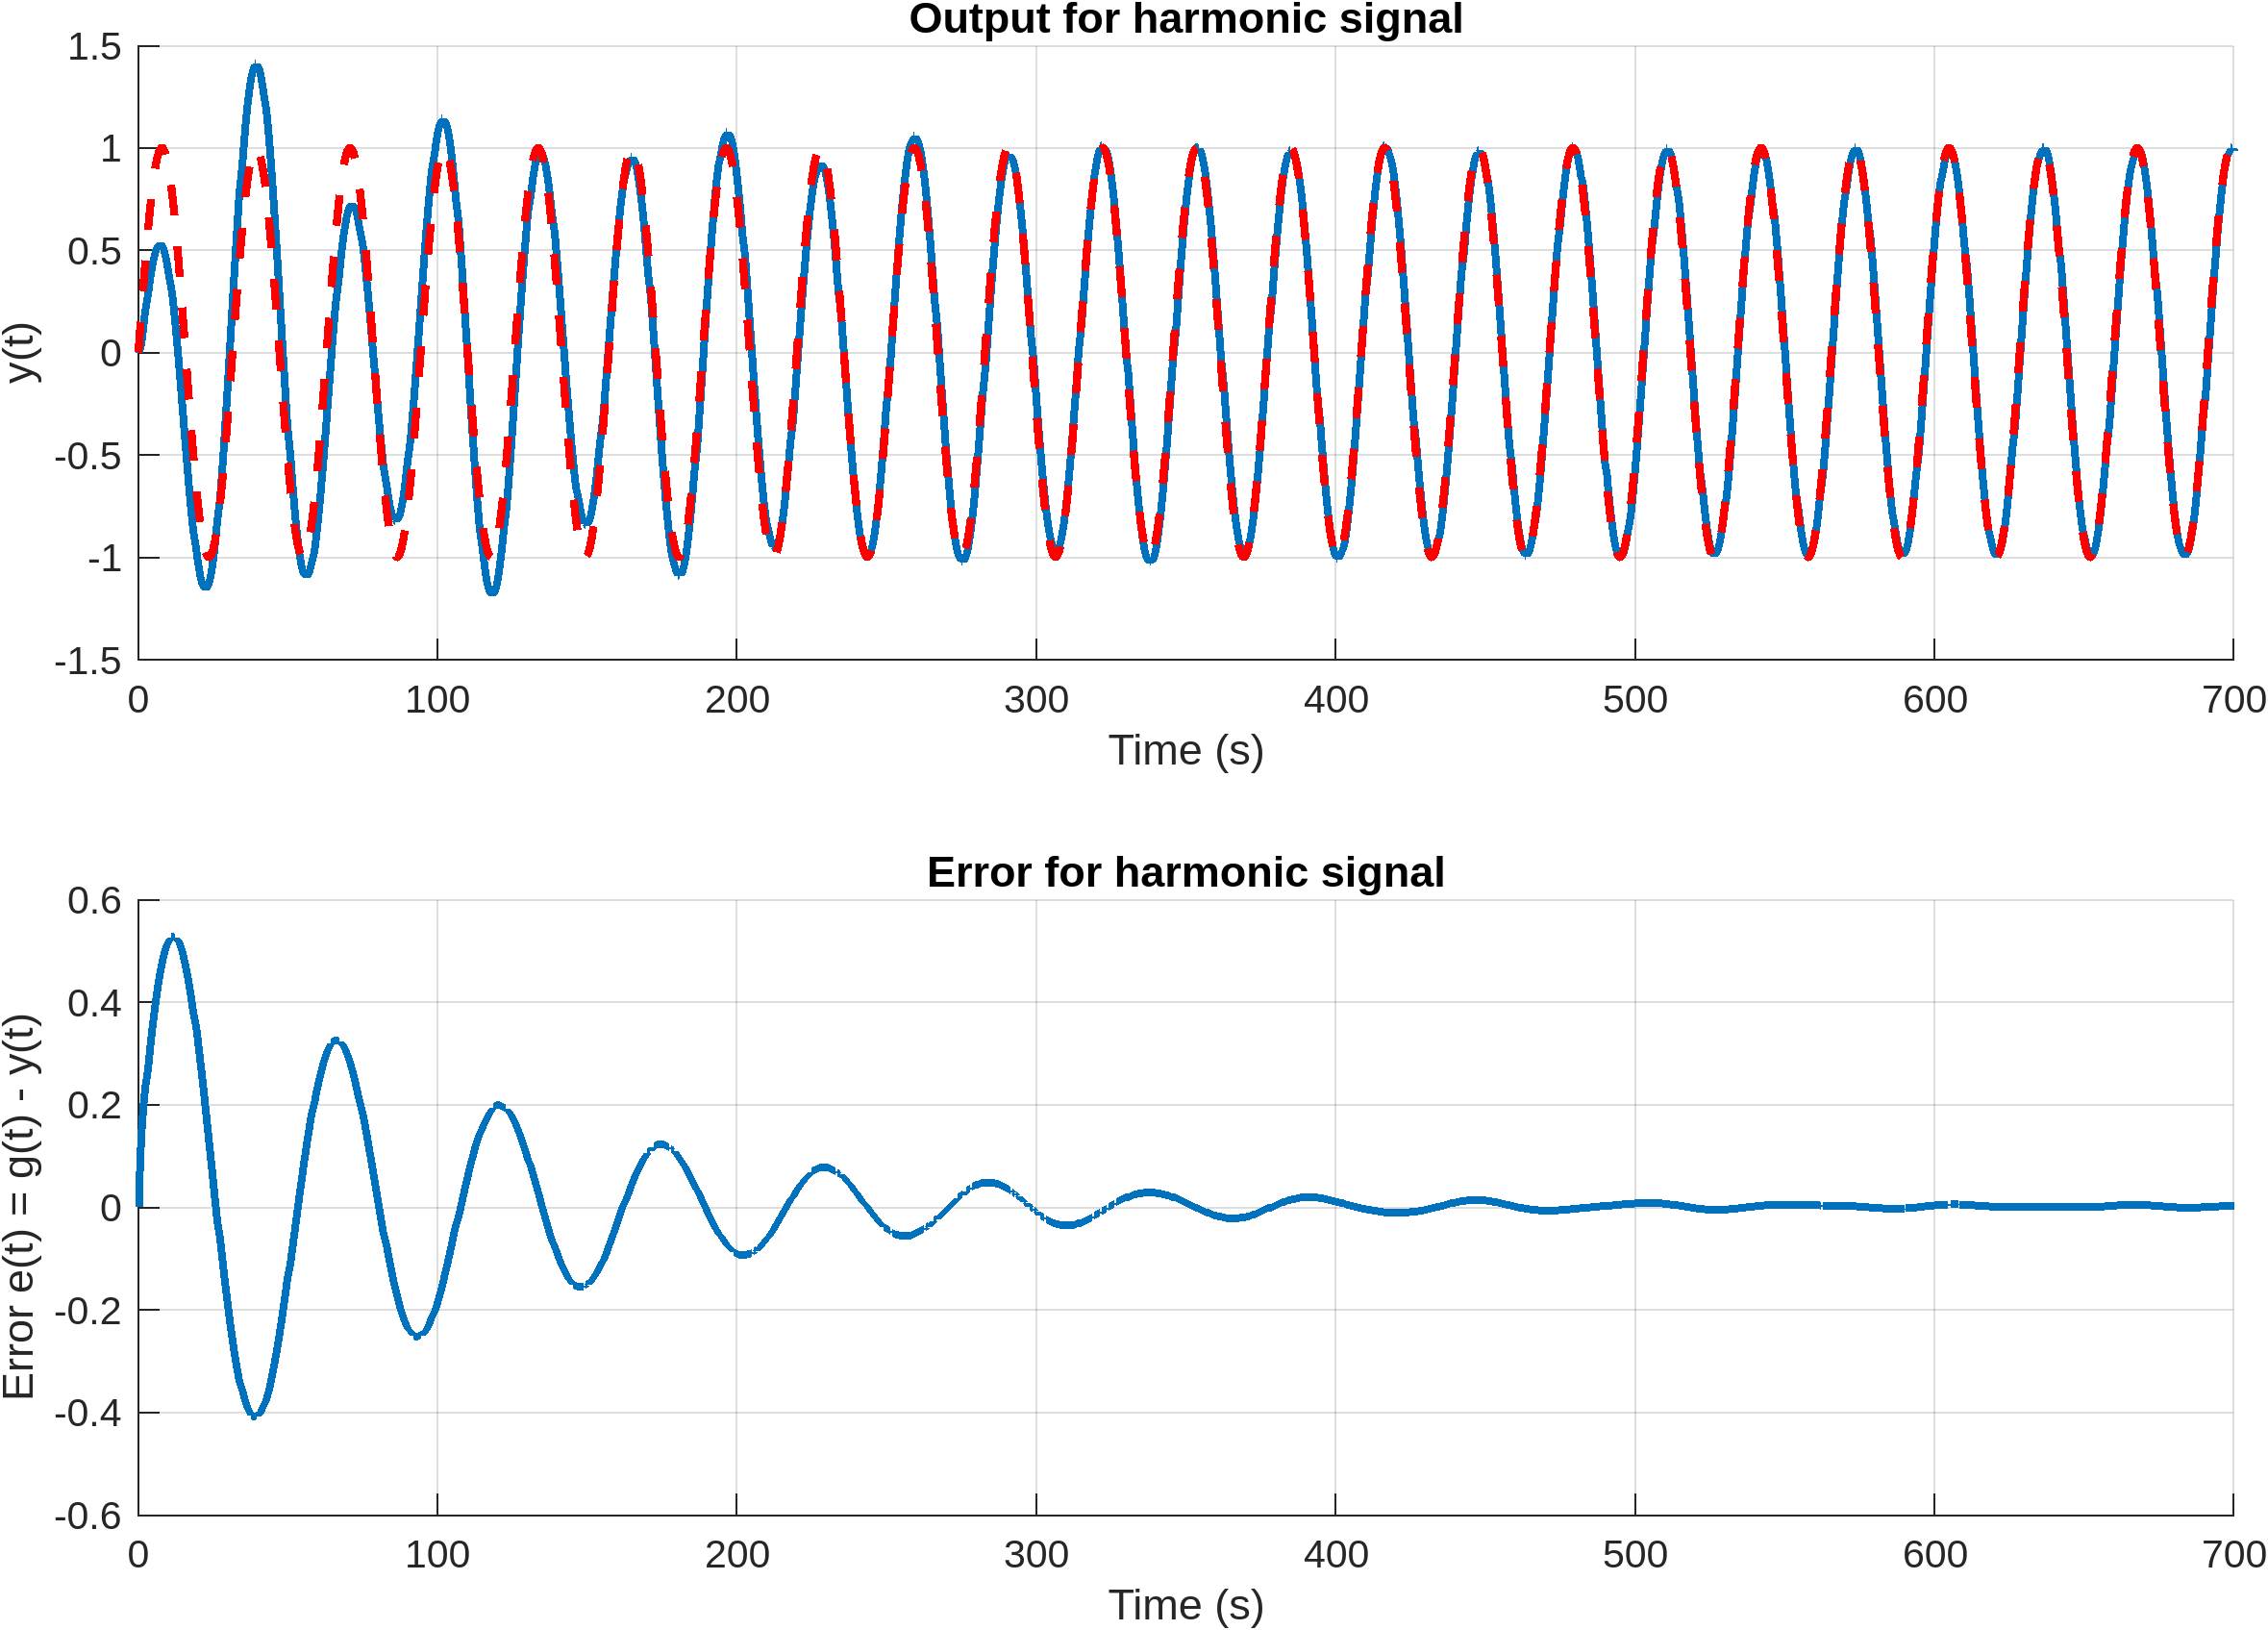
\includegraphics[width=0.8\textwidth]{figs/task_6_out_harmonic.png}
    \caption{Графики выхода и ошибки системы со специальным регулятором в режиме слежения за гармоническим сигналом}
    \label{fig:task_6_out}
\end{figure}



\section{Заключение}

В процессе выполнения лабораторной работы была решена задача стабилизации
неустойчивой системы с ПД регулятором в двух ``формах'': с идеальным дифференцирующим звеном
и с реальным дифференцирующим звеном, в последнем приближалась дифференциальная часть,
так как Д регулятор физически не реализуем. Далее успешно решались задачи слежения 
за константым, с постоянной скоростью, постоянным ускорением и грамоническим сигналами,
с помощью П, И, ПИ и специальным регуляторами. 


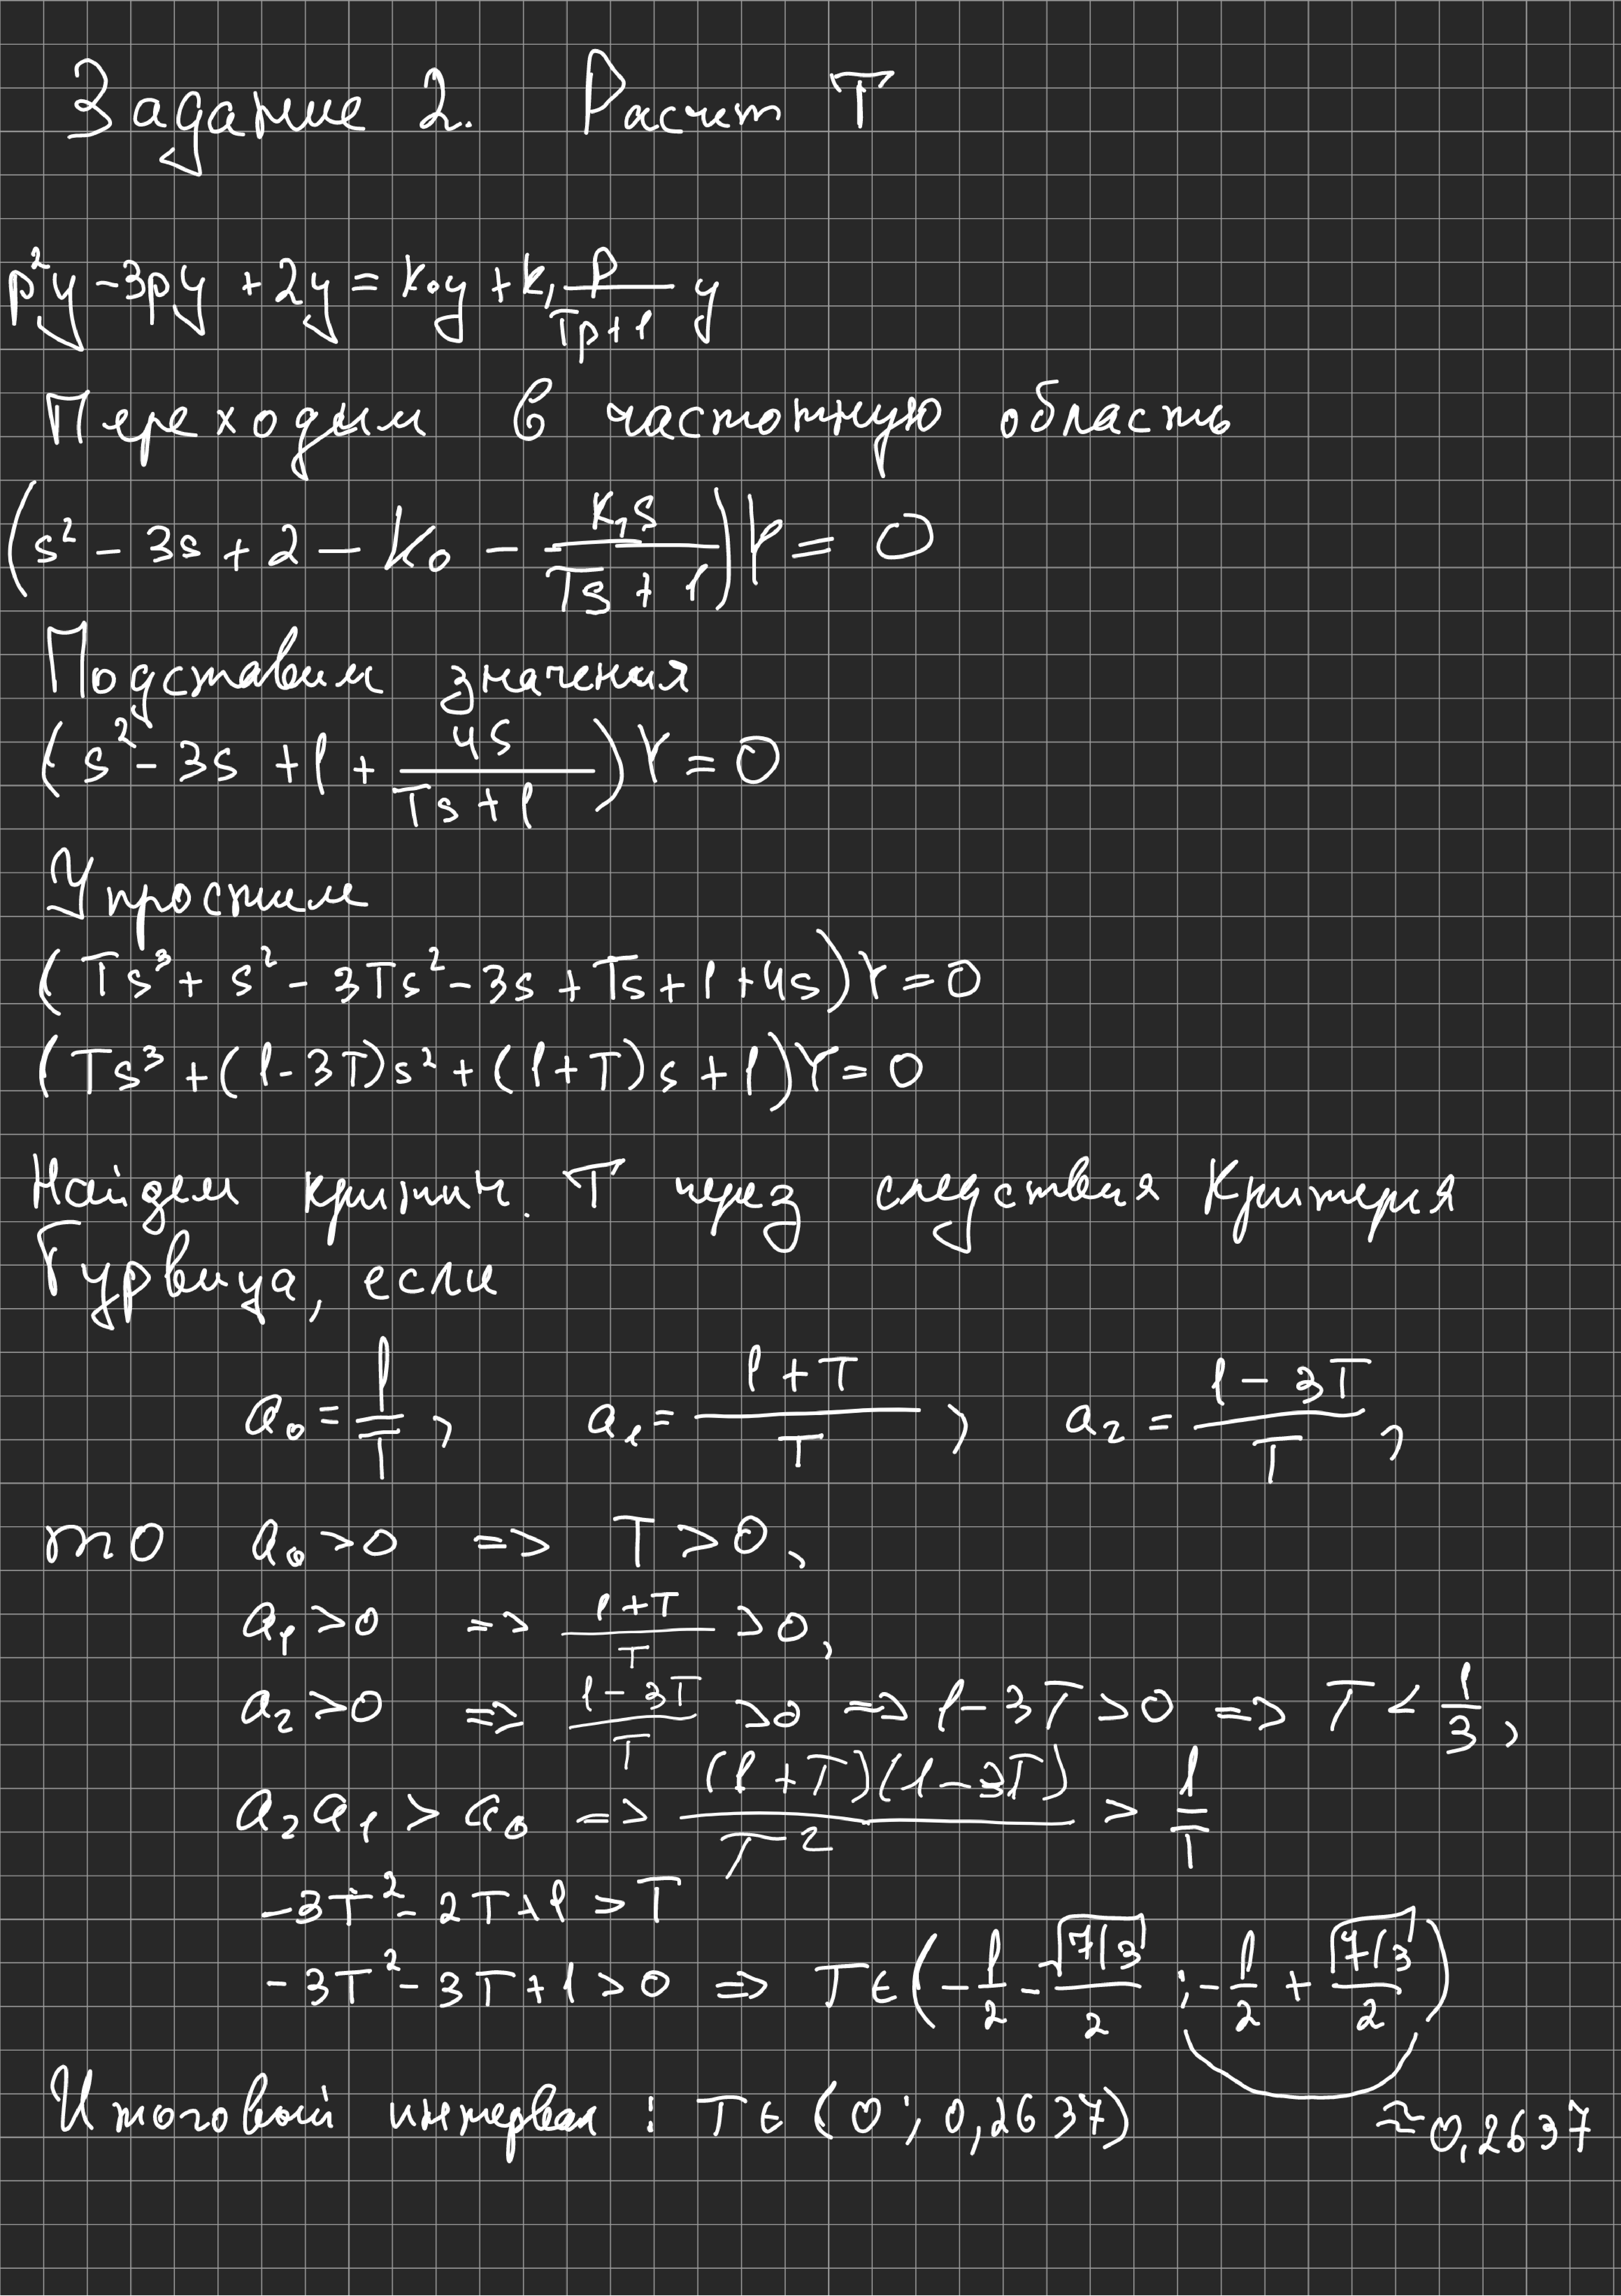
\includepdf[pages=-,scale=1]{figs/task_2_calc.pdf}
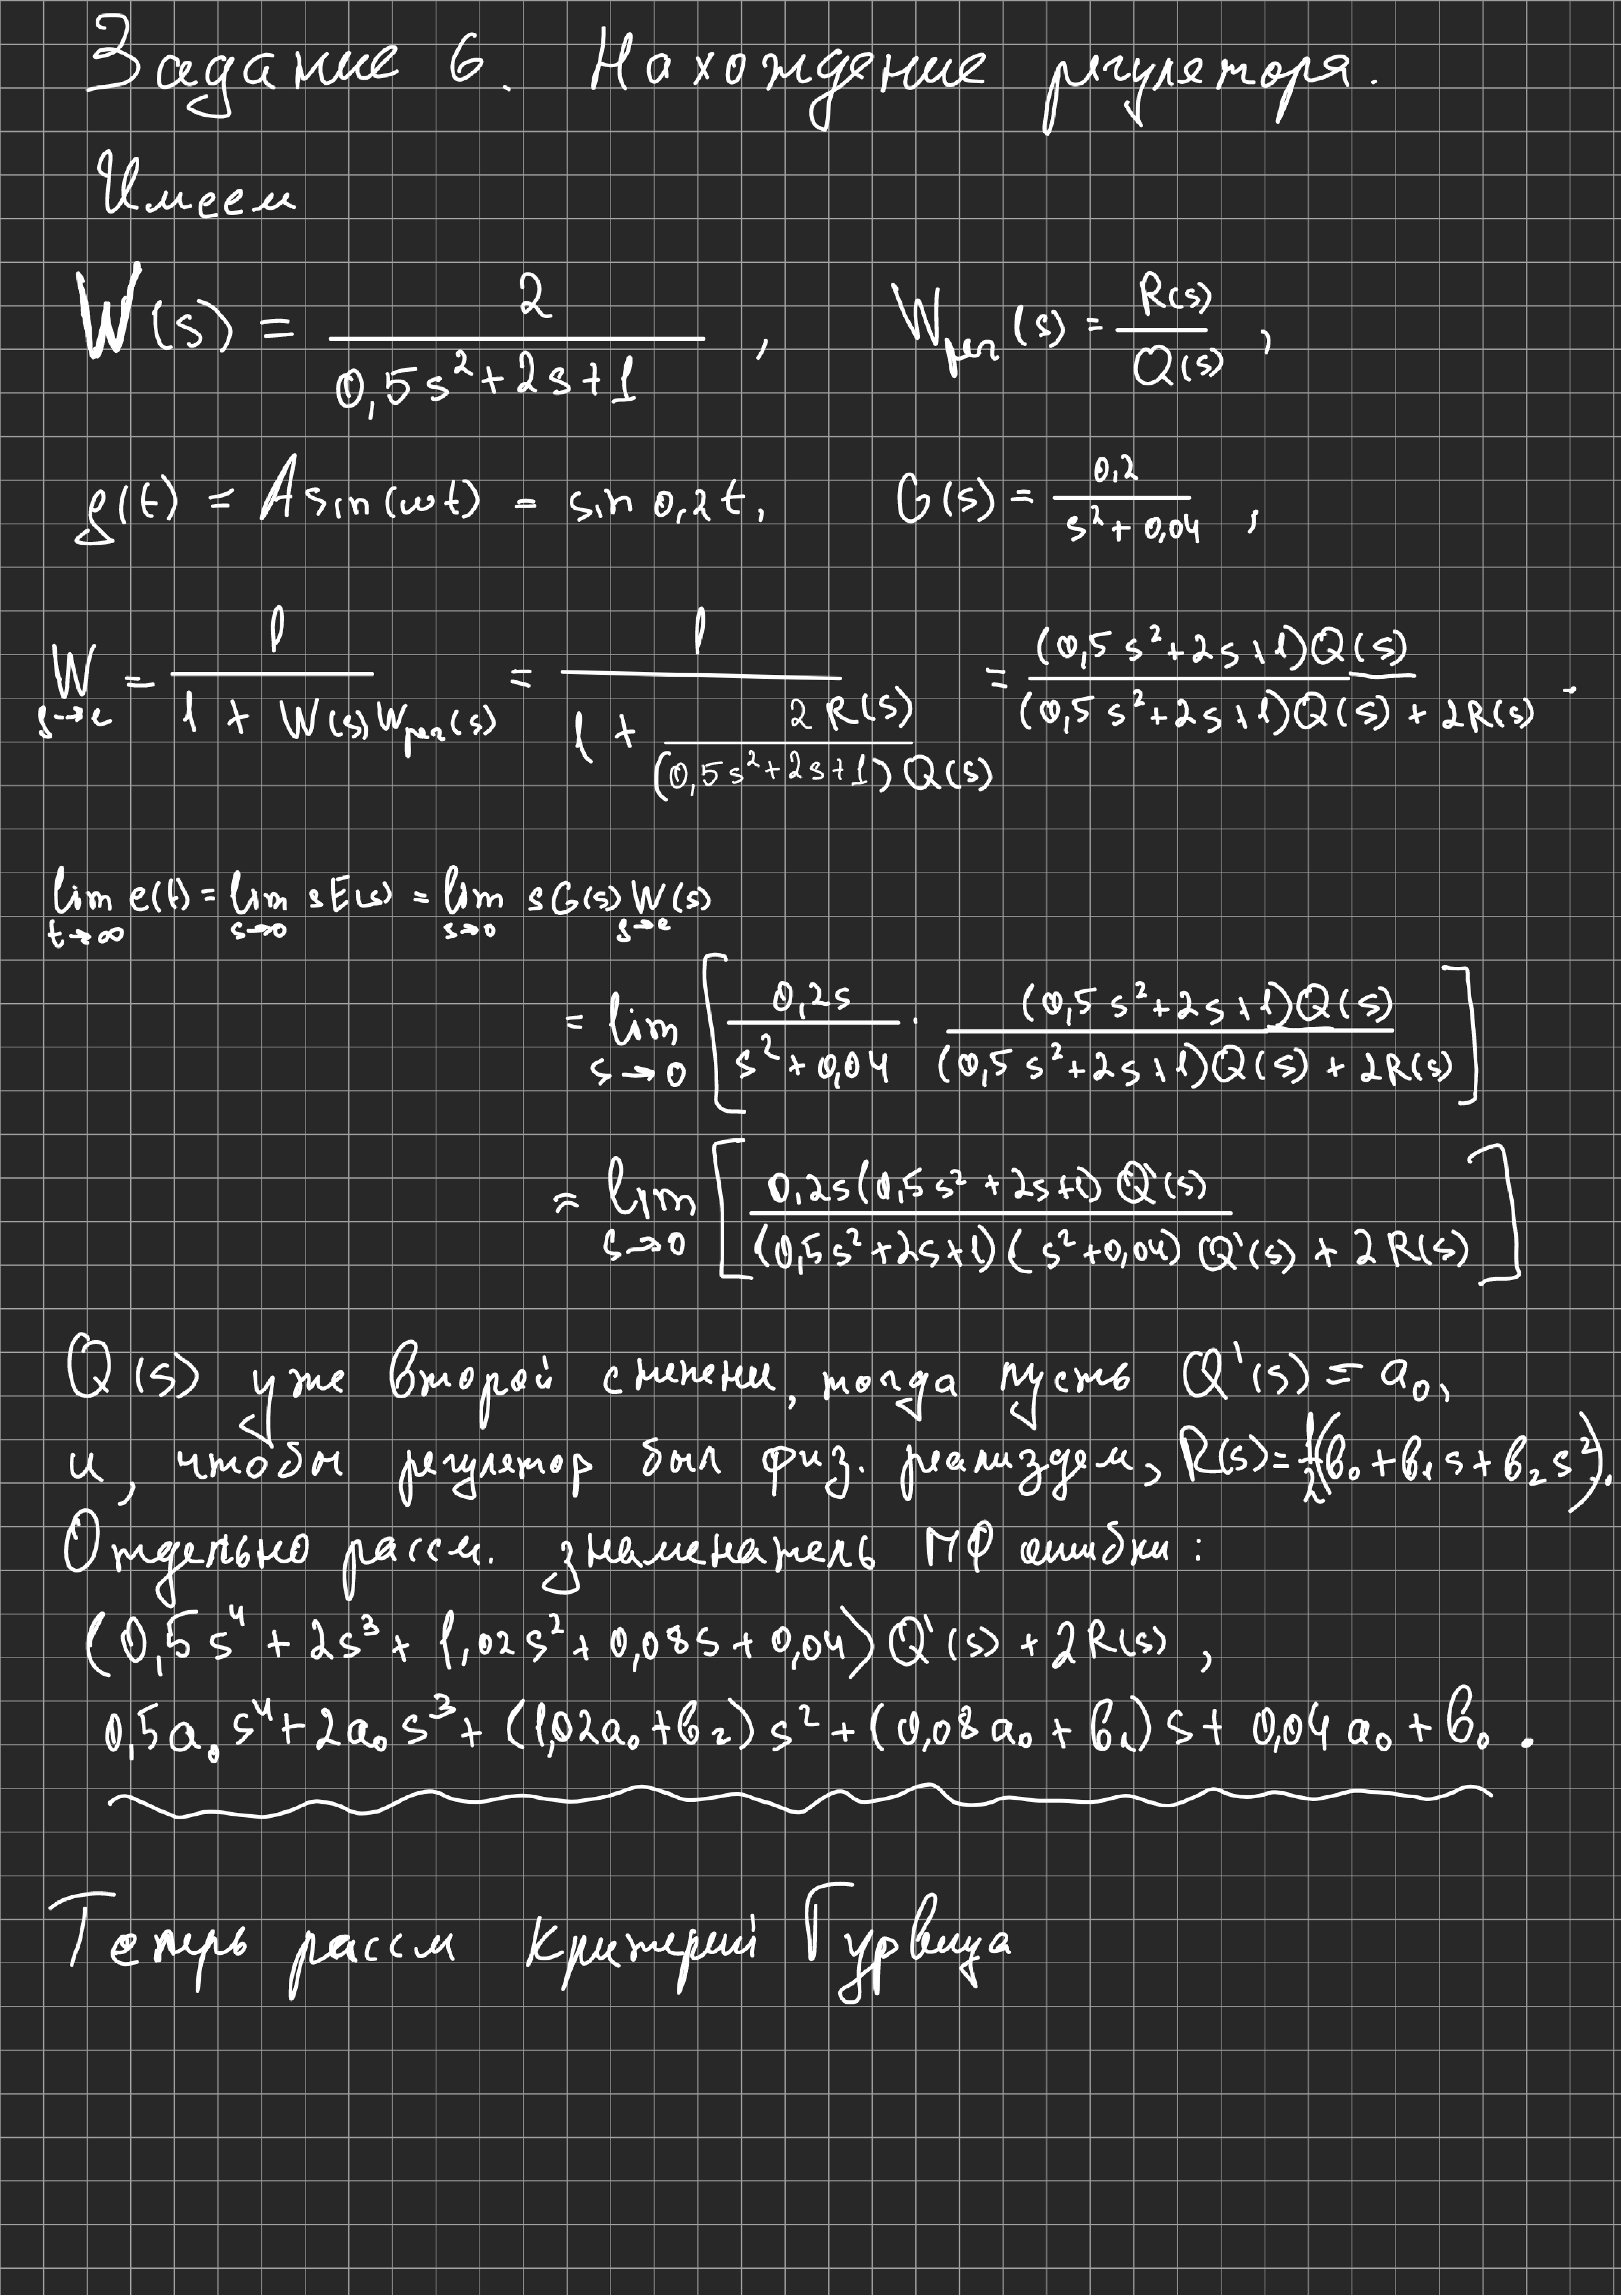
\includepdf[pages=-,scale=1]{figs/task_6_calc.pdf}